%loads the class that provides the titlepage and some general packages.
\documentclass{UniVieCS_Thesis} 

%add the additional packages and macros that you want to use
%here you can find some useful additional packages and macros

%Package to show algorithms
\usepackage{algorithm2e}

%package to work with glossaries
\usepackage[acronym]{glossaries}

%packages and setings to show colored code
\usepackage{listings}
\usepackage{xcolor}

\definecolor{codegreen}{rgb}{0,0.6,0}
\definecolor{codegray}{rgb}{0.5,0.5,0.5}
\definecolor{codepurple}{rgb}{0.58,0,0.82}
\definecolor{backcolour}{rgb}{0.95,0.95,0.92}

\lstdefinestyle{mystyle}{
    backgroundcolor=\color{backcolour},   
    commentstyle=\color{codegreen},
    keywordstyle=\color{magenta},
    numberstyle=\tiny\color{codegray},
    stringstyle=\color{codepurple},
    basicstyle=\ttfamily\footnotesize,
    breakatwhitespace=false,         
    breaklines=true,                 
    captionpos=b,                    
    keepspaces=true,                 
    numbers=left,                    
    numbersep=5pt,                  
    showspaces=false,                
    showstringspaces=false,
    showtabs=false,                  
    tabsize=2
}

\lstset{style=mystyle}

%package to allow comments/notes by you and other people
\usepackage[multiuser,marginclue,nomargin,inline,index]{fixme}
\definecolor{ttwgreen}{RGB}{75,135,73}
\fxusetheme{colorsig}
%\FXRegisterAuthor{tm}{atm}{\color{red}TM}
\FXRegisterAuthor{ttw}{attw}{\color{ttwgreen}TTW} % creates ttwnote, ttwwarning, ttwerror, ttwfatal commands
%\FXRegisterAuthor{mk}{amk}{\color{blue}MK}

%add your own packages or macros here

% important update for glossaries, before document 
\loadglsentries{C) Back Matter/acronyms.tex}
\loadglsentries{C) Back Matter/glossary.tex} 
\makeglossaries %https://www.overleaf.com/learn/latex/glossaries

%shows fixme notes
%\fxsetup{status=draft} % comment/delete this line if you want to your final output

\usepackage[ngerman, british]{babel} %if changed to \usepackage[ngerman]{babel} "Table of contents" changes to "Inhaltsverzeichnis", "abstract" becomes "Zusammenfassung" and "references" is translated to "Literatur".


%remove all the things you don't need and add all the things you need. you can also change the order of the elements at your will.
\begin{document}

    %Start with front matter
    
    %Choose the titlepage you want to use
    
    % --CHANGE THE TITLEPAGE HERE

% title page provided in Word by the University which can be found here 
% https://informatik.univie.ac.at/studium/hilfe-fuer-studierende/wegweiser-masterstudium/approbation-der-masterarbeit/ 
% Please pay attention to the guidelines that can be found there!
%


% There are some commands also for multiple lines. If something exceeds more than a line use the multi line commands. In the worst case adjust the vertical spaces within the class.
% -- Title Page
\Title{Characterizing the Fractal Dimension of Molecular Clouds} 
% A title exceeding one line can be created using the \TitleTwo or \TitleThree command
% \TitleTwo{I wish I \\ had a Master's Degree}
% \TitleThree{I wish I \\ had a Master's \\ Degree}
\Who{Simone Spedicato BSc} %Make sure you add all your titles! 
% A name exceeding one line can be created using the \WhoTwo command
% \WhoTwo{ FirstName \\ LastName BSc}
\Degree{Master of Science (MSc)}
\Year{2025}
\ProgrammeCode{066 861}
\ProgrammeName{Master Astronomy} %Make sure it has the same Name as in the Studienblatt
\Supervisor{Assoz. Prof. Dr. Alvaro Hacar Gonzalez, MA}
% \SupervisorTwo{Second Row} % Here you can change the row under the supervisor
\CoSupervisor{0} %remove this line if there is a Co supervisor
% \CoSupervisor{Professor Co}
% \CoSupervisorTwo{Second Row} % Here you can change the row under the cosupervisor

\Titlepage %This generates the titlepage %Creates the titlepage
    %% --CHANGE THE TITLEPAGE HERE

% title page provided in Word by the University which can be found here 
% https://informatik.univie.ac.at/studium/hilfe-fuer-studierende/bachelorarbeit-empfehlungen/ 
% Please pay attention to the guidelines that can be found there!
% If you want you can always create the titlepage in Word and then add it with \includepdf{<filename>} from the pdfpages package to your thesis.
%


%Do not change or delete the following two lines
\renewcommand{\TitleSetup}{BACHELORARBEIT / BACHELOR'S THESIS}
\renewcommand{\TitleTitleSetup}{Titel der Bachelorarbeit / Title of the Bachelor's Thesis\par}
% Change the rest of the lines to fit you thesis

% There are some commands also for multiple lines. If something exceeds more than a line use the multi line commands. In the worst case adjust the vertical spaces within the class.
% -- Title Page
\Title{I wish I had a Bachelor's Degree} 
% A title exceeding one line can be created using the \TitleTwo or \TitleThree command
%\TitleTwo{I wish I \\ had a Bachelor's Degree}
%\TitleThree{I wish I \\ had a Bachelor's \\ Degree}
\Who{ FirstName LastName } %Make sure you add all your titles! 
% A name exceeding one line can be created using the \WhoTwo command
%\WhoTwo{ FirstName \\ LastName }
\Degree{Bachelor of Science (BSc)}
\Year{2019}
\ProgrammeCode{126489}
\ProgrammeName{Masterstudium Informatik} %Make sure it has the same Name as in the Studienblatt
\Supervisor{Univ. Prof. My favorite professor, PhD}
%\SupervisorTwo{Second Row} % Here you can change the row under the supervisor
\CoSupervisor{0} %remove this line if there is a Co supervisor
\CoSupervisor{Professor Co}
\CoSupervisorTwo{Second Row} % Here you can change the row under the cosupervisor

\Titlepage %This generates the titlepage %Creates the titlepage
    %% --CHANGE THE TITLEPAGE HERE

% title page provided in Word by the University which can be found here 
% https://doktorat.univie.ac.at/doktoratsablauf/abschlussphase/einreichen-und-begutachtung/
% Please pay attention to the guidelines that can be found there!
% If you want you can always create the titlepage in Word and then add it with \includepdf{<filename>} from the pdfpages package to your thesis.
%


%Do not change or delete the following two lines
\renewcommand{\TitleSetup}{DISSERTATION / DOCTORAL THESIS}
\renewcommand{\TitleTitleSetup}{Titel der Disseratation / Title of the Doctoral Thesis\par}
% Change the rest of the lines to fit you thesis


% There are some commands also for multiple lines. If something exceeds more than a line use the multi line commands. In the worst case adjust the vertical spaces within the class.
% -- Title Page
\Title{I wish I had a Doctor's Degree} 
% A title exceeding one line can be created using the \TitleTwo or \TitleThree command
%\TitleTwo{I wish I \\ had a Doctor's Degree}
%\TitleThree{I wish I \\ had a Doctor's \\ Degree}
\Who{ FirstName LastName MSc} %Make sure you add all your titles! 
% A name exceeding one line can be created using the \WhoTwo command
%\WhoTwo{ FirstName \\ LastName MSc}
\Degree{Doctor of Philosophy (PhD)}
%\Degree{Doktorin ODER Doktor der >Zusatz< (Dr. >Abkürzung<)}
%\Degree{Doktorin OR Doktor der >affix< (Dr. >abbr.<)}

\Year{2019}
\ProgrammeCode{A 786 880}
\ProgrammeName{Doctoratsstudium Informatik} %Make sure it has the same Name as in the Studienblatt
\Supervisor{Univ. Prof. My favorite professor, PhD}
%\SupervisorTwo{Second Row} % Here you can change the row under the supervisor
\CoSupervisor{0} %remove this line if there is a Co supervisor
\CoSupervisor{Professor Co}
\CoSupervisorTwo{Second Row} % Here you can change the row under the cosupervisor

\Titlepage %This generates the titlepage %Creates the titlepage
    
    \clearpage
	\frontmatter{}
	\thispagestyle{empty}
\chapter{Acknowledgements}

Thank you! 
\clearpage
%\cleardoublepage{} %adds the aknowledgements
			%Please consider the following section of the "Formvorschriften für die gedruckte Version"
	%Im Anhang ist eine Zusammenfassung (Abstract) mitzubinden. 
	%Ist die Arbeit in einer Fremdsprache verfasst, ist im Anhang jedenfalls eine deutsche Zusammenfassung mitzubinden.
\chapter{Abstract}
		This \LaTeX{} template provides example on how to format and display text, 
		mathematical formulas, and insert tables or images. There is a lot more you 
		can do with \LaTeX{}, for more information check out https://en.wikibooks.org/wiki/LaTeX.
 % adds the abstract
	\chapter{Kurzfassung}

Die Struktur von Molekülwolken ist entscheidend für das Verständnis der physikalischen Prozesse, die die Sternentstehung steuern. In dieser Arbeit präsentieren wir eine detaillierte morphologische und topologische Analyse der Molekülwolken Orion~A und Orion~B mithilfe von Methoden der Fraktalgeometrie und Minkowski-Funktionale. Auf Basis von Säulendichtekarten, die aus Staubemissionen im fernen Infrarot gewonnen wurden, bestimmen wir sowohl globale als auch lokale fraktale Dimensionen über einen breiten Dynamikbereich hinweg.

Unsere Ergebnisse zeigen in Orion~A einen strukturellen Übergang bei einer Säulendichte von $N \sim 1{,}2 \times 10^{22} \,\mathrm{cm}^{-2}$, der mit dem Auftreten dichter Kerne und erhöhter Sternentstehungsaktivität zusammenfällt. Orion~B hingegen weist eine durchgängig skalenfreie, turbulente Morphologie ohne einen solchen Übergang auf. Die Euler-Charakteristik untermauert diese Interpretation durch ein deutliches topologisches Maximum in Orion~A, das in Orion~B fehlt. 

Zusätzlich führen wir eine lokale Karte der fraktalen Dimension sowie sogenannte Masse–Größe–Dimensions–Diagramme (MSD) ein, um die strukturelle Komplexität ortsaufgelöst zu analysieren. Ein Vergleich mit der Verteilung junger Sternobjekte (YSOs) zeigt, dass Regionen mit höherer fraktaler Komplexität insbesondere in Orion~A vermehrt frühe Entwicklungsstadien der Sternentstehung aufweisen. Dies deutet auf eine Verbindung zwischen komplexer Morphologie und aktiver Sternbildung hin.

Unsere Arbeit zeigt, wie Methoden der Fraktal- und Topologieanalyse helfen können, die mehrskalige Struktur des interstellaren Mediums zu erfassen und mit physikalischen Prozessen der Sternentstehung zu verknüpfen.

\clearpage %adds the "Kurzfassung"in german.
	\pagebreak
	
    \microtypesetup{protrusion=false}
    \tableofcontents{}
    % Use an optional list of tables / figures / algorithms / listings(code).
    \listoftables 
    \listoffigures
    \cleardoublepage{}
    % \listofalgorithms
    % \addcontentsline{toc}{chapter}{List of Algorithms} 
    % \cleardoublepage{}
    % \lstlistoflistings
    % \cleardoublepage{}
    \microtypesetup{protrusion=true}
    
	\pagebreak
	
	%add your chapters here
	\mainmatter{}
    \chapter{Introduction}

Giant Molecular Clouds (GMCs) are the primary sites of star formation in galaxies \cite{mckee2007theory}. Within these massive, cold, and dense regions, stars form from the gravitational collapse of the highest column density structures. Understanding the morphology and internal structure of GMCs is therefore essential to understanding the conditions that regulate star formation.

Much of our knowledge of GMC structure comes from the study of dust emission \cite{draine2003interstellar}. Dust grains— well-coupled to the gas in these clouds—emit thermal radiation in the far-infrared and submillimeter regimes. These emissions can be used to reconstruct column density maps, offering a valuable window into the distribution of material within the cloud.

To go beyond qualitative visual interpretation, quantitative tools are needed to describe the spatial complexity of these structures. One powerful approach involves applying methods from fractal geometry and topology. The concept of a fractal dimension, first introduced by Mandelbrot, provides a way to quantify the irregularity or complexity of a structure's boundary \cite{cannon1984fractal}. Complementary topological measures, such as the Minkowski functionals, allow us to describe properties like connectivity and fragmentation.

Historically, various techniques have been employed to estimate the fractal dimension of molecular clouds—from simple box-counting algorithms to power-law scalings of structure size distributions \cite{elmegreen1996fractal}. However, these methods can often provide a limited or averaged view of complex, hierarchical structures.

The motivation behind this thesis is to develop and apply tools that connect the visual complexity of molecular clouds with physically meaningful, measurable quantities. By refining the analysis of fractal and topological properties, we aim to gain deeper insight into the role of turbulence, structure formation, and star formation in GMCs in a new fashion.

The goals of this thesis are:
\begin{itemize}
    \item to extract and preprocess observational column density data for selected GMCs,
    \item to characterize their structure using topological methods such as the Euler characteristic and perimeter–area scaling,
    \item to explore the fractal dimension framework in both global and local forms, and
    \item to investigate correlations between structural complexity and star formation indicators.
\end{itemize}

The thesis is organized as follows:
\begin{itemize}
    \item \textbf{Chapter 2} provides theoretical background on molecular clouds and fractal geometry.
    \item \textbf{Chapter 3} describes the datasets employed, including how column density maps and YSO catalogs are used.
    \item \textbf{Chapter 4} outlines the methods used to calculate fractal and topological descriptors, with a focus on perimeter–area relations and dendrogram-based analysis.
    \item \textbf{Chapter 5} presents the results, including fractal dimension maps, topological behavior, and the relationship between cloud structure and star formation.
    \item \textbf{Chapter 6} discusses the implications of the results and compares them with previous literature and theoretical expectations.
    \item \textbf{Chapter 7} summarizes the main findings and outlines possible directions for future research.
\end{itemize}

Additional material, including simulation details and visual examples of structures, is provided in the Appendices.

    \chapter{Background}
\label{chap:background}

\section{Dust Modeling}

Interstellar dust plays a fundamental role in tracing the structure of molecular clouds (CITATION). Though it accounts for only about 1\% of the mass of the interstellar medium (ISM), its ability to absorb, scatter, and re-emit radiation makes it an essential tool for indirectly probing the properties of cold, dense gas where stars form.

\subsection{Emission from Dust Grains}

Dust grains absorb ultraviolet (UV), visible, and near-infrared (NIR) radiation from stars and re-emit this energy thermally at longer wavelengths, primarily in the mid-infrared (MIR), far-infrared (FIR), and submillimeter (sub-mm) regimes. This process is governed by the radiative transfer equation, which couples extinction (absorption and scattering) and emission across the electromagnetic spectrum (CITATION). In molecular clouds, where visual extinction can exceed $A_V > 10$, emission from dust becomes the dominant observable at long wavelengths.

Dust emission is commonly modeled as a modified black-body, or "grey-body," spectrum:
\[
F_\nu^{\mathrm{obs}} = B_\nu(T_\mathrm{dust}) \times \left(1 - e^{-\tau_\nu}\right),
\]
where $B_\nu(T_\mathrm{dust})$ is the Planck function at the dust temperature $T_\mathrm{dust}$, and $\tau_\nu$ is the optical depth at frequency $\nu$. For optically thin emission at long wavelengths ($\tau_\nu \ll 1$), this simplifies to:
\[
F_\nu^{\mathrm{obs}} \approx B_\nu(T_\mathrm{dust}) \cdot \tau_\nu.
\]

The optical depth $\tau_\nu$ is typically parameterized as:
\[
\tau_\nu = \kappa_\nu \cdot \Sigma,
\]
where $\kappa_\nu$ is the dust opacity and $\Sigma$ the dust surface density. The dust opacity is often modeled as a power-law:
\[
\kappa_\nu \propto \nu^\beta,
\]
where $\beta$ is the dust emissivity index, typically between 1.5 and 2 in the ISM.

\subsection{Rayleigh–Jeans Approximation and FIR Observations}

To reduce the number of free parameters when inferring dust properties, observations are often carried out in the Rayleigh–Jeans (RJ) regime, where $h\nu \ll k_B T$. This condition is typically satisfied at wavelengths longer than $\sim 250\,\mu$m for dust temperatures around $T_\mathrm{dust} \sim 10$–$20$ K, which makes submillimeter and millimeter observations (e.g. from \textit{Herschel}) particularly valuable.

In this regime, the flux scales as:
\[
F_\nu^{\mathrm{obs}} \propto \nu^{2+\beta},
\]
allowing for simplified spectral energy distribution (SED) fitting to extract the dust temperature and column density.

\subsection{Column Density Estimation}

Under the assumption of fixed dust opacity $\kappa_{850}$ and emissivity index $\beta$, one can solve for the dust optical depth at a reference frequency (e.g., $850\,\mu$m):
\[
\tau_{850} = \frac{I_{850}}{B_{850}(T_\mathrm{dust})}.
\]
Given a calibration between optical depth and column density (e.g., from \cite{hildebrand1983determination}), the molecular hydrogen column density $N(\mathrm{H}_2)$ can be in principle estimated as:
\[
N(\mathrm{H}_2) \propto \tau_{850}.
\]

This method allows for the derivation of full-resolution column density maps from multi-band FIR/sub-mm observations, as performed by the \textit{Herschel} Gould Belt Survey, providing a key data product for structural and fractal analyses.

\subsection{Comparison with Extinction Methods}

\begin{figure}[t]
    \centering
    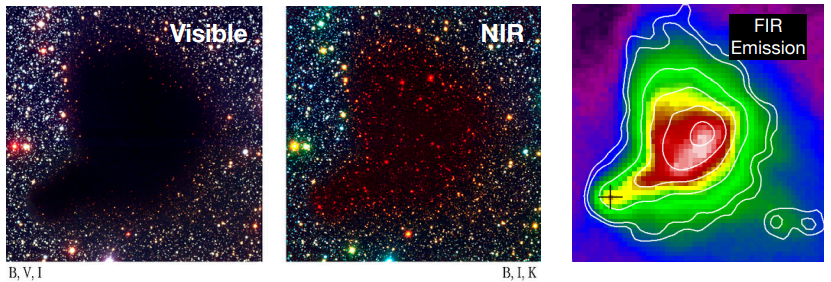
\includegraphics[width=0.75\textwidth]{figures/comparison_dust.png}
    \caption{Comparison of dust extinction (optical and NIR) and dust emission (FIR) views of Barnard 68. Credits: ESO, \cite{nielbock2012earliest}.}
    \label{fig:comparison_dust}
\end{figure}

Dust column densities can also be inferred from extinction measurements, particularly in the near-infrared (e.g., via NICER/NICEST , CITATION). These techniques are independent of dust temperature and often provide high angular resolution in regions with abundant background stars. However, their reliability decreases in high-opacity areas, where few background stars are detectable, and they require robust modeling of the stellar background.

Emission-based methods, by contrast, are more effective in probing dense and cold regions. By modeling the thermal emission from dust at far-infrared and sub-millimeter wavelengths, they can recover column density even where extinction saturates. Nevertheless, these methods rely on assumptions about dust temperature, opacity laws, and emissivity index, which can introduce systematic uncertainties.

Each approach has its strengths and limitations, and the choice between them depends on the scientific objectives and the characteristics of the target region. A visual comparison of both techniques is shown in Figure~\ref{fig:comparison_dust}, highlighting the complementary nature of extinction and emission observations for the dark cloud Barnard 68.

\subsection{Relevance to Star Formation}

Dust-based column density maps are crucial for studying the early stages of star formation. Since most dust in molecular clouds is cold ($T_\mathrm{dust} \sim 10{-}20\,\mathrm{K}$), emission in the FIR/sub-mm naturally traces the dense gas where star formation occurs. Thresholds in column density (e.g., $N(\mathrm{H}_2) \sim 1{-}2 \times 10^{22}\,\mathrm{cm}^{-2}$) have been associated with the onset of core formation and gravitational instability \cite{lada2010star}.

Thus, dust modeling serves as the foundation for the structural and statistical analyses performed throughout this thesis.

\section{Fractals}

Fractals are geometric objects characterized by irregularity and self-similarity over a range of scales. Unlike classical Euclidean shapes, fractals cannot be described by integer dimensions and often exhibit complex, nested structures. Introduced to the scientific community largely through the work of Mandelbrot in the late 20th century (CITATION), fractal geometry has since become a powerful framework for describing naturally occurring structures, from coastlines to clouds.

In the context of molecular clouds, fractal behavior arises seemingly naturally everywhere we look. These regions of the interstellar medium exhibit turbulent dynamics and hierarchical fragmentation, producing morphologies that lack a characteristic scale. Theoretical models of interstellar turbulence, particularly those based on compressible, supersonic flows, predict self-similar density structures (CITATION). Observational studies have consistently found evidence of such fractal-like properties in molecular clouds, supporting the idea that turbulence plays a dominant role in shaping them \cite{elmegreen1996fractal, falgarone1991hierarchical}.

The \emph{fractal dimension} is a key quantitative descriptor of a structure's complexity.  Unlike topological dimension, the fractal dimension can take non-integer values and is sensitive to the method used to estimate it. In this work, we explore this quantity through the perimeter–area relation and other related approaches, which are introduced in detail in later chapters.

Understanding fractal properties is not just a matter of geometry. The morphology of molecular clouds is intimately connected to their physical evolution. For instance, more fragmented structures may reflect advanced stages of gravitational collapse or be the signature of driven turbulence. Moreover, star formation tends to occur in regions of low complexity and high density, suggesting a link between the fractal nature of clouds and their star-forming potential.

In summary, fractal geometry offers an intuitive and quantitative framework to describe the hierarchical, scale-free nature of molecular clouds. Combined with other morphological and topological tools, it provides valuable insights into the processes that govern the interstellar medium and the onset of star formation. Combining these techniques with dust emission maps will allow us to quantitatively characterize the structure of molecular clouds across a wide range of spatial scales. This integrated approach enables the identification of correlations between cloud morphology, physical conditions, and star formation activity, thereby advancing our understanding of the complex interplay between turbulence, gravity, and feedback in the interstellar medium.
    \chapter{Data}
\label{chap:data}

\section{Dust Emission Maps of Orion}
the main data source comes from the ESA's Herschel Space Observatory (generalities on the observatory)

Technicalities of the instruments

Technicalities of the data (dust emission maps) -> Lombardi et al.

In general

Specific to these maps (coverage and such)

Going from dust maps to column density maps...

\section{YSOs}
Extra: YSOs data? TBD


    \chapter{Methods}
\label{ch:methods}

% to-do:
% define global properties and local properties better and clearer!
\section{Introduction}

It is thought that the structure of the interstellar medium (ISM) plays a crucial role in the formation of stars and galaxies. The ISM is a complex and dynamic environment, characterized by a wide range of physical conditions, including temperature, density, and magnetic fields. Understanding the structure of the ISM is essential for understanding how stars and galaxies form and evolve.
Obsevations of the ISM reveal a rich tapestry of structures, ranging from small molecular clouds to large-scale filaments and bubbles. These structures are often characterized by their irregular shapes and complex geometries, which can make them difficult to analyze and interpret.
In this chapter, we will discuss the methods used to analyze the structure of the ISM, with a focus on the Minkowski functionals and the fractal dimension. These methods provide a powerful framework for quantifying the shape and structure of objects in a space, allowing us to derive various properties of the structures, such as their size, shape, and connectivity.

The fractal dimension is a measure of the complexity of the border of a shape, which can calculated using the Minkowski functionals.

\section{Minkowski Functionals}

The Minkowski functionals are a set of topological measures that can be used to quantify the shape and structures of objects in a space. From these functionals, we can derive various properties of the structures, such as their size, shape, and connectivity, but also connect .
These can be defined for any dimension, but we will focus on the 2D case, which is relevant for the analysis of the column density maps.

First it is convenient to define the concept of threshold, which is important both in understanding the methods but also in the application.
Excursion and Level Set: We define the excursion set $S_{\nu}$ of a given field on a $d$-dimensional domain $D \subset R^d$ as the set of points where $f$ exceeds a given threshold parameter $\nu$:

\begin{equation}
    S_{\nu} = \{ \mathbf{x} \in D : f(\mathbf{x}) > \nu \}
\end{equation}

The boundary of the excursion set is defined as the level set, which is the set of points where the field equals the threshold:

\begin{equation}
    \partial S_{\nu} = \{ \mathbf{x} \in D : f(\mathbf{x}) = \nu \}
\end{equation}

An example of these can be seen in Figure \ref{fig:level_set_example}.

\begin{figure}[t]
    \centering
    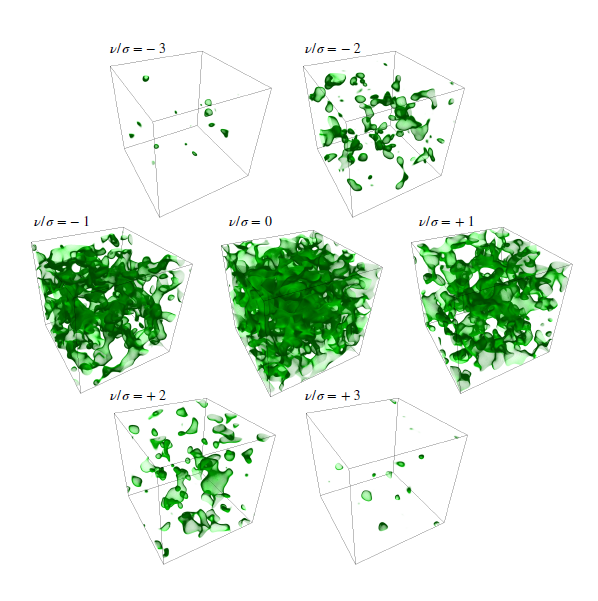
\includegraphics[width=0.6\textwidth]{figures/boundaries.png}
    \caption{Example of an excursion set and its boundary for a field for a smoothed three-dimensional Gaussian field.}
    \label{fig:level_set_example}
\end{figure}

The motion-invariants are defined as the integrals of the Minkowski functionals over the excursion set $S_{\nu}$, are d+1 and are called the Minkowski functionals. For a 2-dimensional map, these are:

\begin{itemize}
    \item $M_0(S_{\nu})$: the area of the excursion set, which is the integral of the field over the set $S_{\nu}$.
    \item $M_1(S_{\nu})$: the perimeter of the excursion set.
    \item $M_2(S_{\nu})$: the Euler characteristic of the excursion set, which is a measure of the connectivity of the set.
\end{itemize}

From these, we can define a lot of properties that can be calculated to characterize the structures in Orion A and B. 

The following section is divided into two parts: global properties and local properties. Global properties are those that describe the overall structure of the ISM, while local properties are those that describe how the structure changes as a function of column density.

\section{Global Properties}

\subsection{Global Fractal Dimension}

The fractal dimension is a measure of the border complexity of a given structure. This can be calculated using the Minkowski functionals, specifically the perimeter and area \cite{cannon1984fractal}. 
The main idea for this approach is that, for a given border length, a simple border will always enclose a larger area than a complex border.

On this idea, the perimeter-area (P-A) relation is defined as:

\begin{equation}
    \label{eq:perimeter_area}
    P = A^{\frac{D}{2}}
\end{equation}

By measuring the perimeter $P$ and area $A$ of a structure at different thresholds and fitting the logarithm of the perimeter to the logarithm of the area, we can derive the fractal dimension $D$ of the overall structure.

The relation between perimeter and area provides information about the complexity or degree of contortion of the boundary. For example, a fixed length of smooth, rounded perimeter can enclose a larger area than a highly irregular or convoluted perimeter. This degree of complexity can be characterized by the dimension $D$ of the perimeter. For smooth shapes, such as circles and squares, the scaling follows $P \propto A^{1/2}$, and thus $D=1$, corresponding to the dimension of a line. As the perimeter becomes increasingly contorted and tends to fold back on itself, effectively filling the plane, the scaling approaches $P \propto A$, and $D$ approaches a value of 2.

If the cloud exhibits structures with a well-defined length scale, we can consider the perimeter to be composed of large-scale features superimposed with small-scale noise or perturbations. In this case, the large- and small-scale structures would show different perimeter–area relations, and consequently, different values of $D$. Therefore, if the perimeter–area relation is characterized by multiple values of $D$ across scales, this would point to the existence of processes operating at characteristic spatial scales, and it would motivate a meaningful distinction between large- and small-scale structure. Conversely, if the perimeter–area relation is consistently described by a single power-law scaling, this indicates the absence of characteristic length scales in the cloud morphology.

Hence, if the linear fit in log–log space is robust, one can argue that the structure lacks a preferred scale and therefore behaves as a fractal. An example of this is illustrated in Figure~\ref{fig:perimeter_area_example}, where data from meteorological clouds were used to derive the fractal dimension of the structures. The slope of the linear fit yields the fractal dimension $D$, providing a quantitative measure of the structural complexity. The lack of a characteristic scale, evidenced by the good fit, suggests that turbulent processes are likely responsible for shaping the observed structures.

\begin{figure}[t]
    \centering
    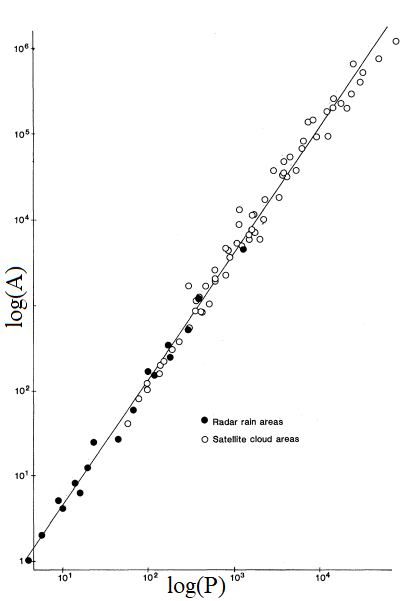
\includegraphics[width=0.45\textwidth]{figures/lovejoy.png}
    \caption{Example of the perimeter-area relation for meteorological clouds \cite{lovejoy1982area}. The slope of the linear fit gives the fractal dimension of the structure.}
    \label{fig:perimeter_area_example}
\end{figure}

This counts in this work a global property of the cloud.

The perimeter-area relation is a powerful tool for analyzing the complexity of structures in the ISM. It's simple, yet effective, and can be applied to a wide range of structures, from clouds to galaxies. The fractal dimension derived from the perimeter-area relation can provide insights into the physical processes that shape these structures, such as turbulence, gravity, and magnetic fields. It is also powerful to analyze the evolution of structures as a function of column density threshold.
However, it is important to note that the perimeter-area relation is not always applicable to all structures. Furthermore, numerical effects can also play a role in the calculation of the fractal dimension, as we will see in the simulations section. Artifacts also have an effect on this method \cite{imre2006artificial}. This is to say, that the method has its limitations and simulations play an important role in understanding these effects. 

\section{Local Properties}

\subsection{Local Fractal Dimension}

One further advantage of the perimeter–area relation is that it can be inverted to derive the fractal dimension of a structure at a given column density threshold. By inverting Eq.~\ref{eq:perimeter_area}, we can express the local fractal dimension $D$ as a function of the column density threshold $\nu$:

\begin{equation}
    \label{eq:local_fractal_dimension}
    D(\nu) = 2 \times \frac{\log\bigl(P(\nu)\bigr)}{\log\bigl(A(\nu)\bigr)}.
\end{equation}

This approach enables a more detailed characterization of the geometry and scaling behavior of the cloud structures as a function of physical conditions. In particular, by applying a series of increasing thresholds $\nu$, one effectively isolates progressively denser substructures within the molecular cloud. At each threshold, the perimeter $P(\nu)$ and area $A(\nu)$ can be measured either for all connected structures collectively or for each identified region individually.

In the first case, the perimeters and areas of all structures present in the map at a given threshold are summed, providing a global measurement of the local fractal dimension for that threshold. This yields a single $D(\nu)$ value for each column density level, capturing how the overall morphological complexity evolves as successively denser material is selected. An example of this approach is shown in Figure~\ref{fig:local_fractal_dimension_example}, where the perimeters and areas are computed across a range of thresholds, demonstrating the dependence of the fractal dimension on the chosen column density cut.

\begin{figure}[t]
    \centering
    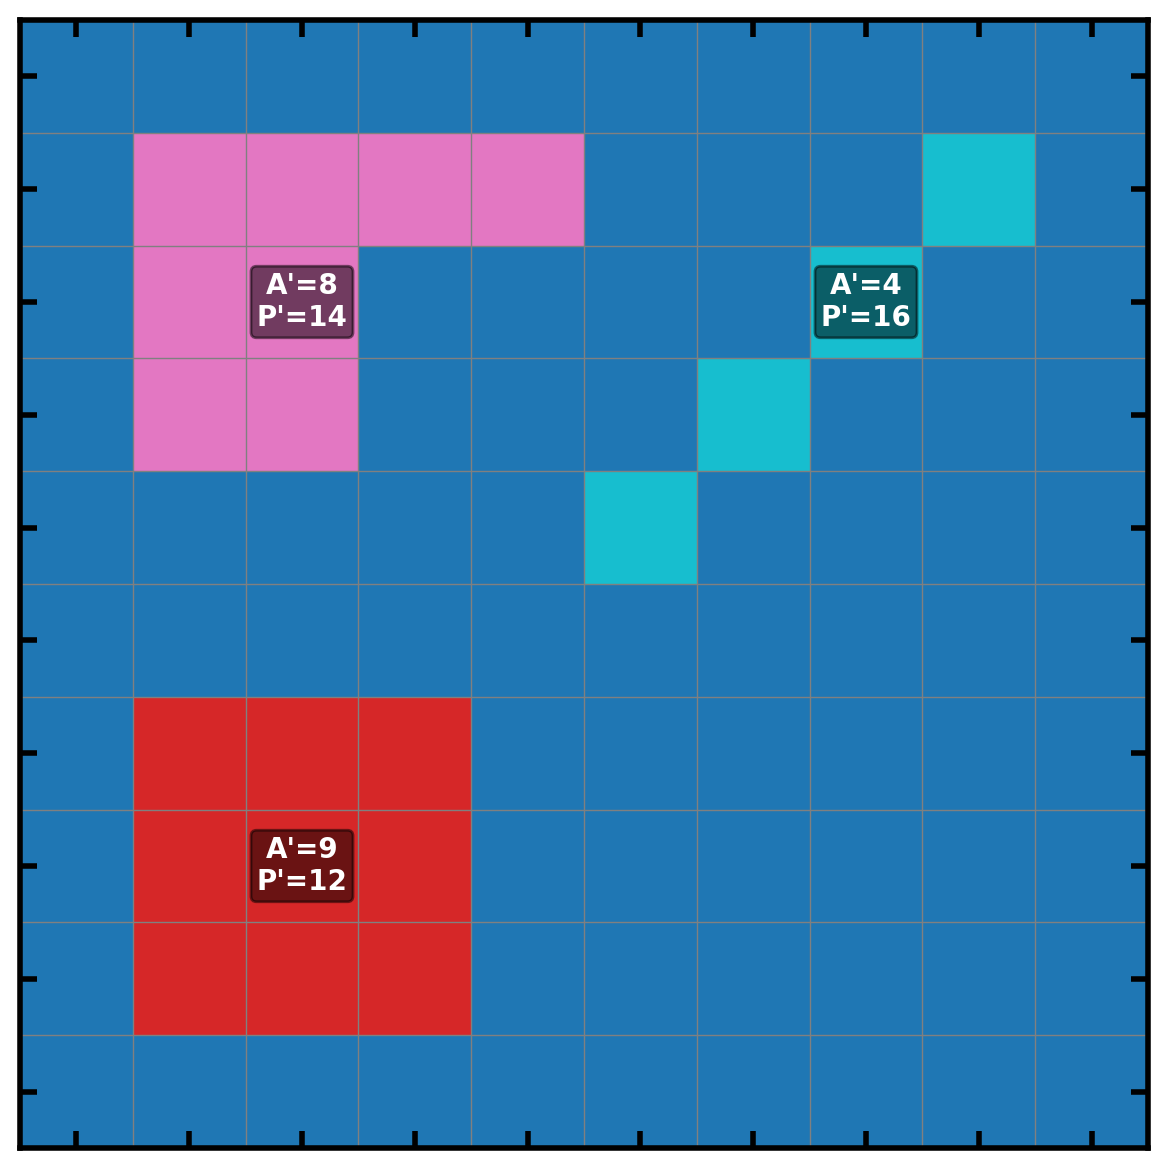
\includegraphics[width=0.5\textwidth]{figures/example_calculations.png}
    \caption{Simplified example of the calculation of perimeters and areas of structures at a given column density threshold. The local fractal dimension can be calculated by summing over all of the structures at that threshold, or for each of the single structures.}
    \label{fig:local_fractal_dimension_example}
\end{figure}

Conversely, it is also possible to calculate the local fractal dimension separately for each individual structure as a function of threshold. In this case, the evolution of $D$ with increasing density can be tracked on a per-object basis, providing insights into whether substructures become more or less fragmented and irregular as higher-density material is isolated. This allows the study of whether certain regions of the cloud exhibit self-similar scaling over a wide range of column densities, or whether there are transitions in the structural properties that may reflect different physical regimes, such as turbulence, gravitational collapse, or feedback from star formation.

Analyzing the local fractal dimension as a function of threshold thus provides a powerful tool to investigate the scale dependence and complexity of molecular clouds, complementing the global measurements and helping to disentangle the contributions from different physical processes.

% to-do: a picture here would not be bad
\subsection{Dendrograms}

In order to explore the segmentation of structures with changing column density or mass, dendrograms are a useful tool. A dendrogram is a diagram that represents the hierarchical organization of structures within the data \cite{everitt2010cambridge}. Specifically, it shows how large-scale regions can be decomposed into smaller substructures as the threshold for the column density (or mass) increases.

By progressively applying higher thresholds, one can trace how individual dense clumps emerge from the diffuse background and how these clumps further fragment into even denser cores. In this way, dendrograms provide a visual and quantitative framework to analyze the nested, multiscale nature of molecular cloud structure.

In this work, dendrograms were constructed using hierarchical clustering methods applied to the mass maps of Orion A and B. This approach allows identification and characterization of the main branches (large coherent structures) as well as the terminal leaves (smallest resolved substructures). For each identified region, properties such as total mass, size (computed via principal component analysis), and fractal dimension were derived to quantify their physical characteristics and complexity.

% to-do: maybe add Alvaro's plot (or maybe in the discussion)
\subsection{Mass-Size-Fractal Dimension (MSD) plane}

Since it is possible to calculate the local fractal dimension for single structure, we can connect this property to more physical aspects of the substructures, namely mass and size. This then allows us to include new information on mass-size diagrams, creating a Mass-Size-Fractal Dimension (MSD).

The dendrogram-like segmentation is an important aspect of this process, as it ensures a proper characterization and recognition of the sub-structures. 

\subsection{Euler characteristic}

Euler characteristic, often denoted as $\chi$ (or $M_2(S_{\nu})$ in the context of the Minkowski functionals), and in two dimensions it is given by:
\begin{equation}
    \chi = \text{Number of connected regions} - \text{Number of holes}
\end{equation}
For a given excursion set $S_{\nu}$, the Euler characteristic provides a measure of the topology of the structures, indicating how many isolated regions and holes are present at a specific threshold. In practice, a positive Euler characteristic indicates more isolated regions than holes, while a negative value suggests a topology dominated by holes.

The Euler characteristic is closely related to the genus $G$ of the structure, where in two dimensions $G = 1 - \chi$. The genus is commonly used in cosmology and astrophysics to describe the connectivity of structures, such as the filamentary network in the ISM or the cosmic web. By analyzing the Euler characteristic or genus as a function of the threshold, one can gain insights into the morphological transitions and connectivity of the observed structures.

\section{Connection to Star Formation}

To investigate the link between cloud structure and star formation activity, we employed the catalogue of young stellar objects (YSOs) compiled by \cite{megeath2012catalogue}.  
This catalogue provides both positional information and evolutionary classifications of YSOs within Orion~A and Orion~B, allowing a direct spatial comparison with the structures identified in our analysis.

The degree of association between the local structural properties and the YSO distribution was quantified using the Pearson correlation coefficient \cite{pearson1895vii} and the Spearman rank correlation coefficient \cite{sedgwick2014spearman}.  
These metrics capture linear and monotonic relationships, respectively, and together provide a robust measure of how variations in the structural parameters relate to the spatial density of YSOs.

We restricted the YSO sample to objects classified as Class I or flat-spectrum sources, based on their infrared slope (\texttt{alpha}) and the catalogue classification flag (\texttt{Cl}). These stages are closely associated with active star-forming regions, while more evolved Class II/III sources may have migrated from their birth sites and were therefore excluded \cite{lada1987star}. For comparison, we also computed correlations using the full YSO sample.

\section{Simulations}

% more details
\subsection{Simulations for the Global Properties}

The simulations addressing the global properties are primarily designed to verify the interpretation of the values obtained for the global fractal dimension $D$, as described in the preceding sections. In particular, they aim to confirm the expectation that the perimeter–area relation should yield unreliable or systematically biased results for structures that possess a well-defined characteristic length scale. 

In this context, Gaussian Random Fields (GRFs) play an important role as a benchmark for comparison. GRFs allow the generation of synthetic structures with controlled statistical properties and scaling behavior, providing a framework to test whether the methodology is sensitive to the presence or absence of intrinsic scales.

\subsection{Simulations for the Local Properties}

Analogously, simulations are employed to better understand how different values of the local fractal dimension arise in different types of structures. These tests include the analysis of Gaussian Random Fields, purely Gaussian noise, and simple geometric shapes such as lines and circles. 

The simulations also allow for quantifying numerical effects and resolution-dependent biases, assessing how limited spatial resolution and discretization influence the measured properties of the identified structures. This helps ensure that the interpretation of the fractal dimension is robust and not merely an artifact of the analysis method or data sampling.

\subsection{Comparison with Other Methods}

In the context of the simulations, a brief comparison with alternative approaches was carried out. This served both to improve understanding of the fractal dimension framework and to identify potential limitations or artifacts of the perimeter–area (PA) method.

The method most frequently used for comparison was the box-counting technique, which relies on covering the shape with a grid of boxes of varying sizes and counting the number of boxes that contain part of the shape. By examining how this count scales with the box size, the fractal dimension can be estimated \cite{falconer2013fractal}. 

\section{Uncertainties}

% Probs need to describe how to go from sigma_P and sigma_A to sigma_D ...
\subsection{Perimeter and Area}

The measurement of perimeter and area is subject to inherent uncertainties. To estimate these uncertainties, the following procedure was carried out:

\begin{itemize}
    \item The perimeter ($P$) and area ($A$) were measured for a set of circles with known true perimeter and area.
    \item The magnitude of the measurement error was computed by comparing the measured values to the true values.
    \item The errors were averaged over a sufficiently large number of samples ($N$) to obtain representative estimates of the typical deviation.
\end{itemize}

\subsection{Beam Size}

The finite resolution imposed by the telescope beam introduces systematic uncertainties in the measurement of structural properties. The beam convolution smooths small-scale fluctuations and reduces the complexity of the contour at each column density threshold. This effect generally leads to an underestimation of the perimeter and an overestimation of the area, biasing the derived fractal dimension toward lower values.

To quantify this uncertainty, one can simulate synthetic column density maps with known fractal characteristics and convolve them with a Gaussian kernel matching the observational beam. By comparing the perimeter–area relations before and after convolution, the bias introduced by the finite resolution can be estimated. Alternatively, the characteristic beam size provides a natural lower limit to the spatial scales where fractal analysis is reliable. In this work, scales smaller than 2–3 times the beam full-width at half-maximum (FWHM) are treated with caution, and the derived fractal dimensions are interpreted as lower limits to the intrinsic complexity of the cloud morphology.

\subsection{Uncertainties in the Extinction Map}

The dataset also includes a pixel-wise $\tau_{850}$ error map, as shown in Figure \ref{fig:error_map}. 

\begin{figure}[t]
    \centering
    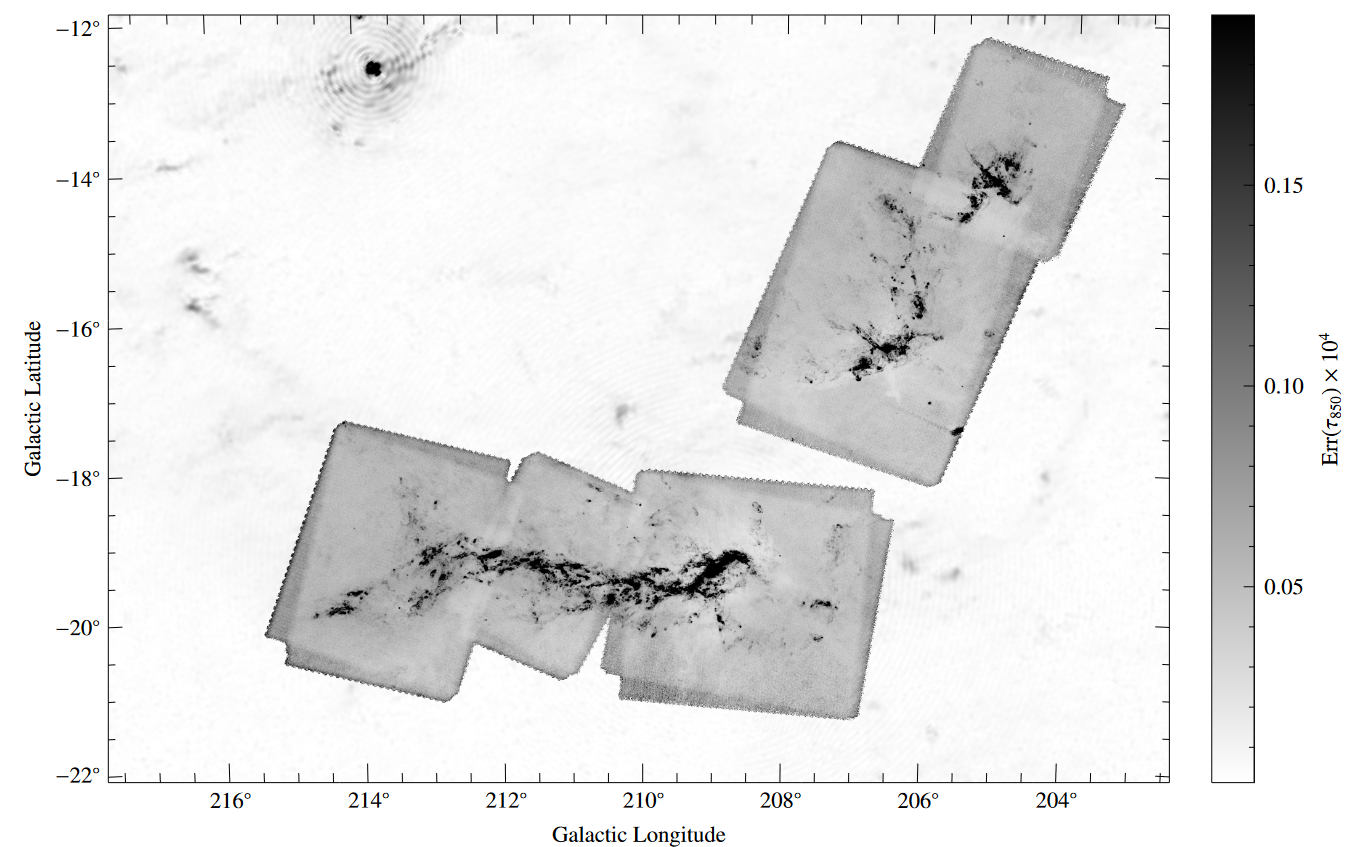
\includegraphics[width=0.6\textwidth]{figures/error_map.png}
    \caption{Pixel-wise error map of the $\tau_{850}$ data \cite{lombardi2014herschel}}
    \label{fig:error_map}
\end{figure}

Although these uncertainties are of a non-negligble magnitude to other sources of error and, in principle, all effects should be taken into account, the dominant contributions to the total uncertainty arise from the measurements of perimeter and area. 
For this reason, the pixel-wise extinction errors are neglected in the following analysis.

    \chapter{Results}
\label{ch:results}

\section{Global Properties}

\subsection{Global Fractal Dimension}

To quantify the cloud morphology through the global fractal dimension, we computed perimeter-area measurements over a restricted range of column densities, \(N_\mathrm{min} \leq N \leq N_\mathrm{max}\), with \(N_\mathrm{min}\) around \(2 \times 10^{21}\,\mathrm{cm}^{-2}\) and \(N_\mathrm{max}\) around \(8 \times 10^{22}\,\mathrm{cm}^{-2}\). This range was chosen to avoid biases caused by the limited angular resolution, which produces artificially smooth contours at low column densities, and by the sparse, irregular features that dominate at the highest column densities. At the same time, this range includes important physical thresholds, such as typical star forming scales and HI to $H_2$ transition regime.

Figure \ref{fig:orion_A_global} shows the perimeter-area relation for Orion A, together with the best-fit linear regression in log-log space used to derive the global fractal dimension. The residuals of the fit are displayed in the lower panel. From this single-fit model we obtain:
\[
D_{\mathrm{OA,\,Global}} = 1.35 \pm 0.02 ,
\]
with a mean absolute residual of 0.1174 and a correlation coefficient of 0.9893.

\begin{figure}[t]
    \centering
    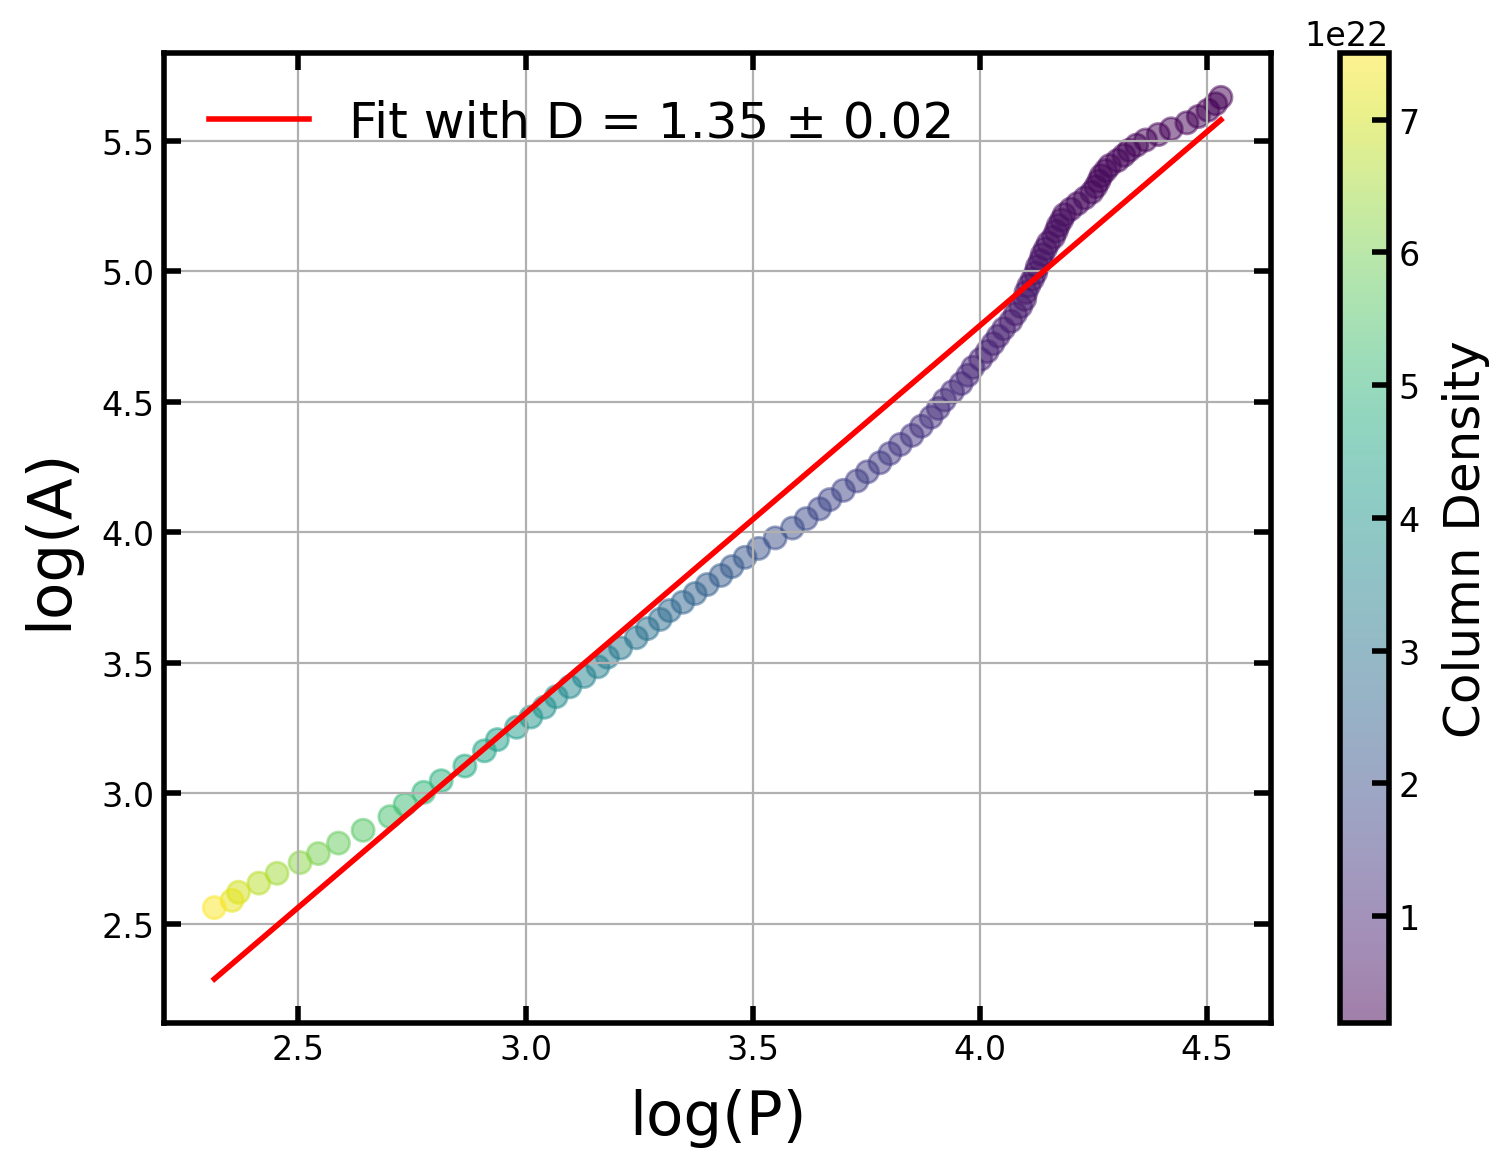
\includegraphics[width=0.5\textwidth]{figures/orion_A_global.png}
    \caption{Perimeter-area relation for Orion A. The solid line indicates the best-fit linear regression in log-log space used to estimate the global fractal dimension \(D_{\mathrm{Global}}\). Residuals are shown in the lower panel.}
    \label{fig:orion_A_global}
\end{figure}

However, the Orion A data show systematic deviations from a single power law across the full column-density range. To account for this, we performed a segmented i.e. double linear fit, dividing the data at \(N = 1.23 \times 10^{22}\,\mathrm{cm}^{-2}\). The two resulting global fractal dimensions from the slopes are:
\[
D_{\mathrm{OA,\,1}} = 1.65 \pm 0.01 \quad \text{(high column density)},
\]
\[
D_{\mathrm{OA,\,2}} = 0.97 \pm 0.3 \quad \text{(low column density)}.
\]
The corresponding mean absolute residuals are 0.0222 (correlation coefficient = 0.9986) for the high-density regime and 0.0679 (correlation coefficient = 0.9748) for the low-density regime, representing a clear improvement compared to the single-fit model.  
Figure \ref{fig:orion_A_global_double_fit} shows the two fitted segments and their residuals. The distinct change in slope suggests a structural transition or the coexistence of different regimes of spatial complexity in Orion A.

\begin{figure}[t]
    \centering
    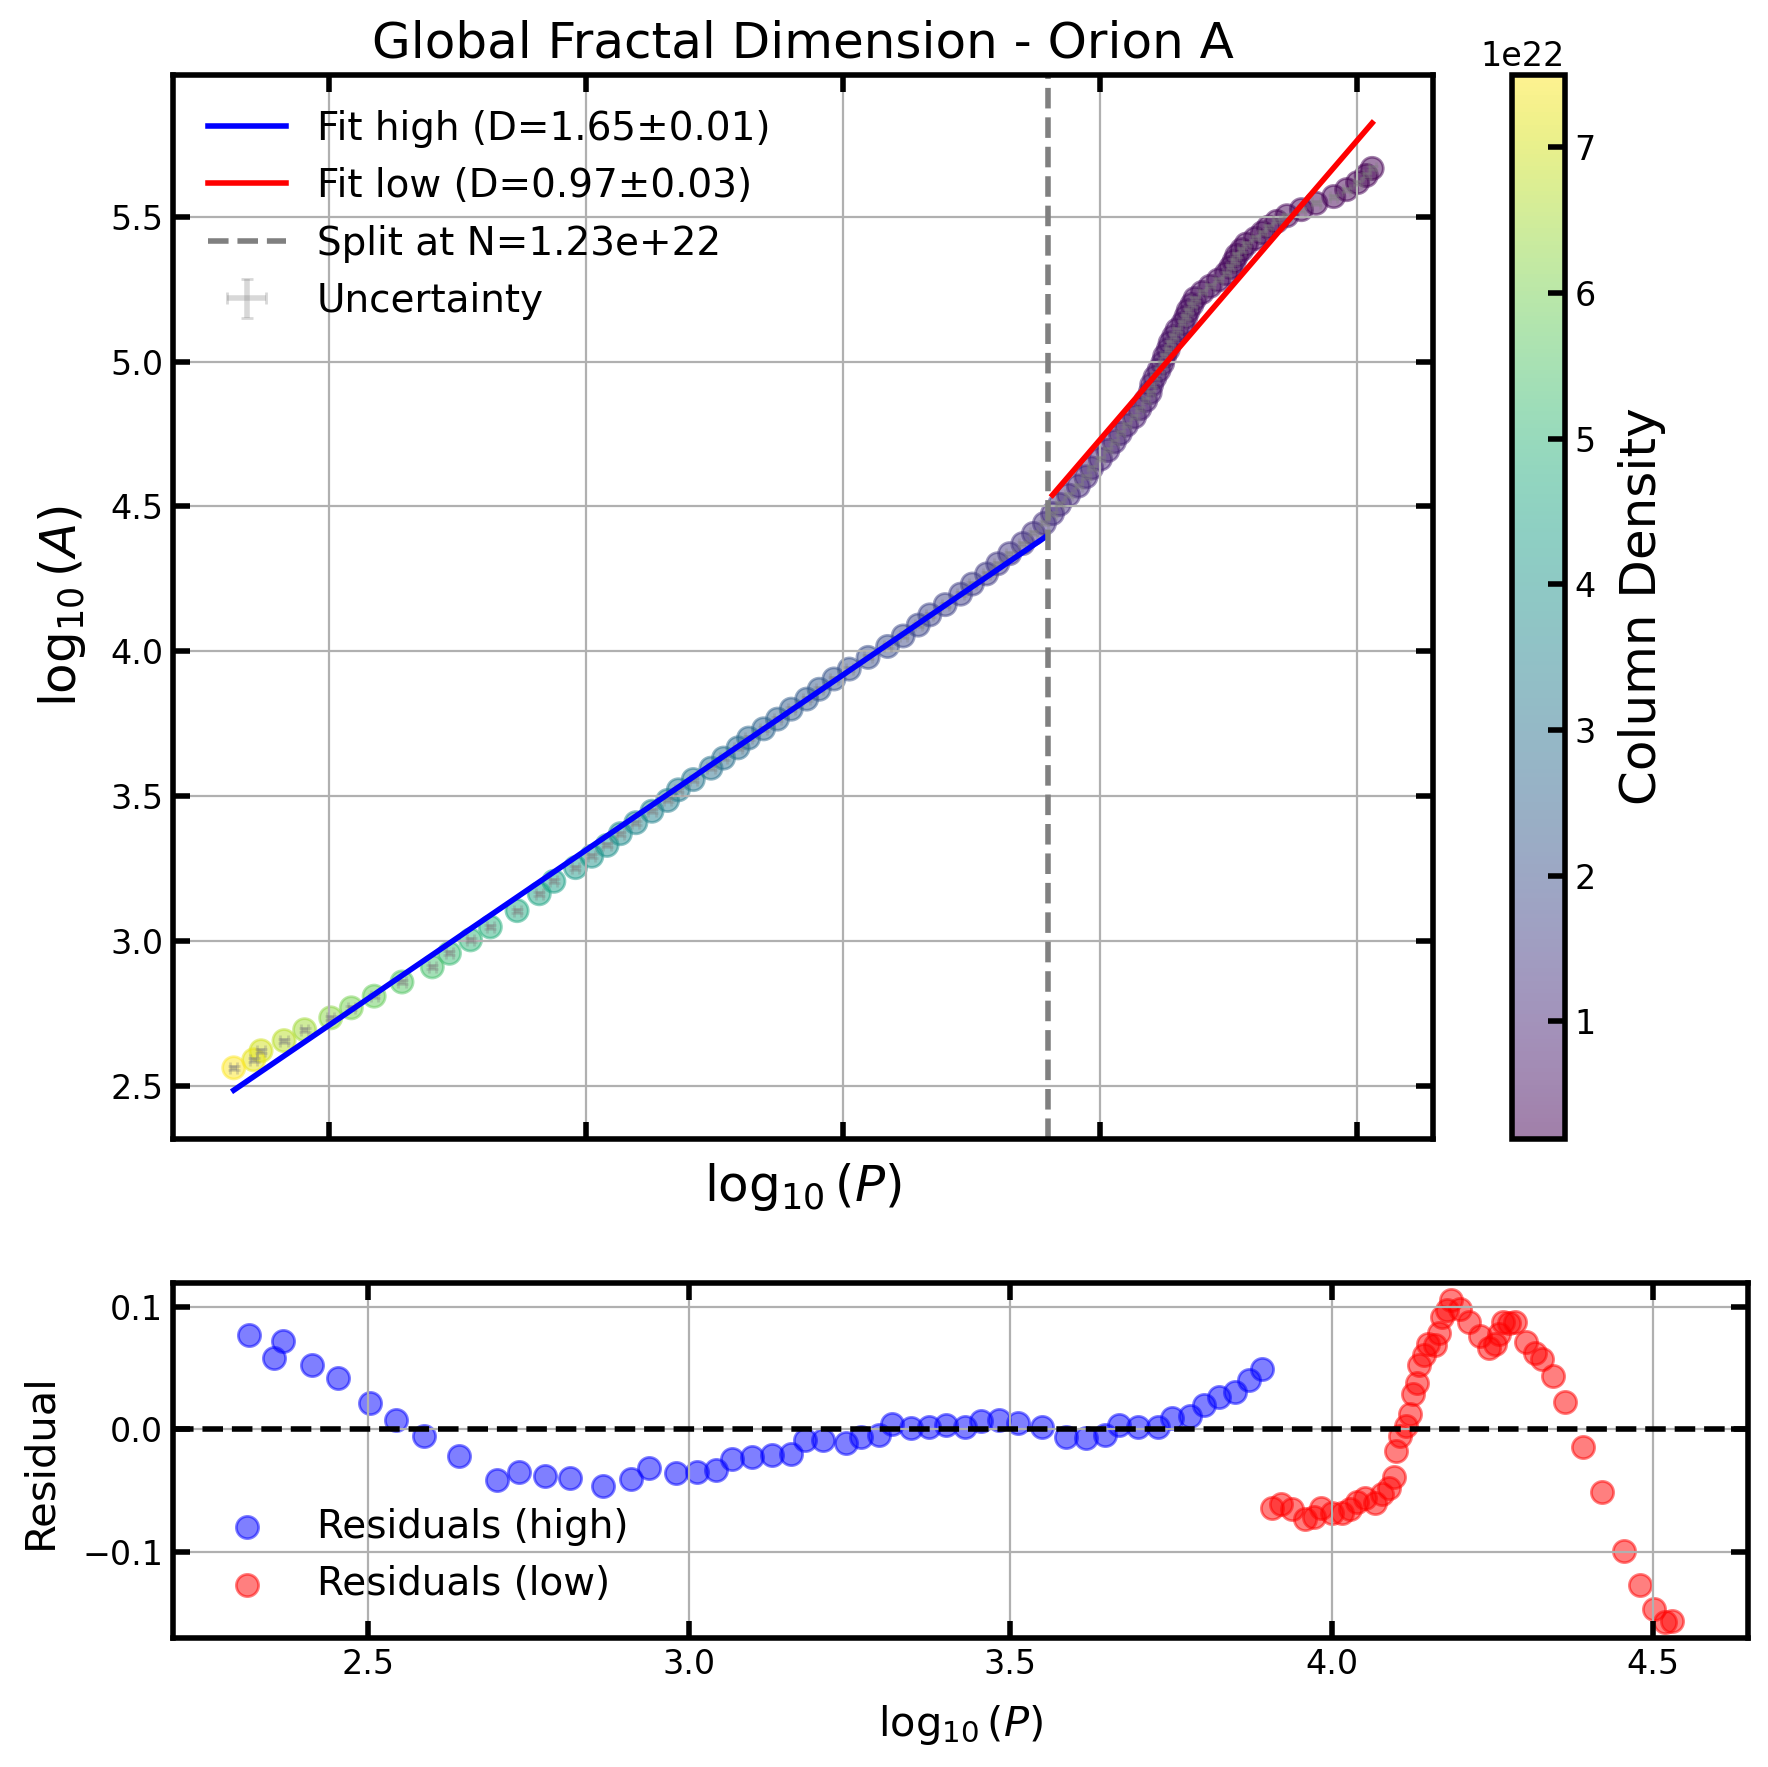
\includegraphics[width=0.5\textwidth]{figures/orion_A_global_double_fit.png}
    \caption{Perimeter-area relation for Orion A with a segmented linear fit. Dashed lines indicate the two fitted regimes, separated at \(N = 1.23 \times 10^{22}\,\mathrm{cm}^{-2}\). Residuals are shown in the lower panel.}
    \label{fig:orion_A_global_double_fit}
\end{figure}

In contrast, Orion B exhibits a well-behaved perimeter-area relation that is accurately described by a single linear fit across the entire column-density range:
\[
D_{\mathrm{OB,\,Global}} = 1.40 \pm 0.01 .
\]
The corresponding residuals (mean absolute residual = 0.0493) and correlation coefficient (0.9976) confirm the robustness of this fit. Figure \ref{fig:orion_B_global} shows the fitted relation and residuals. The consistency of the slope across scales indicates a more uniform degree of structural complexity compared to Orion~A.

\begin{figure}[t]
    \centering
    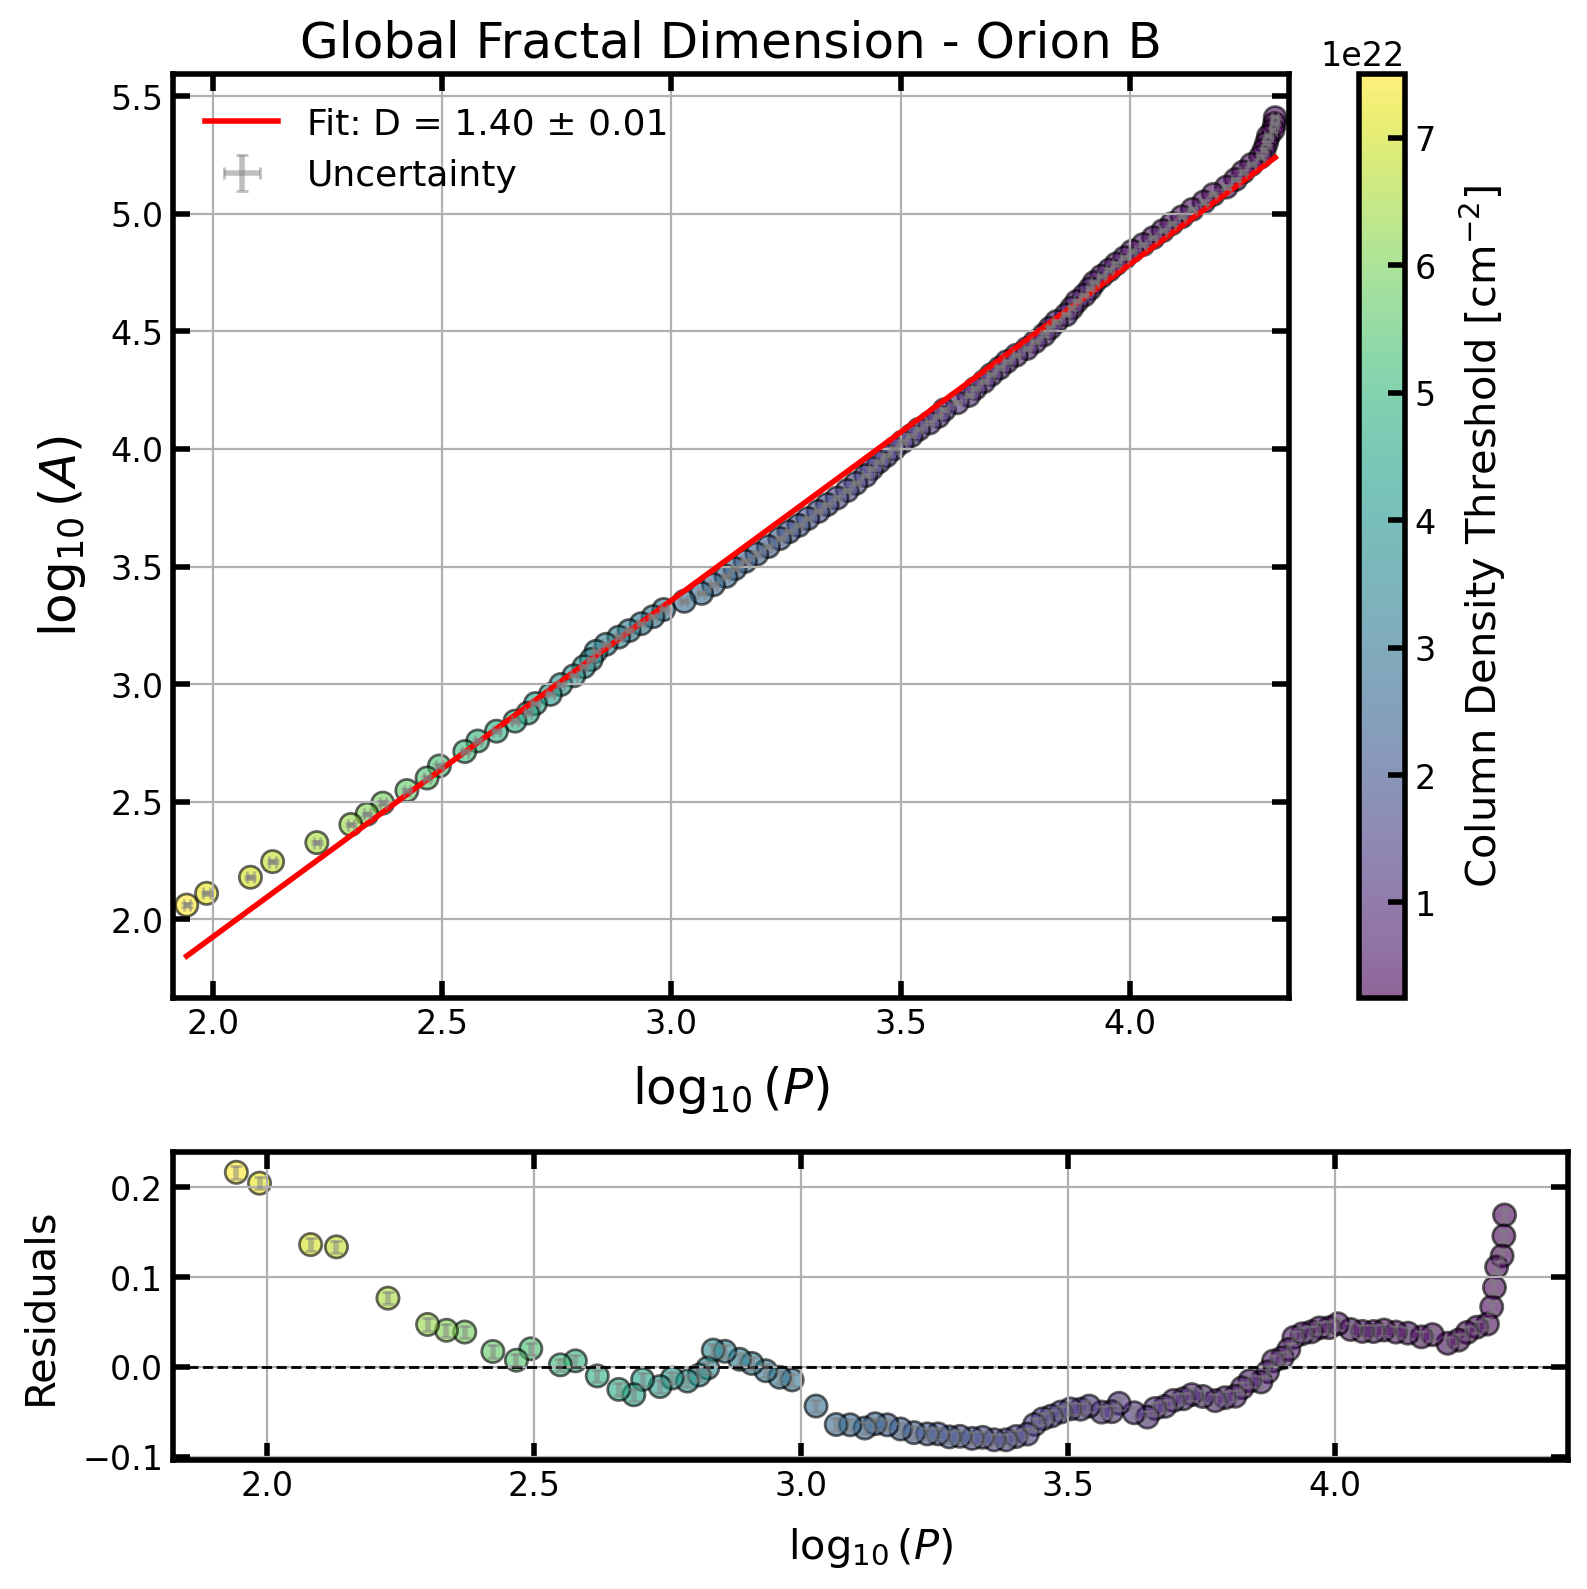
\includegraphics[width=0.5\textwidth]{figures/orion_B_global.png}
    \caption{Perimeter-area relation for Orion~B with the best-fit linear regression overlaid. Residuals are shown in the lower panel.}
    \label{fig:orion_B_global}
\end{figure}

The uncertainties in perimeter and area measurements were estimated at 1.6\%, based on simulations demonstrating that this level of error is representative across different reference geometries.

\section{Local Properties}

\subsection{Euler Characteristic}

We evaluated the Euler characteristic, \(\chi\), for both Orion A and Orion B as a function of the column–density threshold. This topological descriptor quantifies the connectivity and fragmentation of structures within the clouds: negative values of \(\chi\) indicate a predominance of isolated regions, while more positive values reflect a higher degree of connectivity.

Figures~\ref{fig:Euler_Orion_A_no_figs} and~\ref{fig:Euler_Orion_B_no_figs} present the results for Orion A and Orion B, respectively. In both cases of Orion A and B, \(\chi\) was computed over the same range of column densities \(N_\mathrm{min} \leq N \leq N_\mathrm{max}\) used in the gloabl perimeter–area analysis above, ensuring consistency and comparability.

\begin{figure}[t]
    \centering
    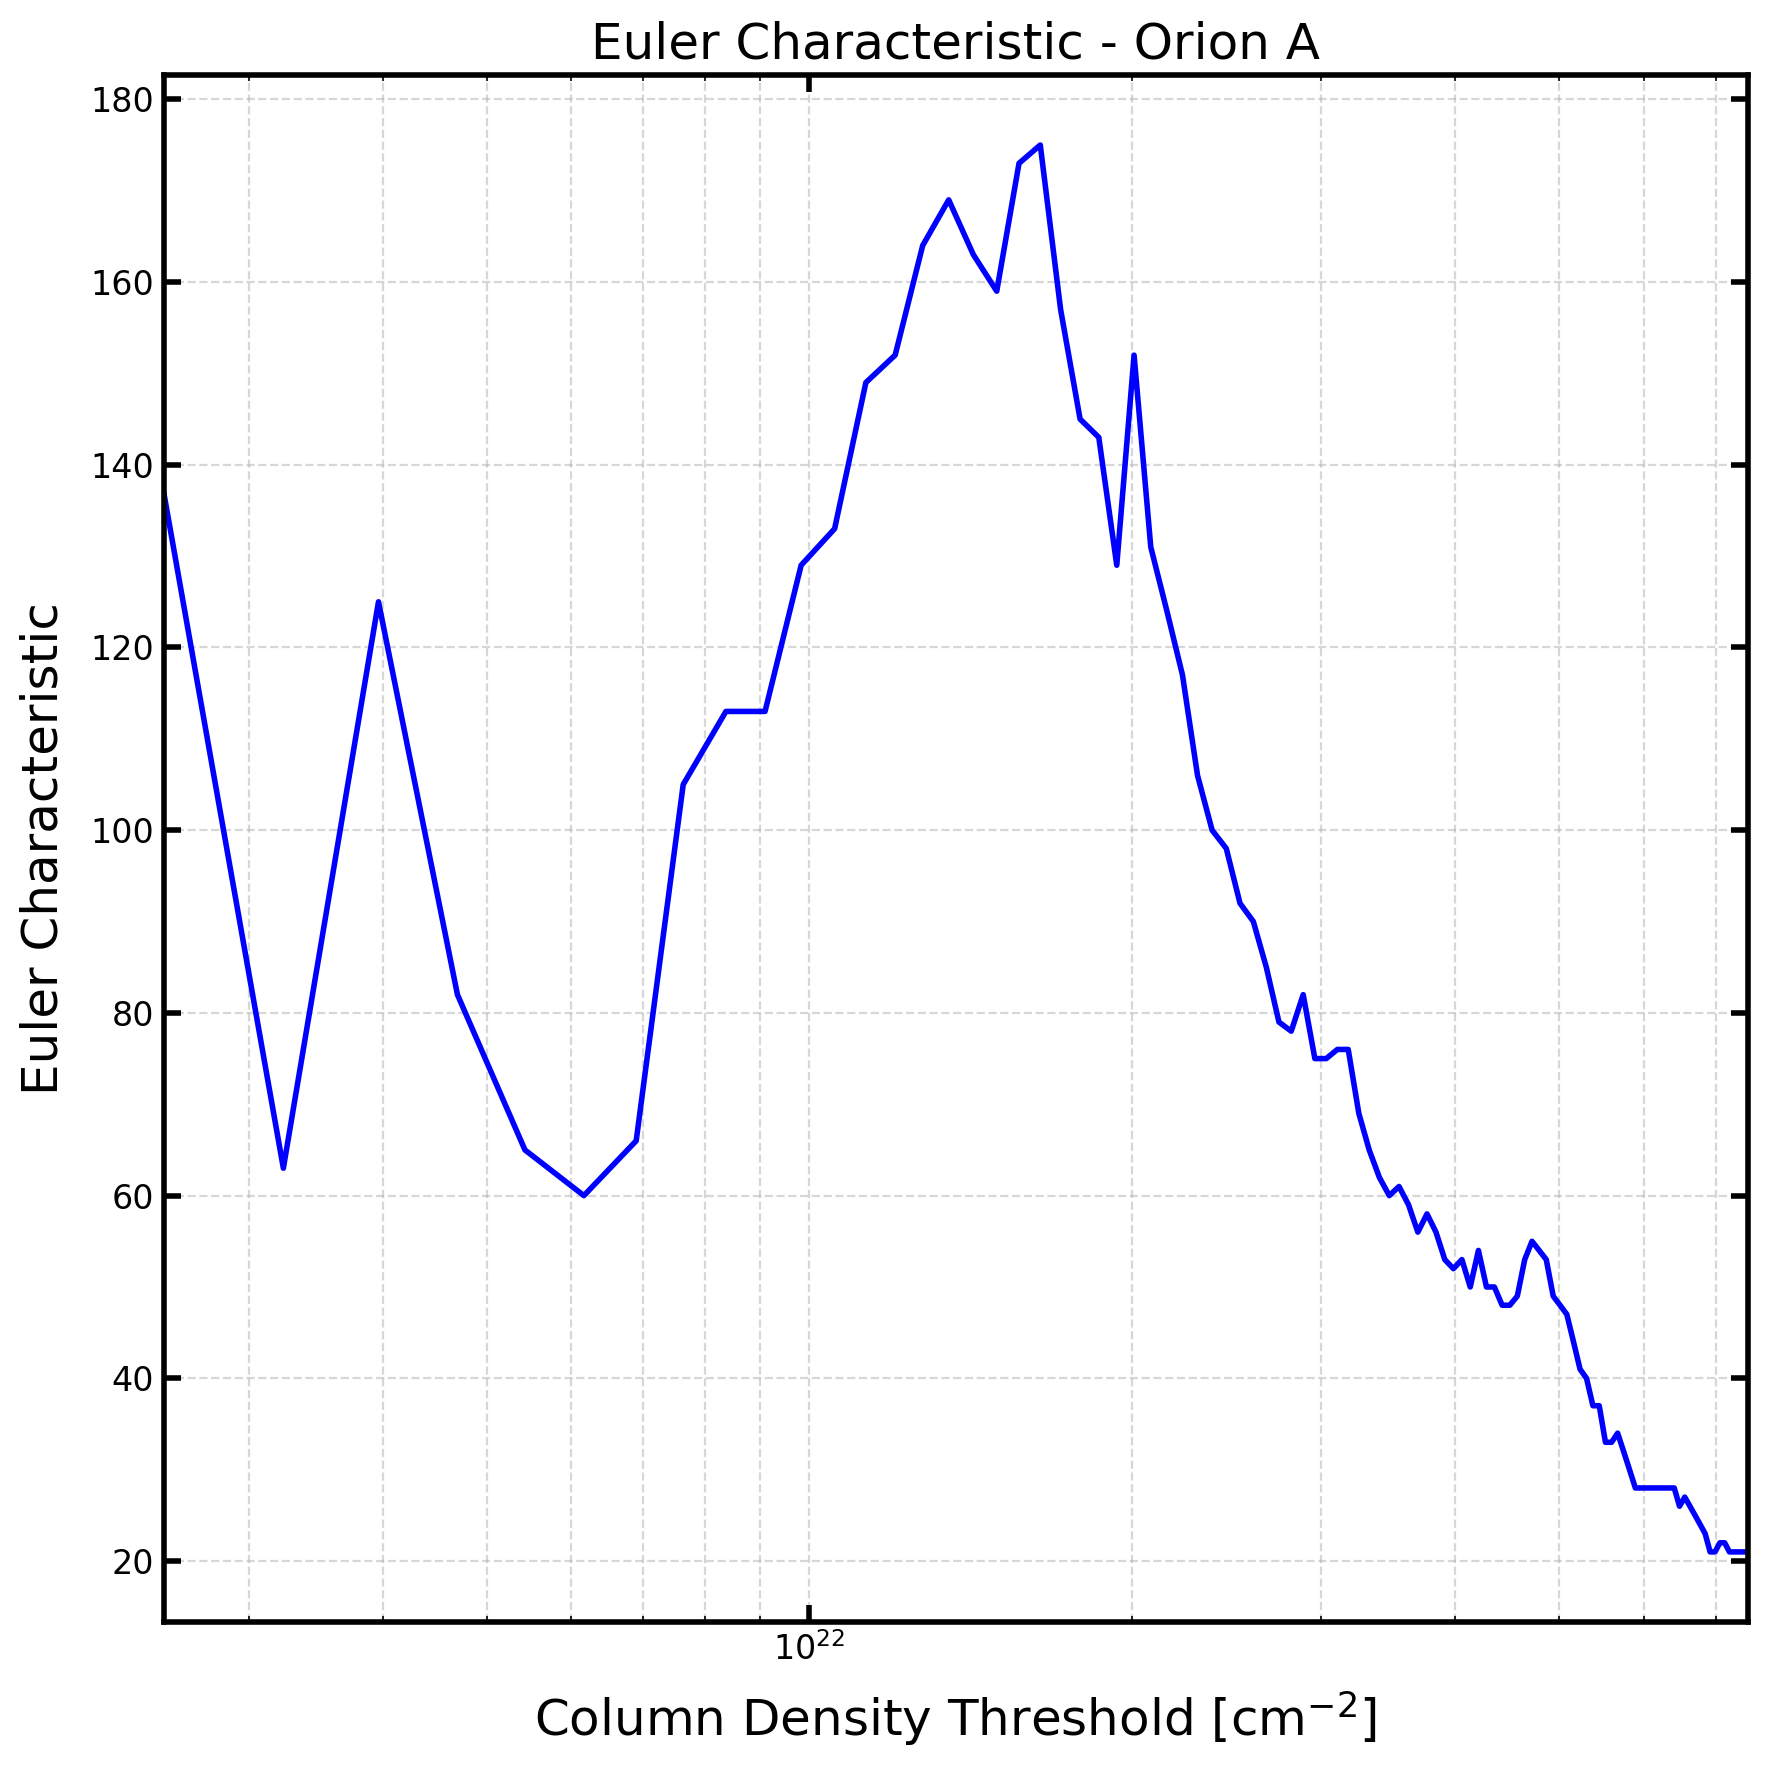
\includegraphics[width=0.45\textwidth]{figures/euler_Orion_A_no_figs.png}
    \caption{Euler characteristic of Orion A as a function of column–density threshold. Positive values correspond to a predominance of isolated structures, while negative values indicate higher connectivity.}
    \label{fig:Euler_Orion_A_no_figs}
\end{figure}

\begin{figure}[t]
    \centering
    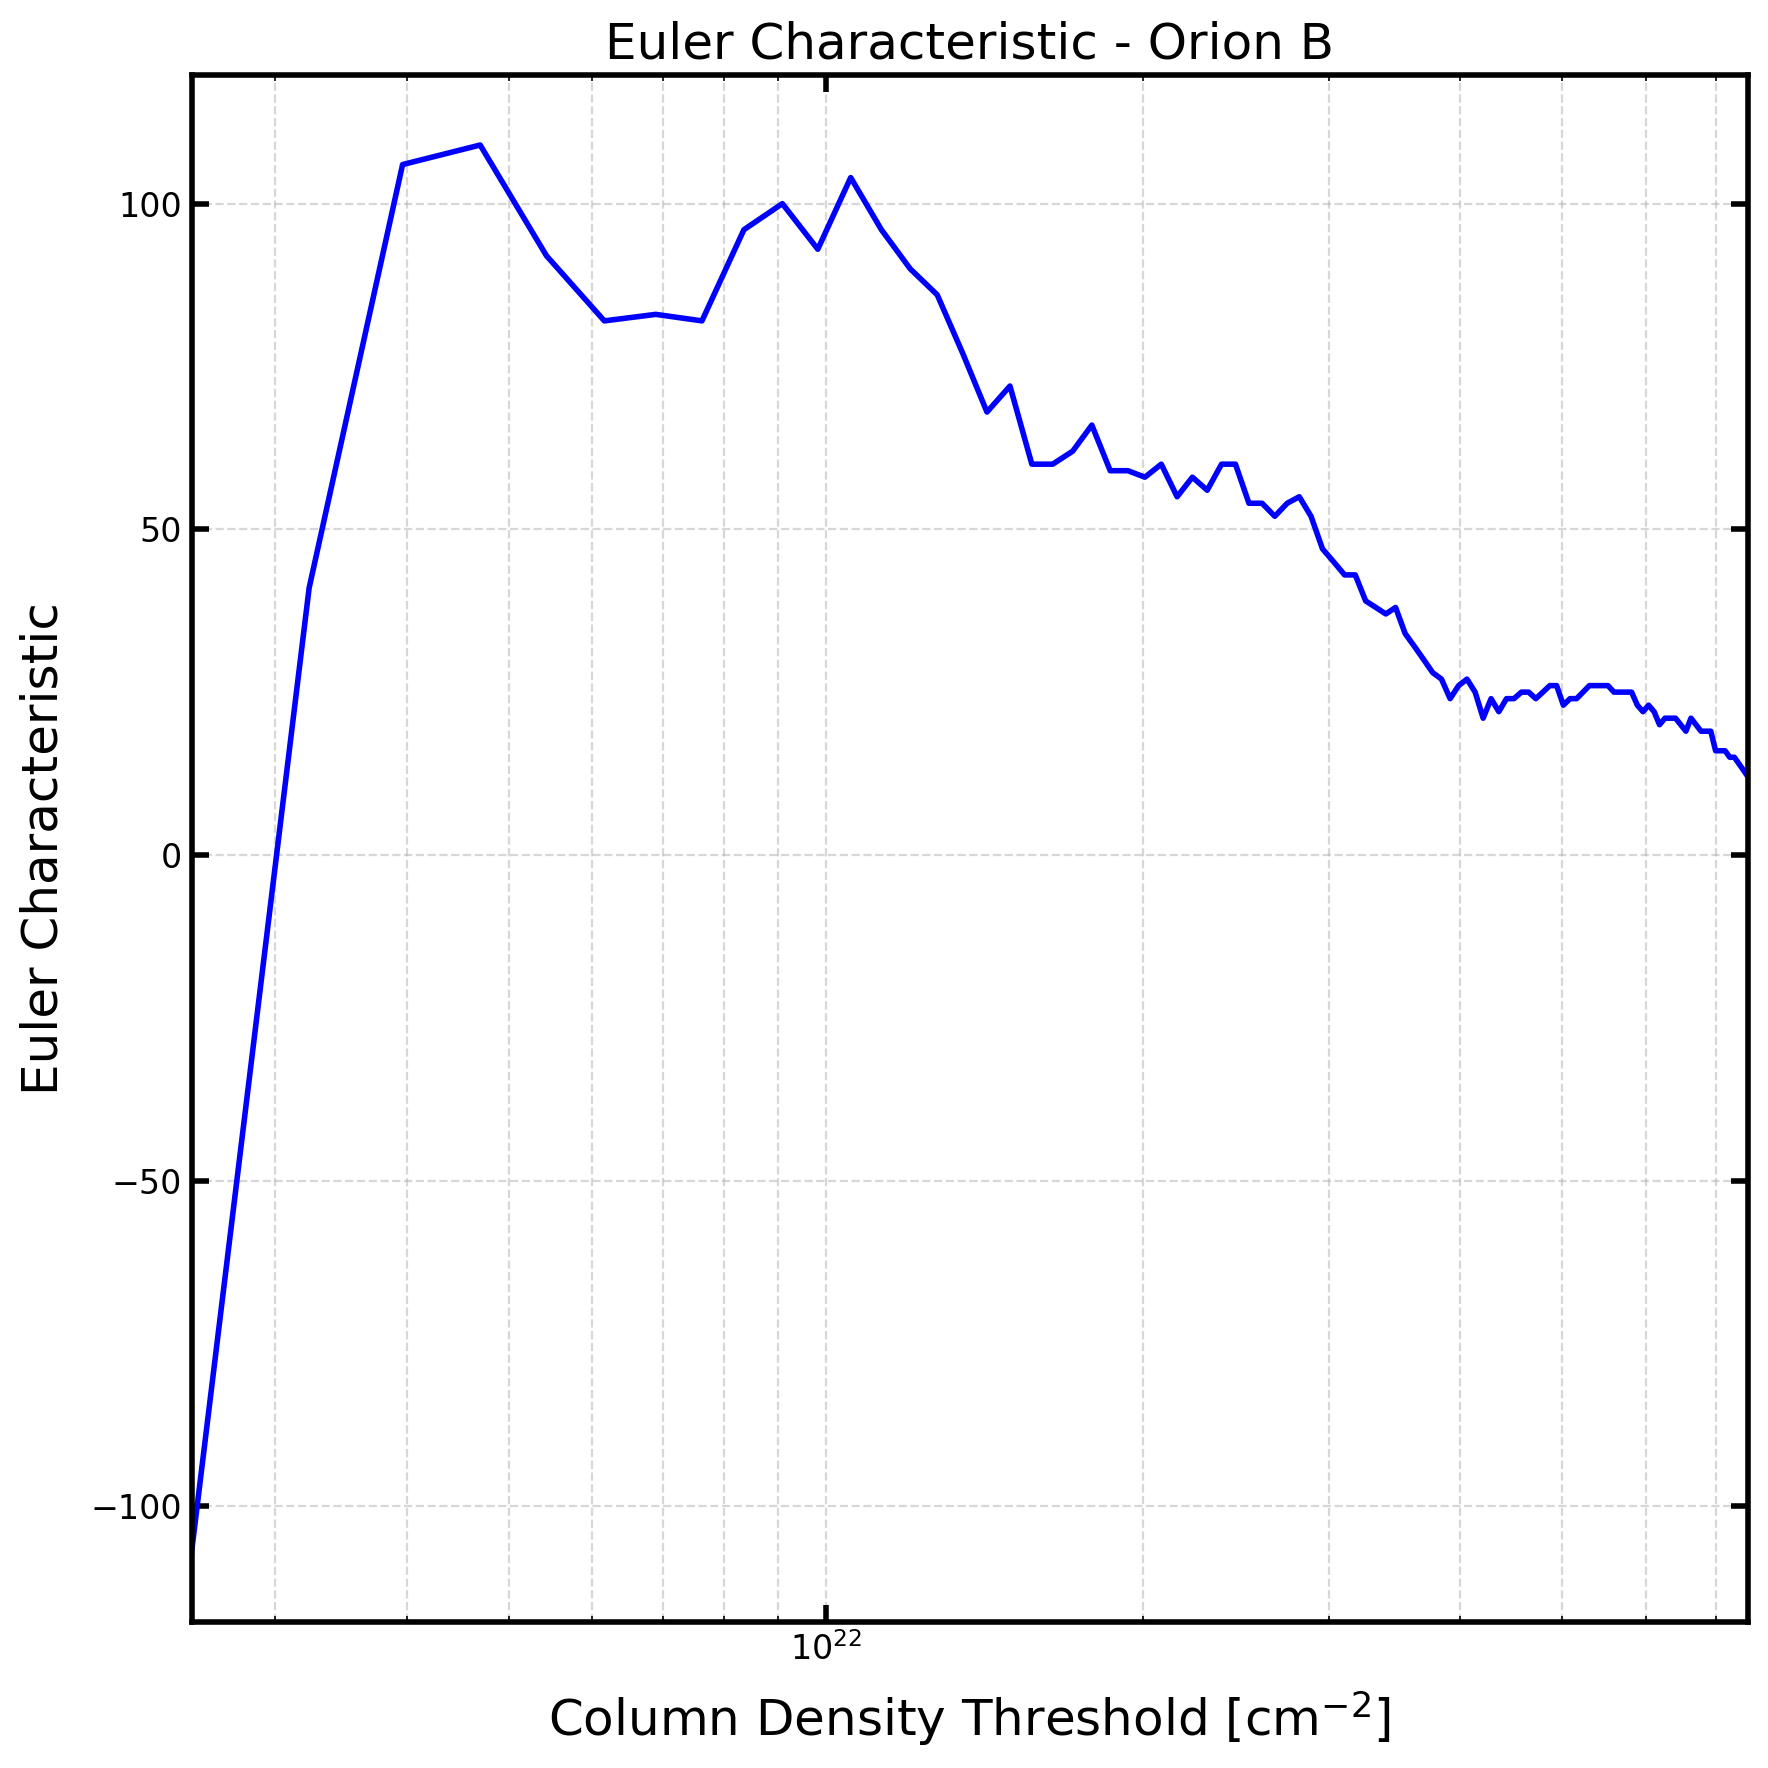
\includegraphics[width=0.45\textwidth]{figures/euler_Orion_B_no_figs.png}
    \caption{Euler characteristic of Orion~B as a function of column–density threshold.}
    \label{fig:Euler_Orion_B_no_figs}
\end{figure}

Orion A exhibits a profile that closely resembles the Gaussian‑like behavior expected from Gaussian Random Field simulations (Figure \ref{fig:sims_euler_char}), with a pronounced peak at approximately $1.64 \times 10^{22} \,\mathrm{cm}^{-2}$. In contrast, Orion B shows a more linear trend. In both regions, strong numerical fluctuations appear at lower column-density thresholds, leading to noticeable variations in the calculated Euler characteristic.

\subsection{Local Fractal Dimension}

Figure~\ref{fig:local_Orion_A_B} shows the variation of the local fractal dimension $D(\nu)$ as a function of column-density threshold for Orion A and Orion B. The column density range  \(N_\mathrm{min} \leq N \leq N_\mathrm{max}\) is the same as in the previous sections. In both regions we find a clear overall trend: the local fractal dimension changes systematically as the threshold increases. Superimposed on this trend, several pronounced peaks and deviations are visible. These features likely trace transitions in the morphology of the structures, for instance the emergence of compact cores or the fragmentation of filaments into smaller substructures.

A more detailed interpretation of these peaks and their implications for cloud evolution and turbulence will be addressed in the following section.

\begin{figure}[t]
    \centering
    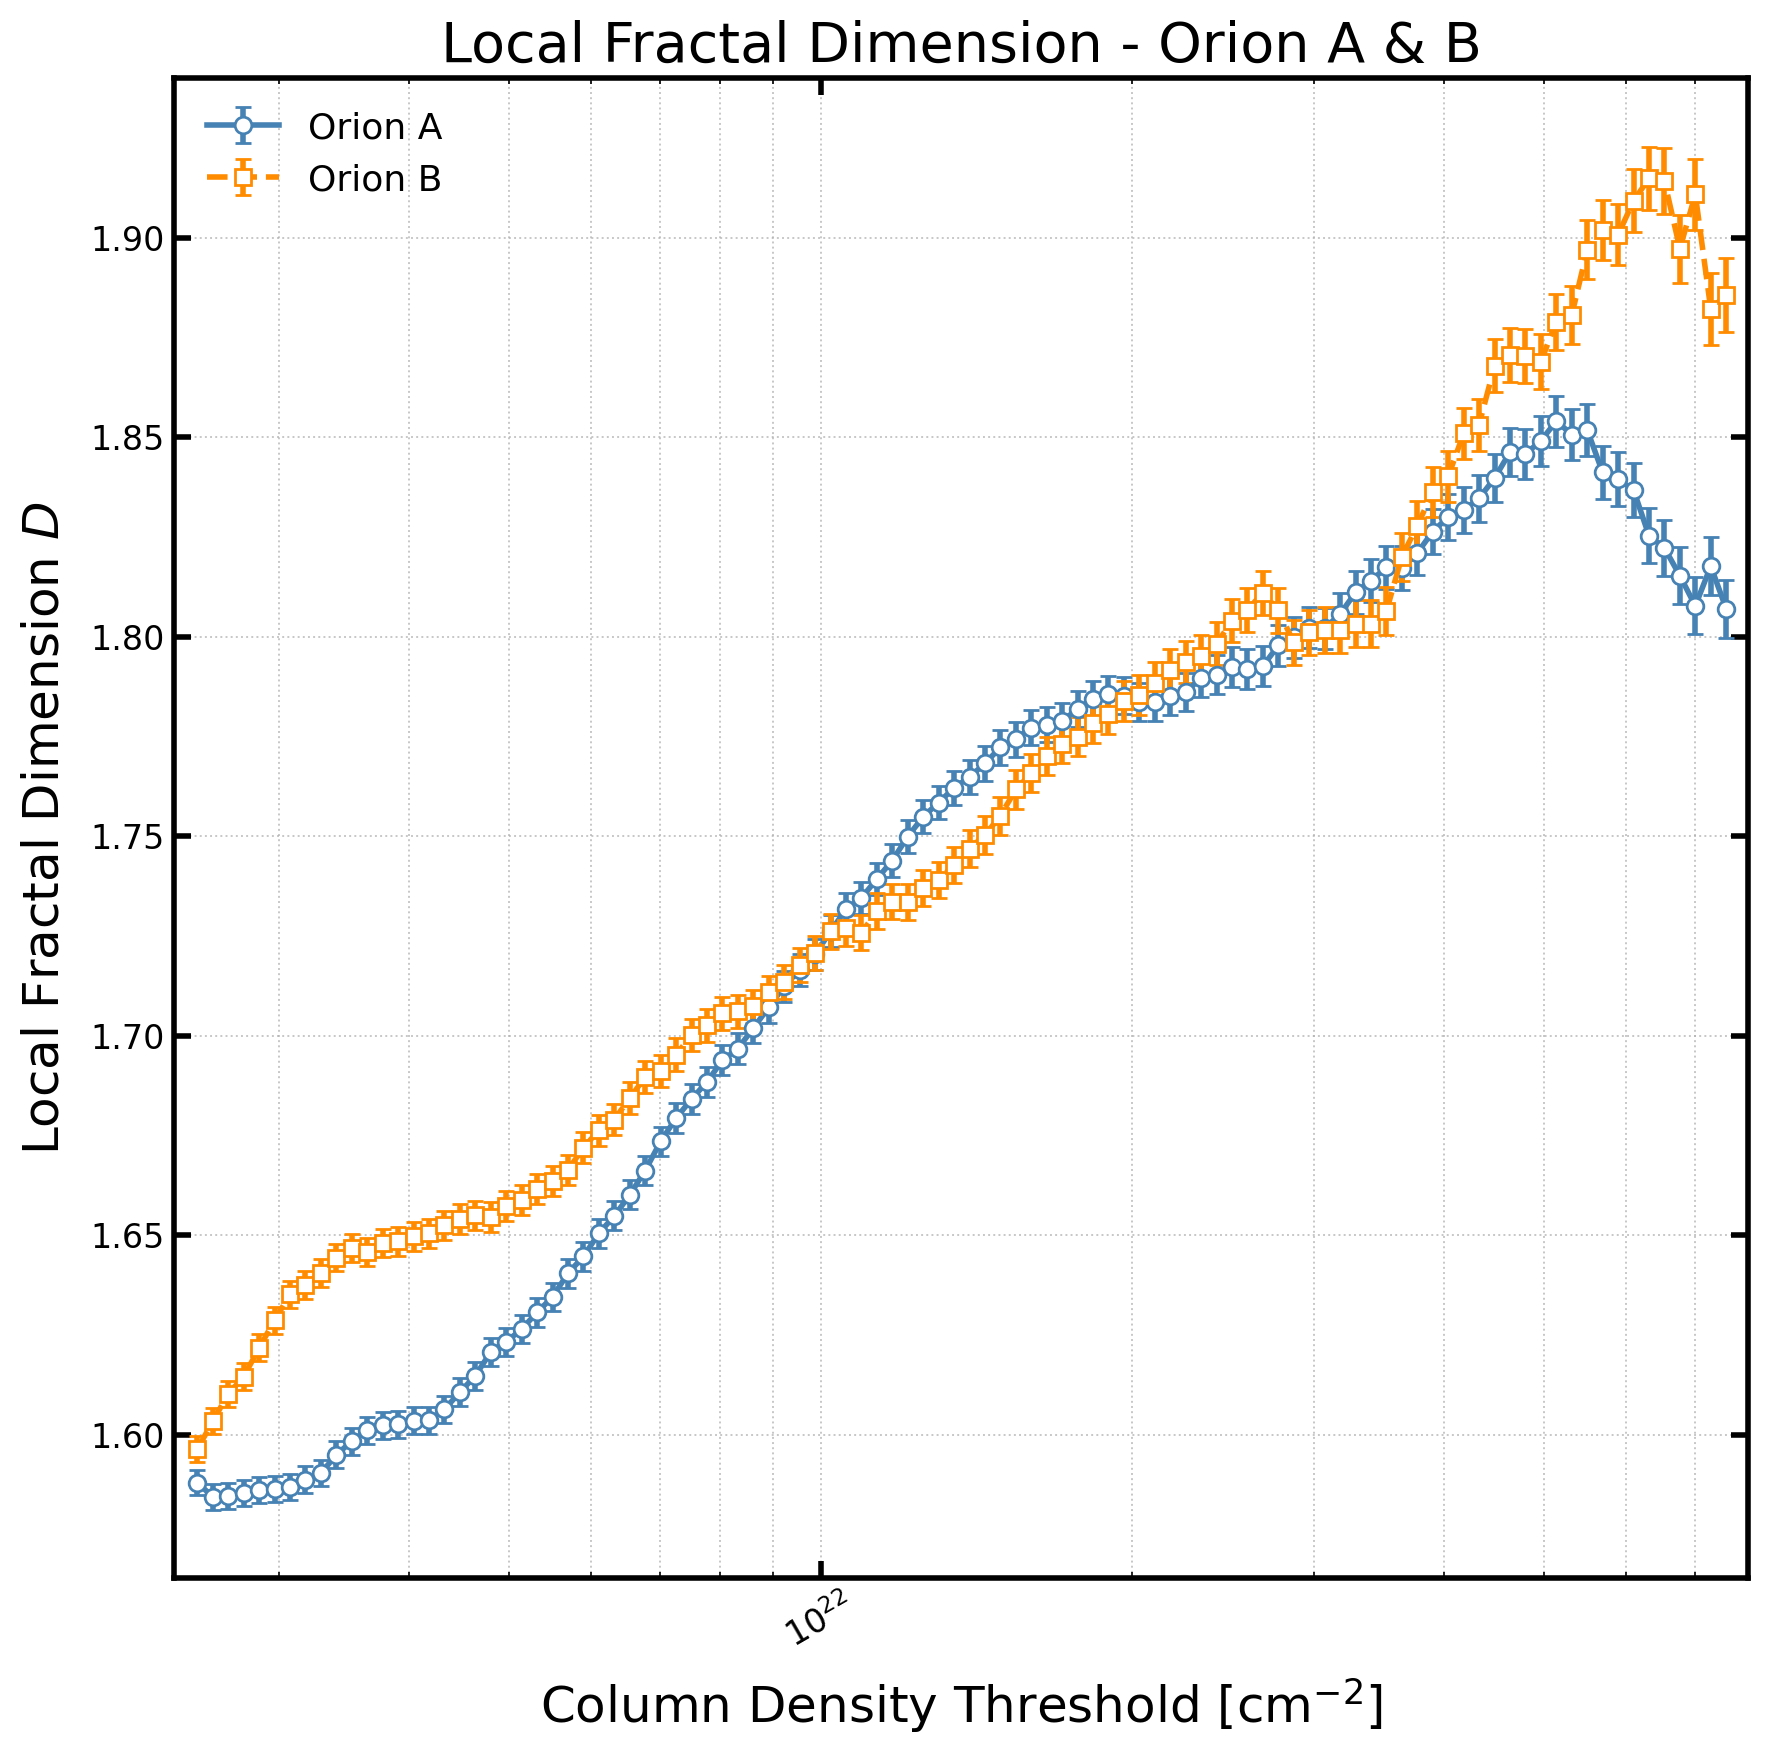
\includegraphics[width=0.5\textwidth]{figures/local_orion_A_B.png}
    \caption{Local fractal dimension as a function of column-density threshold for Orion A and Orion B. Error bars reflect the uncertainties of the fit at each threshold.}
    \label{fig:local_Orion_A_B}
\end{figure}

The average values and their standard deviations of the local fractal dimension for the two regions are:
\[
\bar{D}_{\mathrm{OA,\,Local}} = 1.73 \pm 0.09,
\]
\[
\bar{D}_{\mathrm{OB,\,Local}} = 1.75 \pm 0.08.
\]

The uncertainties in perimeter and area measurements were estimated again at approximately 1.6\%, based on simulation results.

% To-Do:
% add uncertainties
% make graphs more similar to local Orion A and B
% add average values 
\subsection{Analysis of Individual Structures}

To gain deeper insight into the fractal properties of each cloud, we decomposed the emission at every column-density threshold into its set of connected structures. This dendrogram-based approach provides a hierarchical view of how the material is organized into nested substructures, enabling a more detailed examination of their geometrical and topological properties.

Figures~\ref{fig:dendrogram_A} and~\ref{fig:dendrogram_B} display the resulting dendrograms for Orion~A and Orion~B. These diagrams trace how individual regions merge into larger complexes as the threshold decreases, effectively capturing the clustering behaviour of the cloud across spatial scales.

\begin{figure}[t]
    \centering
    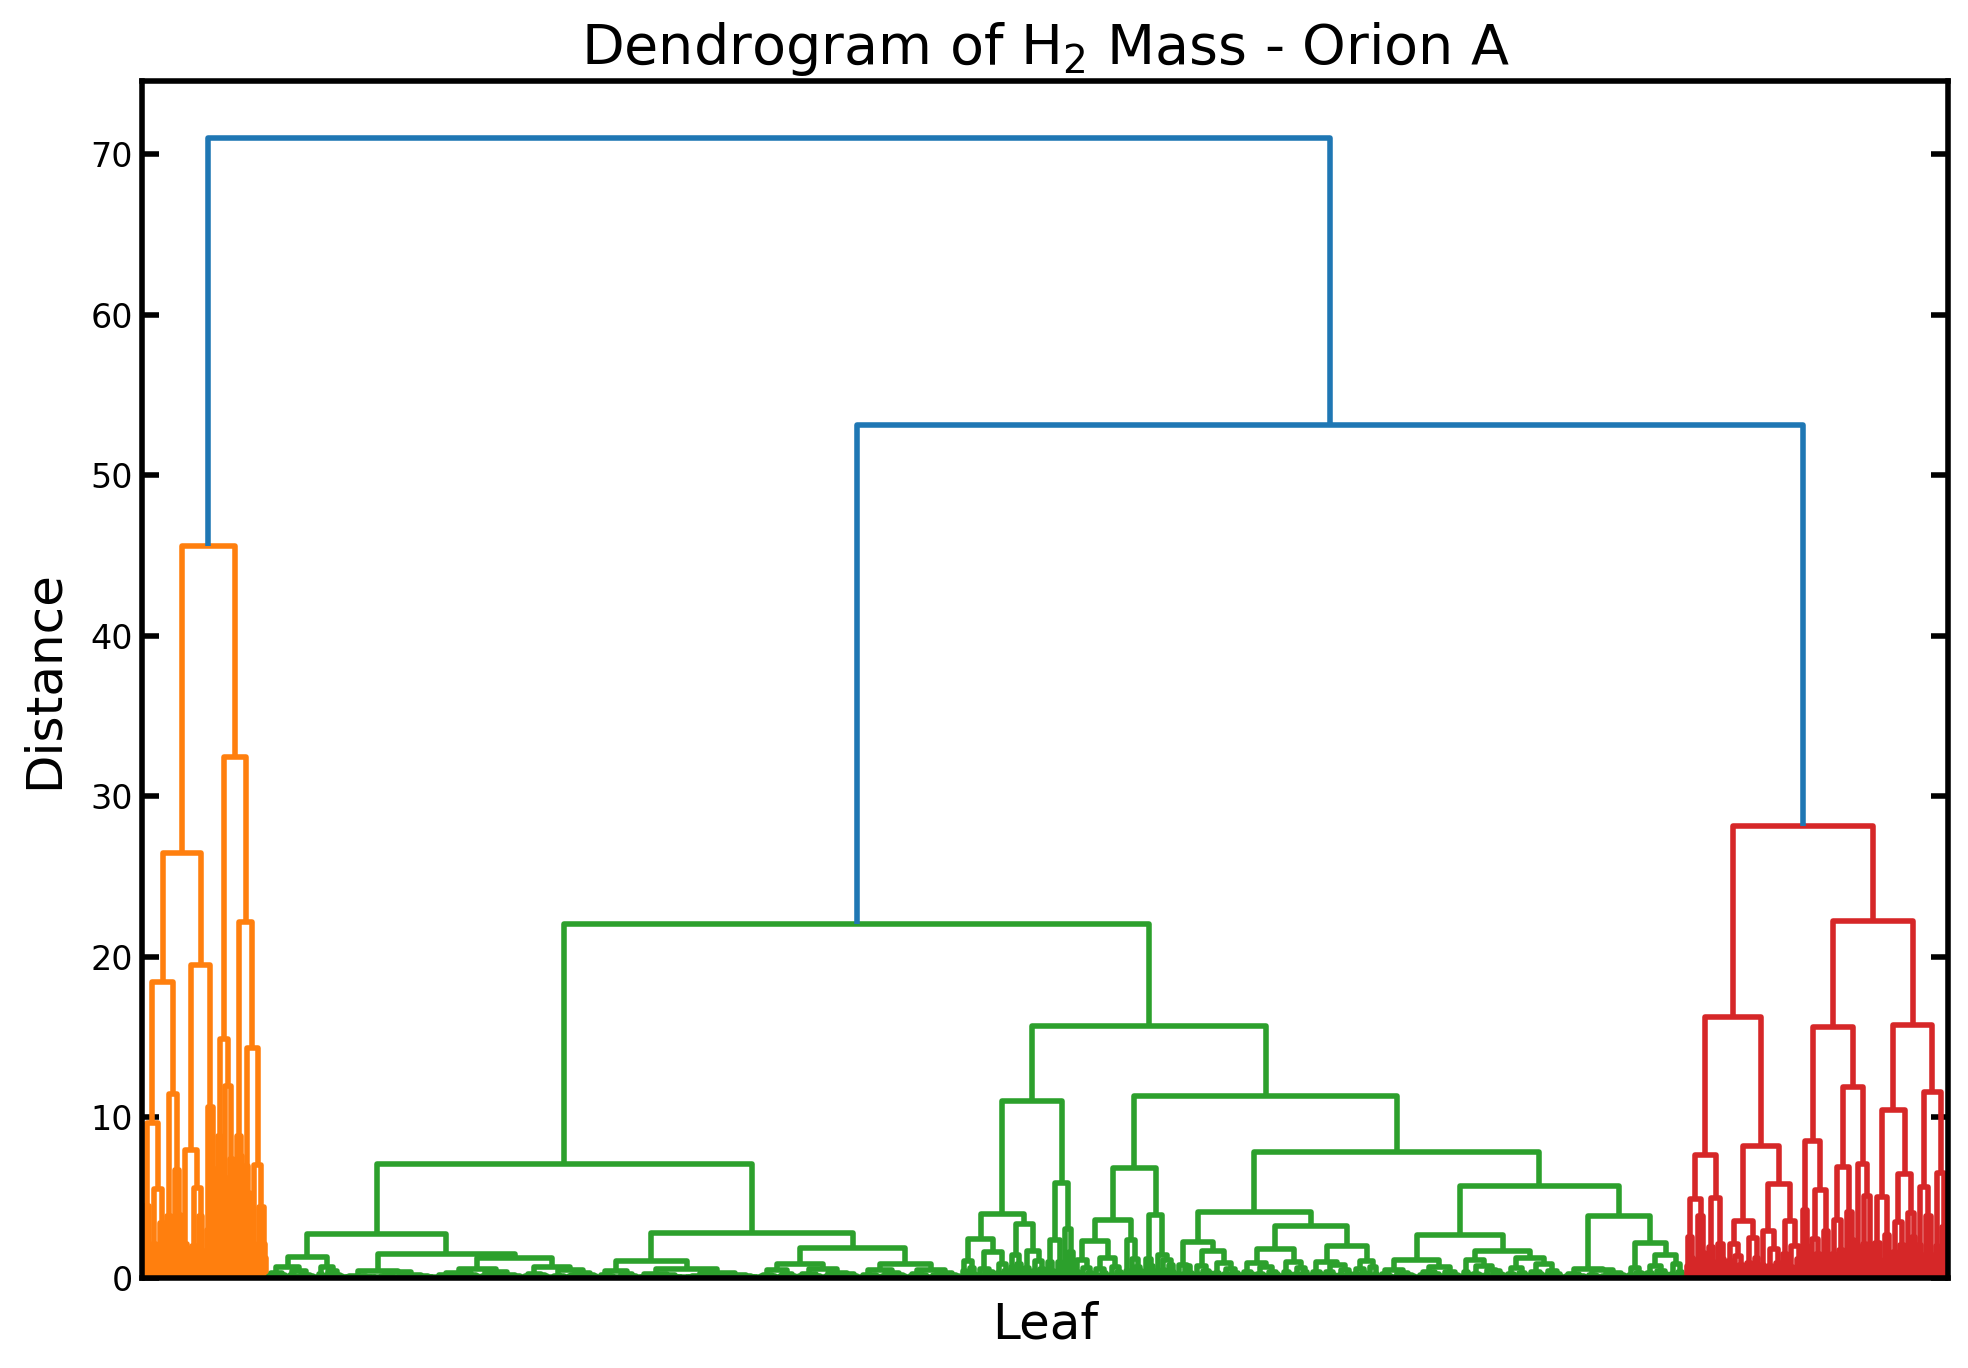
\includegraphics[width=0.5\textwidth]{figures/dendogram_A.png}
    \caption{Dendrogram of the Orion~A mass distribution, showing the hierarchical merging of structures as the column-density threshold is lowered. The various main branches are coloured differently for highlighting purposes. The y-axis "Distance" represents a degree of similarity between structures. }
    \label{fig:dendrogram_A}
\end{figure}

\begin{figure}[t]
    \centering
    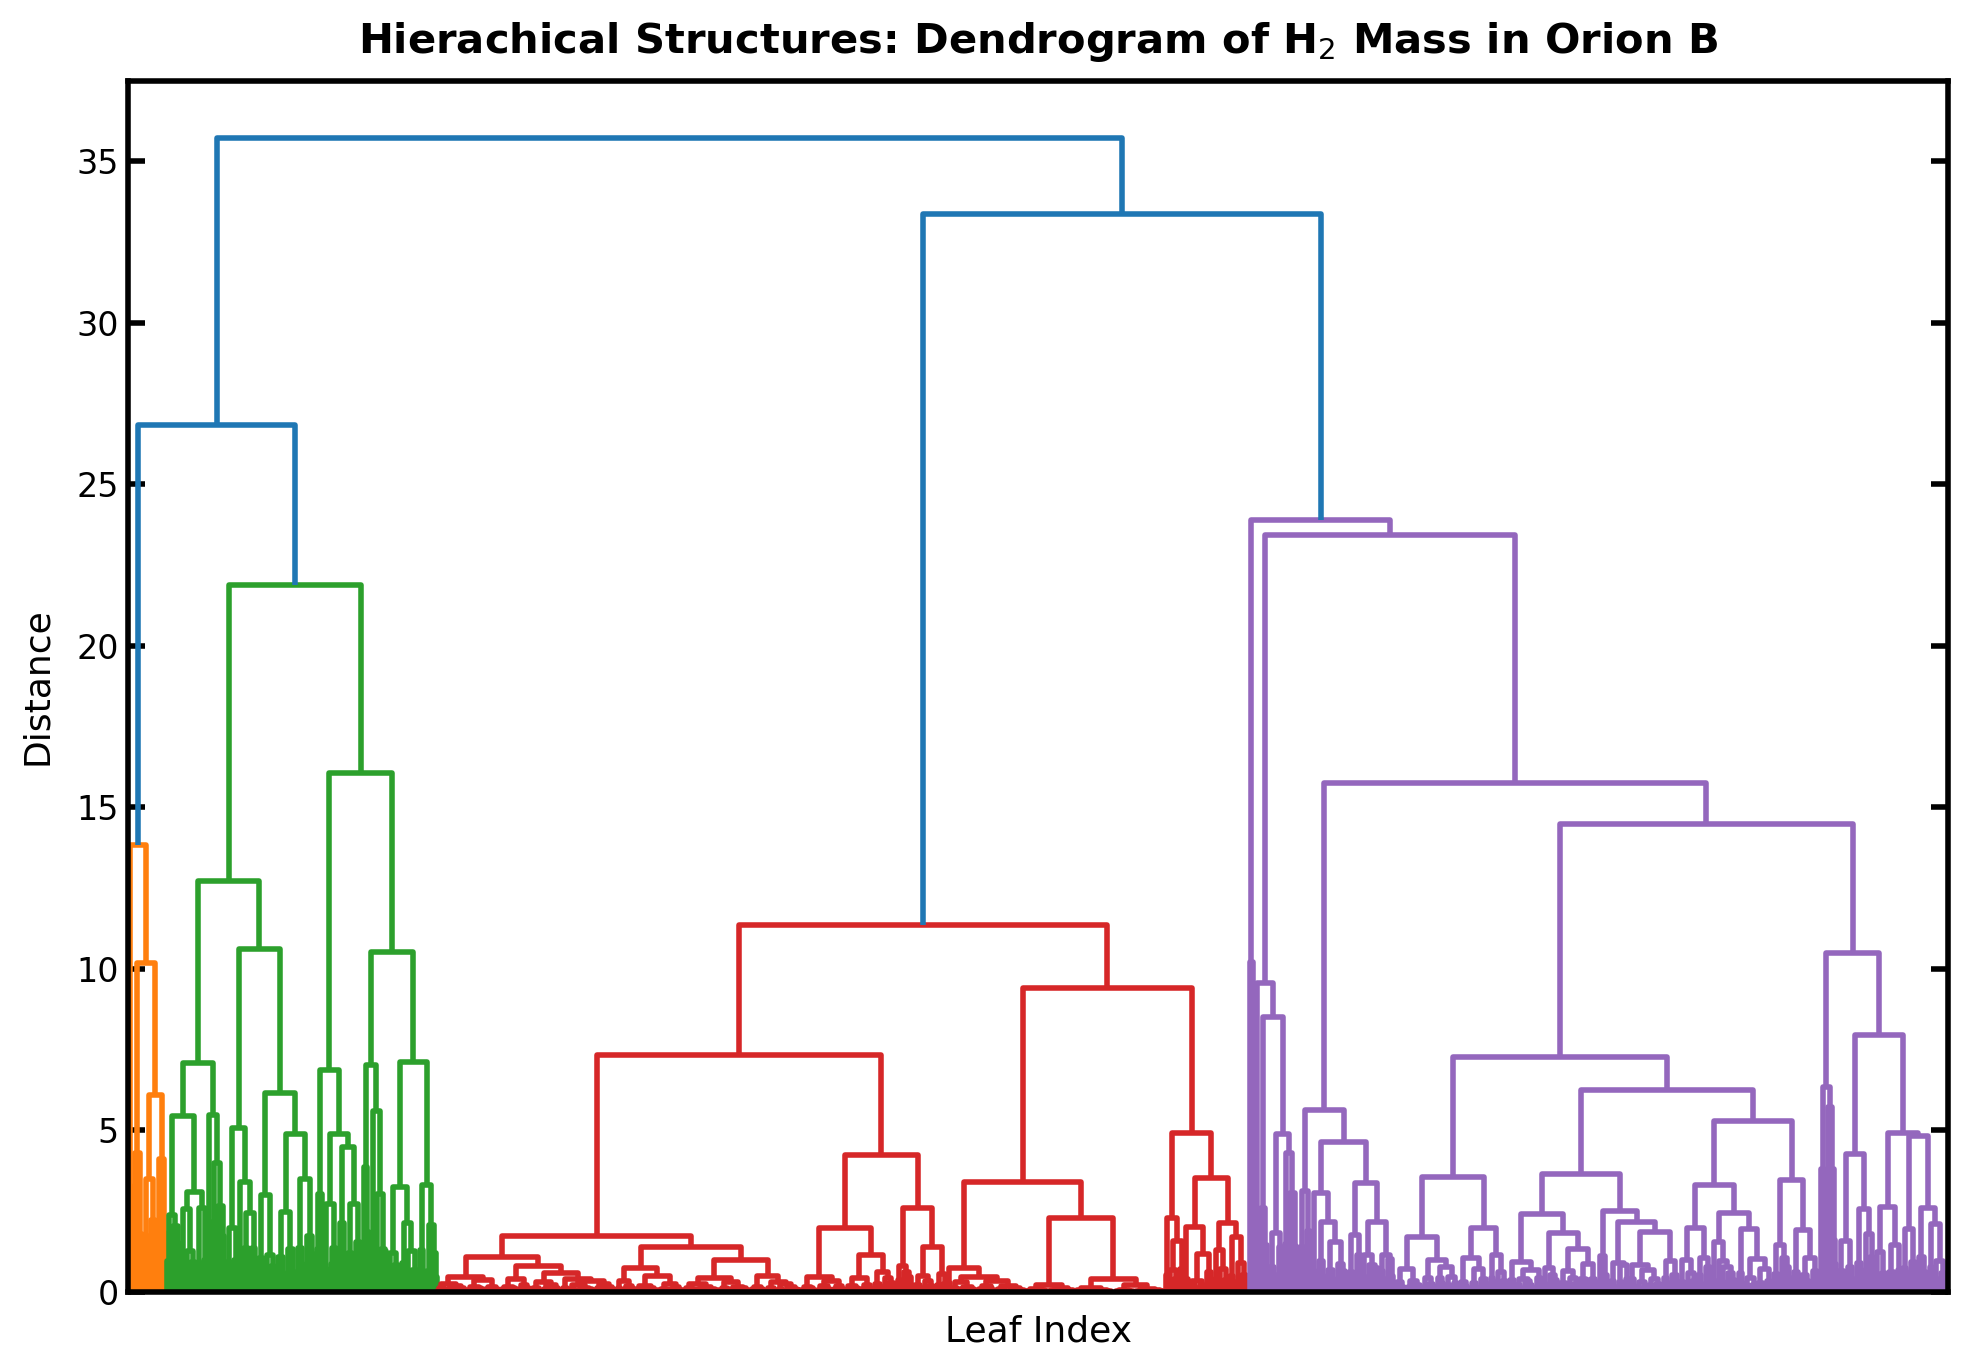
\includegraphics[width=0.5\textwidth]{figures/dendogram_B.png}
    \caption{Dendrogram of the Orion~B mass distribution, showing the hierarchical merging of structures as the column-density threshold is lowered.}
    \label{fig:dendrogram_B}
\end{figure}

We then applied the same calculation of the local fractal dimension to each of these connected structures. For numerical stability, we first limited the analysis to the largest regions at each threshold, selecting them according to minimum perimeter and area criteria. The resulting measurements are shown in Figures~\ref{fig:local_A_single_structures} and~\ref{fig:local_B_single_structures}. Overall, these individual-structure analyses reproduce similar trends to those found in the undifferentiated calculation (Figure~\ref{fig:local_Orion_A_B}), although with shallower progression at higher column density thresholds. 
This behaviour has been recorded in other instances, e.g. when the regions got simply divided into N sharp cuts: the calculated local fractal dimensions show similar trends, but with a shallower progression. The average of these then tends to approach the whole region one.   

\begin{figure}[t]
    \centering
    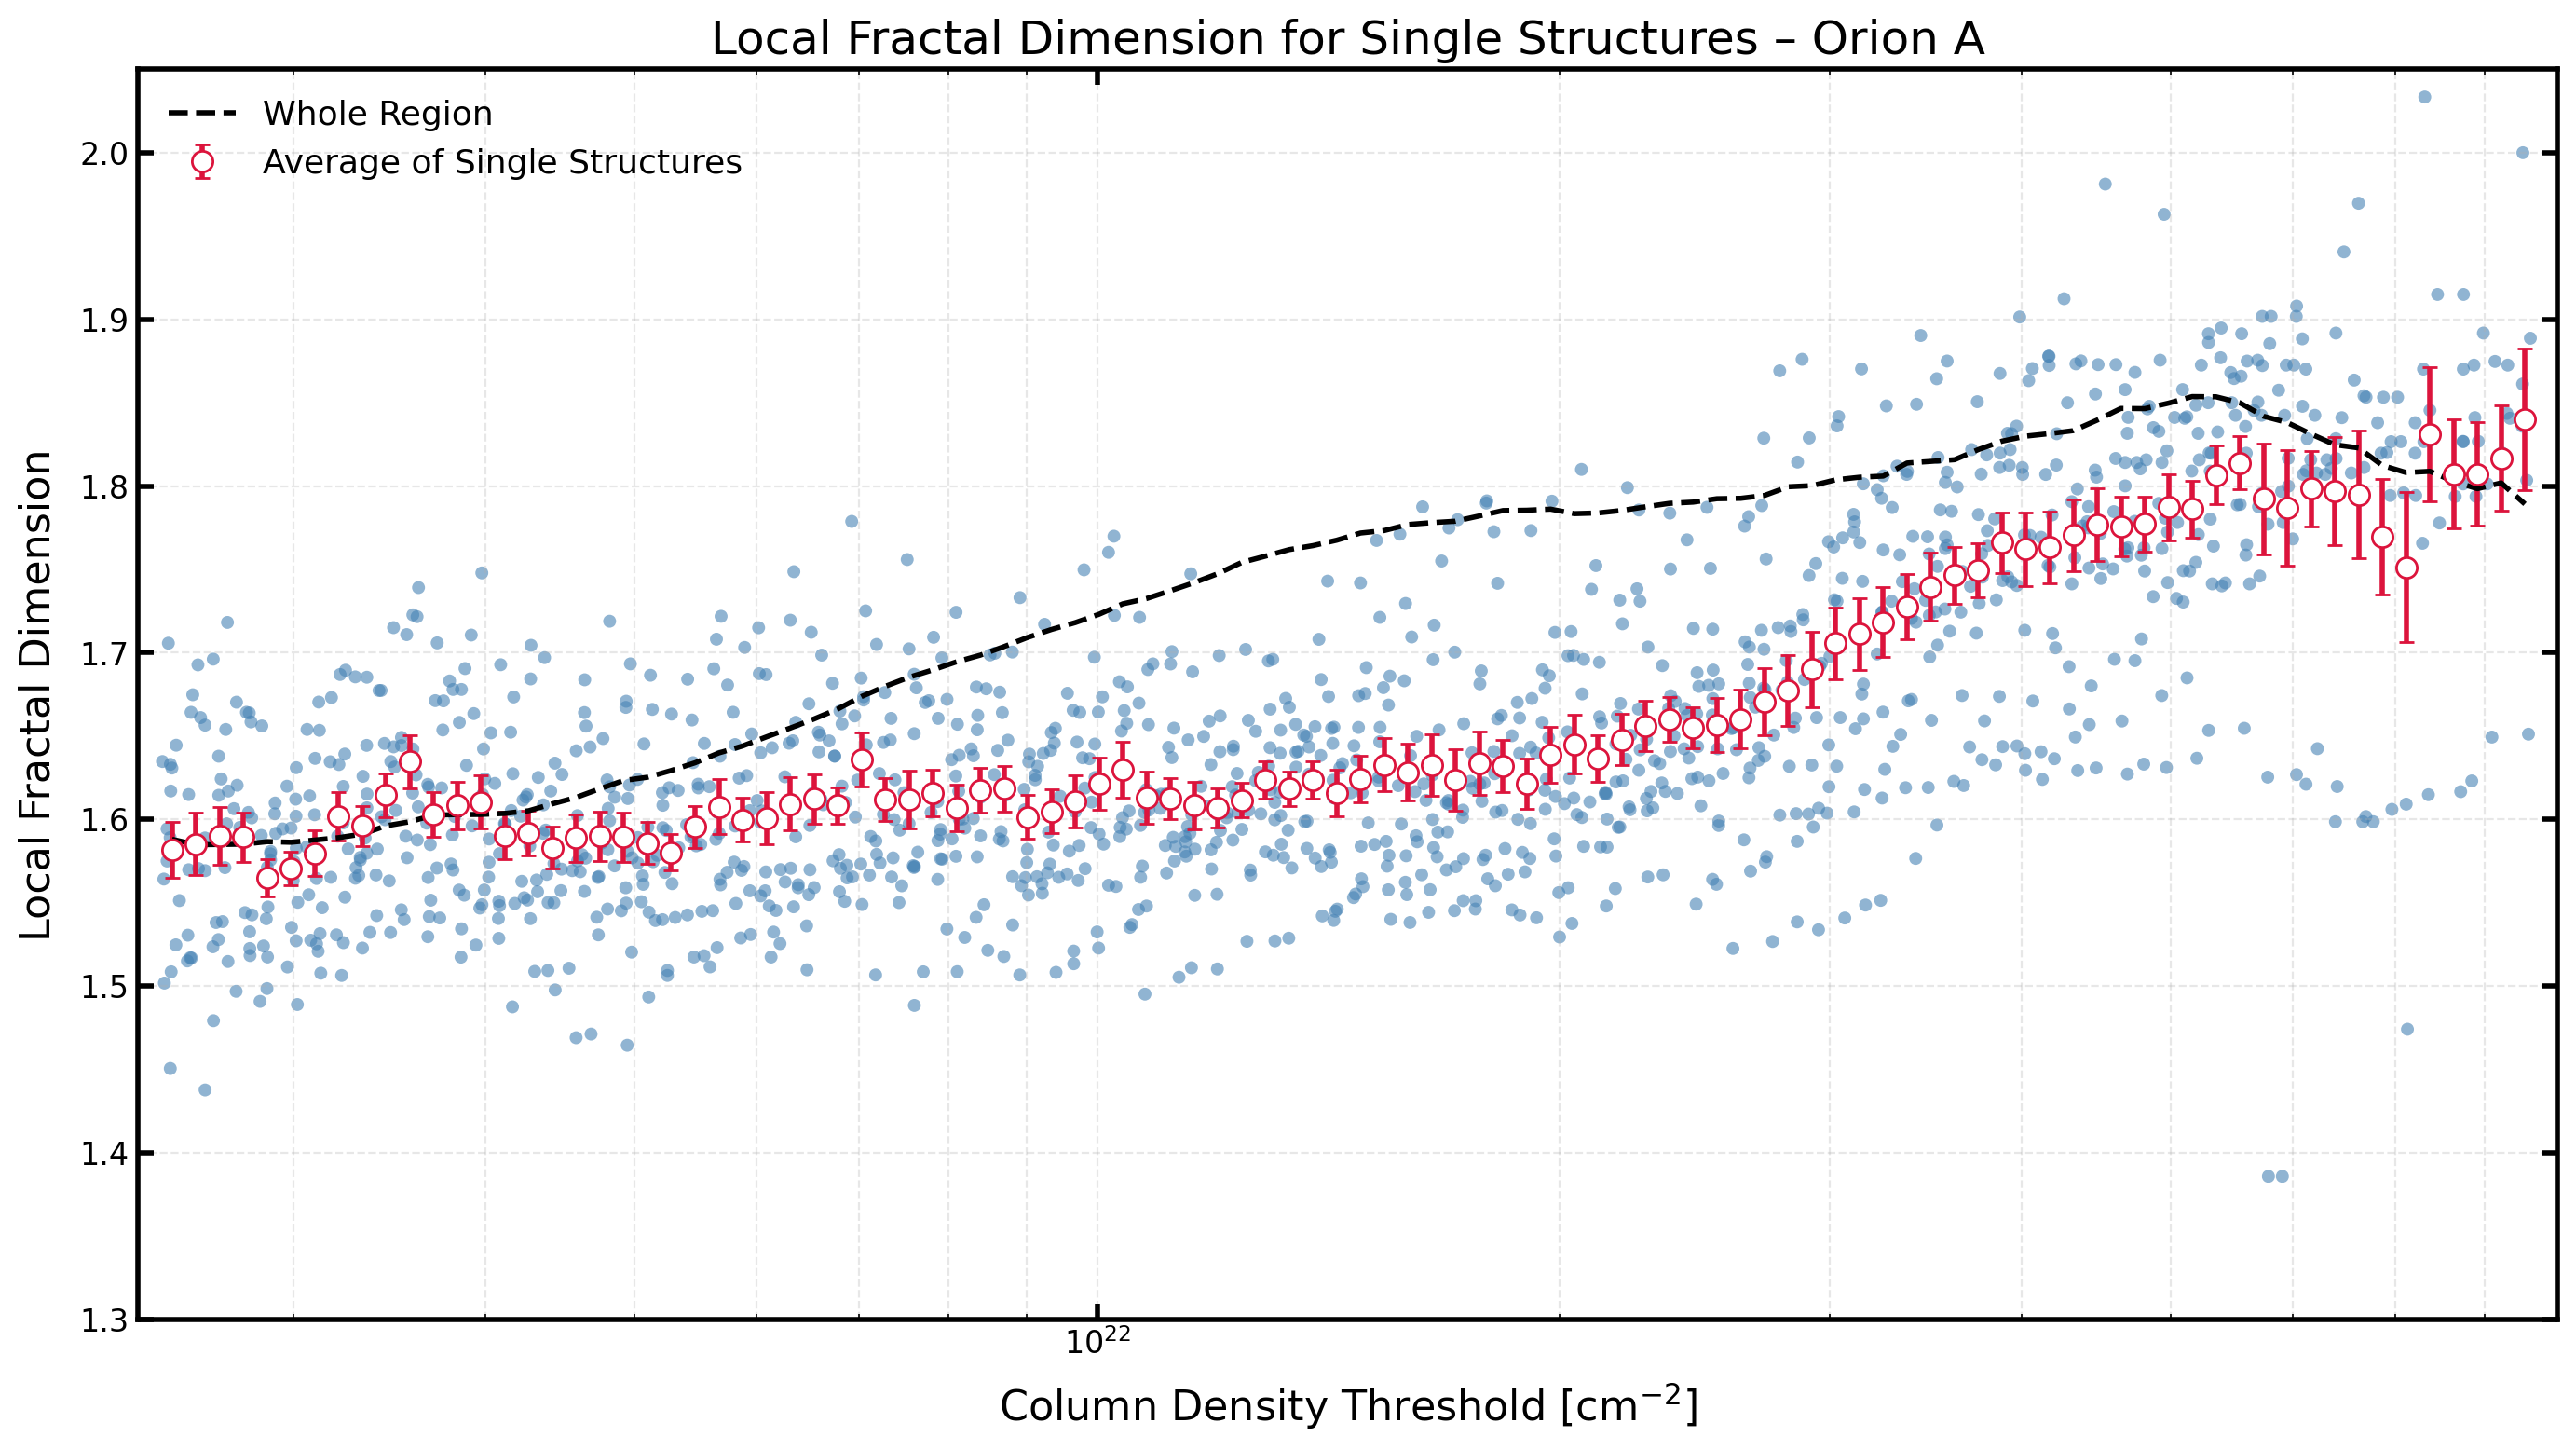
\includegraphics[width=0.75\textwidth]{figures/local_Orion_A_single_structures.png}
    \caption{Local fractal dimension for individual structures in Orion~A as a function of column--density threshold. 
    Shown are the mean values obtained from the largest structures at each threshold (with uncertainties), overlaid with the corresponding values from the undifferentiated calculation.}
    \label{fig:local_A_single_structures}
\end{figure}

\begin{figure}[t]
    \centering
    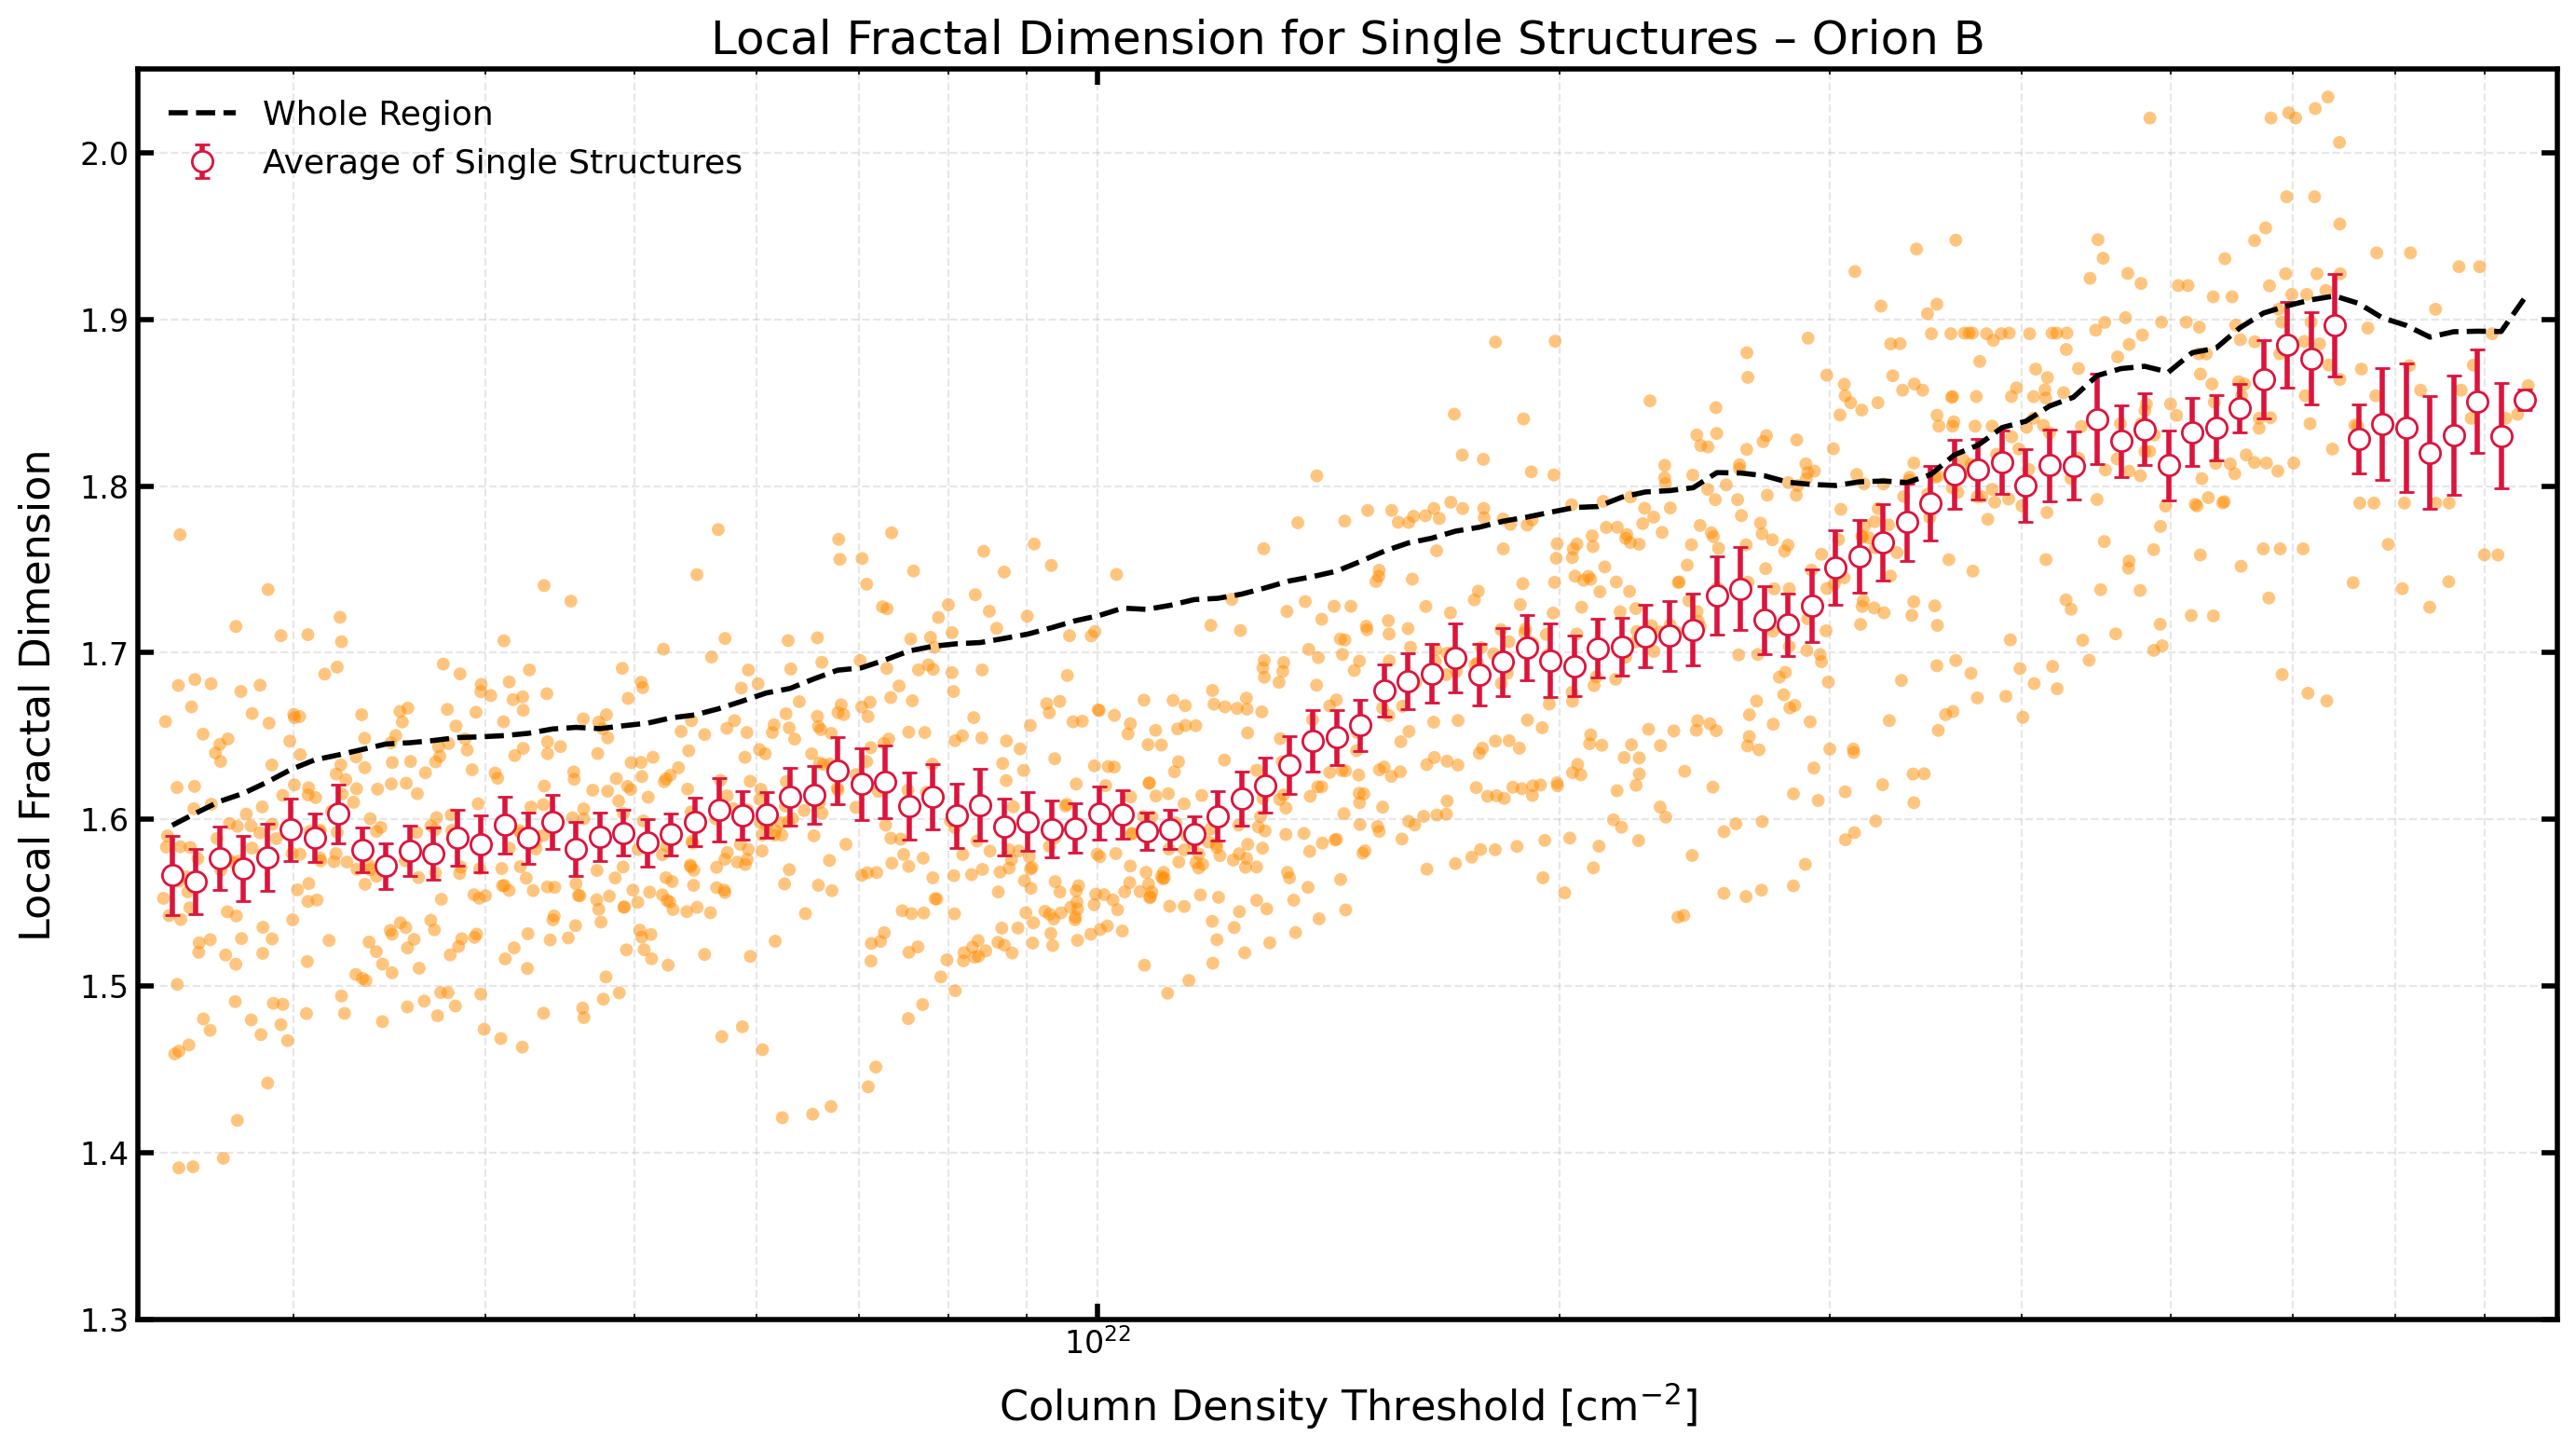
\includegraphics[width=0.75\textwidth]{figures/local_Orion_B_single_structures.png}
    \caption{Local fractal dimension for individual structures in Orion~B as a function of column--density threshold. 
    As in Orion~A, the mean values from the selected structures (with uncertainties) are overlaid with the results from the undifferentiated calculation.}
    \label{fig:local_B_single_structures}
\end{figure}

\subsection{MSD Plane}

To investigate how the fractal properties relate to the physical characteristics of the cloud, we computed the mass, size, and local fractal dimension for each connected structure identified at every column-density threshold in the dendrogram hierarchy.  
These quantities were then plotted against each other, with the local fractal dimension encoded as color.  

The resulting Mass-Size-Fractal Dimension (MSD) planes are shown in Figure \ref{fig:MSD_orion_A} for Orion~A, Figure~\ref{fig:MSD_orion_B} for Orion~B, and Figure~\ref{fig:MSD_orion_A_B} for the combined dataset.  
For reference, the expected scaling relations for idealized filamentary structures (\(A = 10\)) and spherical structures (\(A = 3\)) are overplotted, as done in \cite{Hacar_2025}.

\begin{figure}[t]
    \centering
    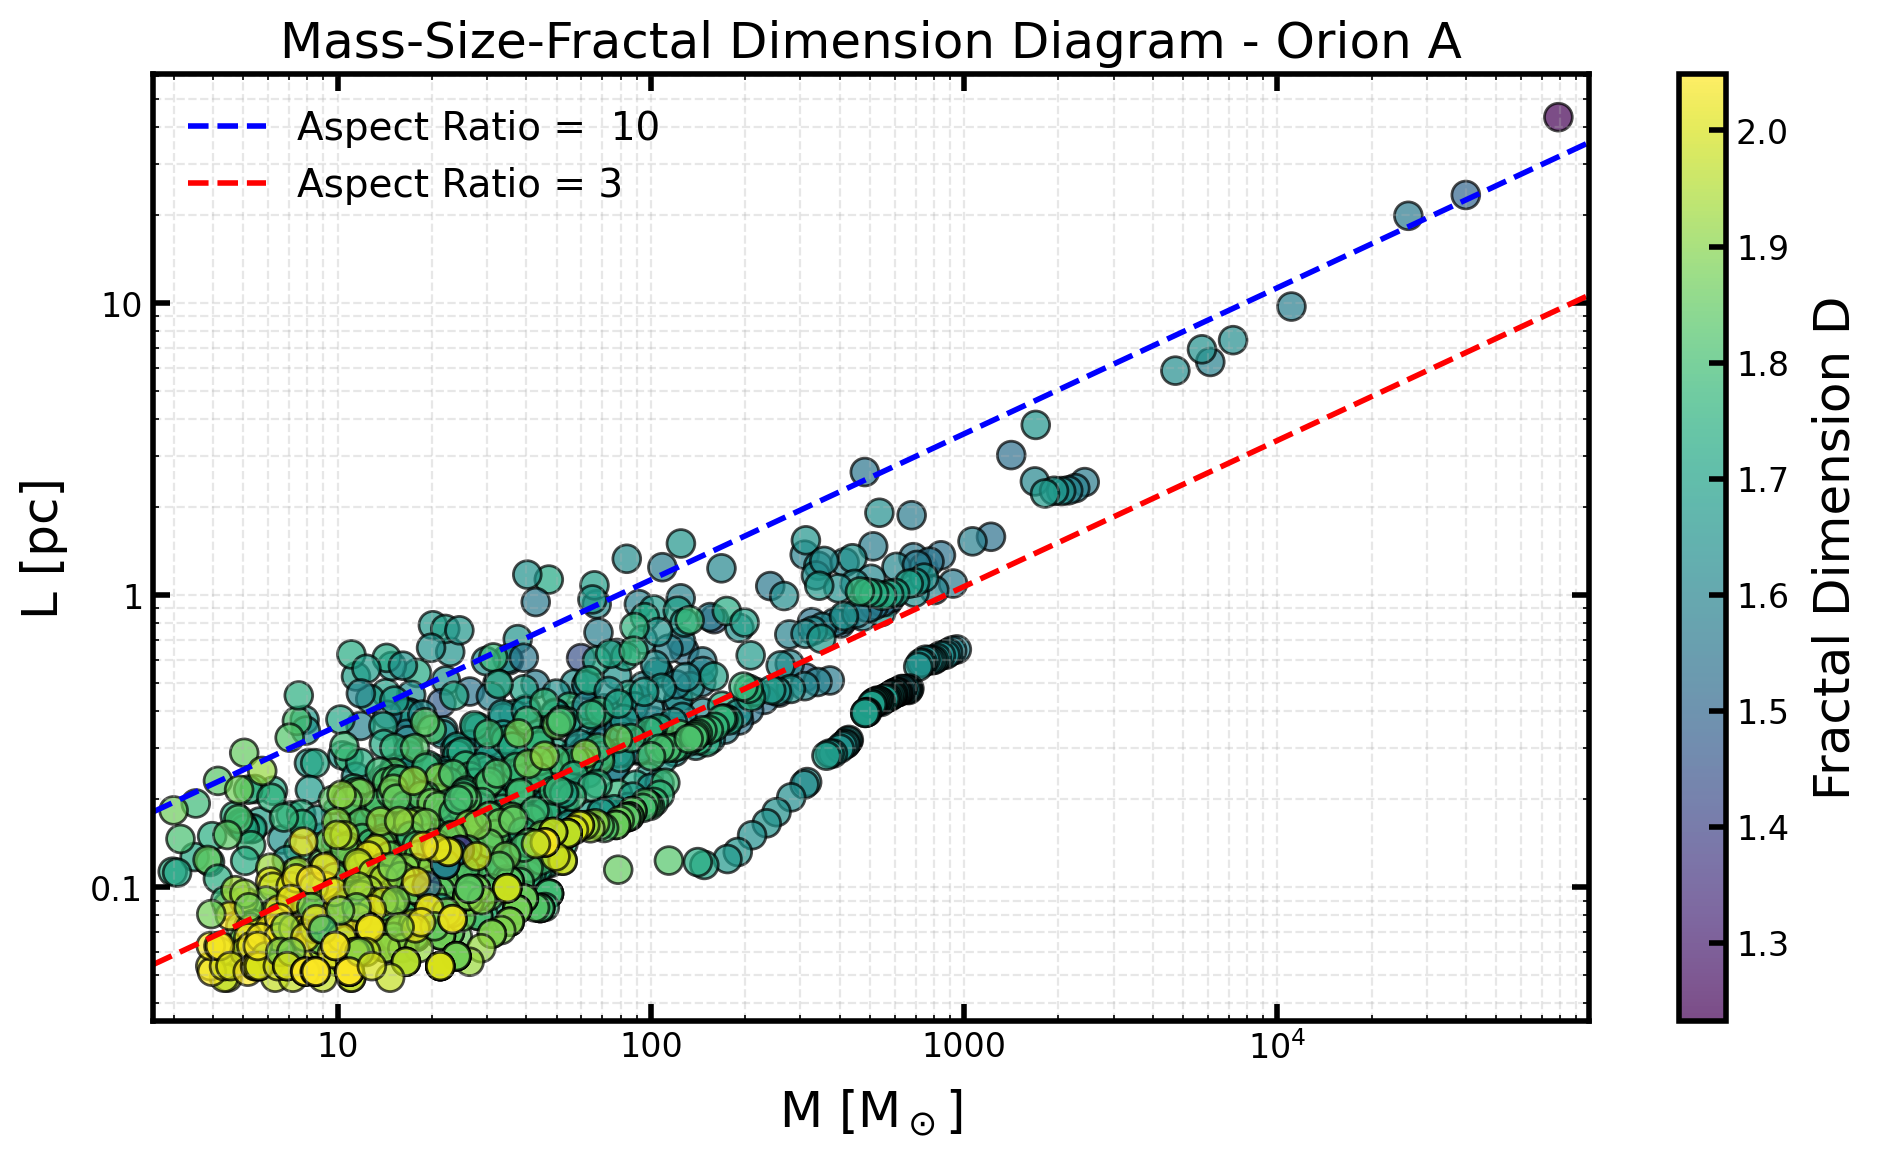
\includegraphics[width=0.6\textwidth]{figures/MSD_Orion_A.png}
    \caption{MSD plane for Orion~A. The color scale indicates the local fractal dimension, and reference scalings for filamentary and spherical geometries are shown as solid lines.}
    \label{fig:MSD_orion_A}
\end{figure}

\begin{figure}[t]
    \centering
    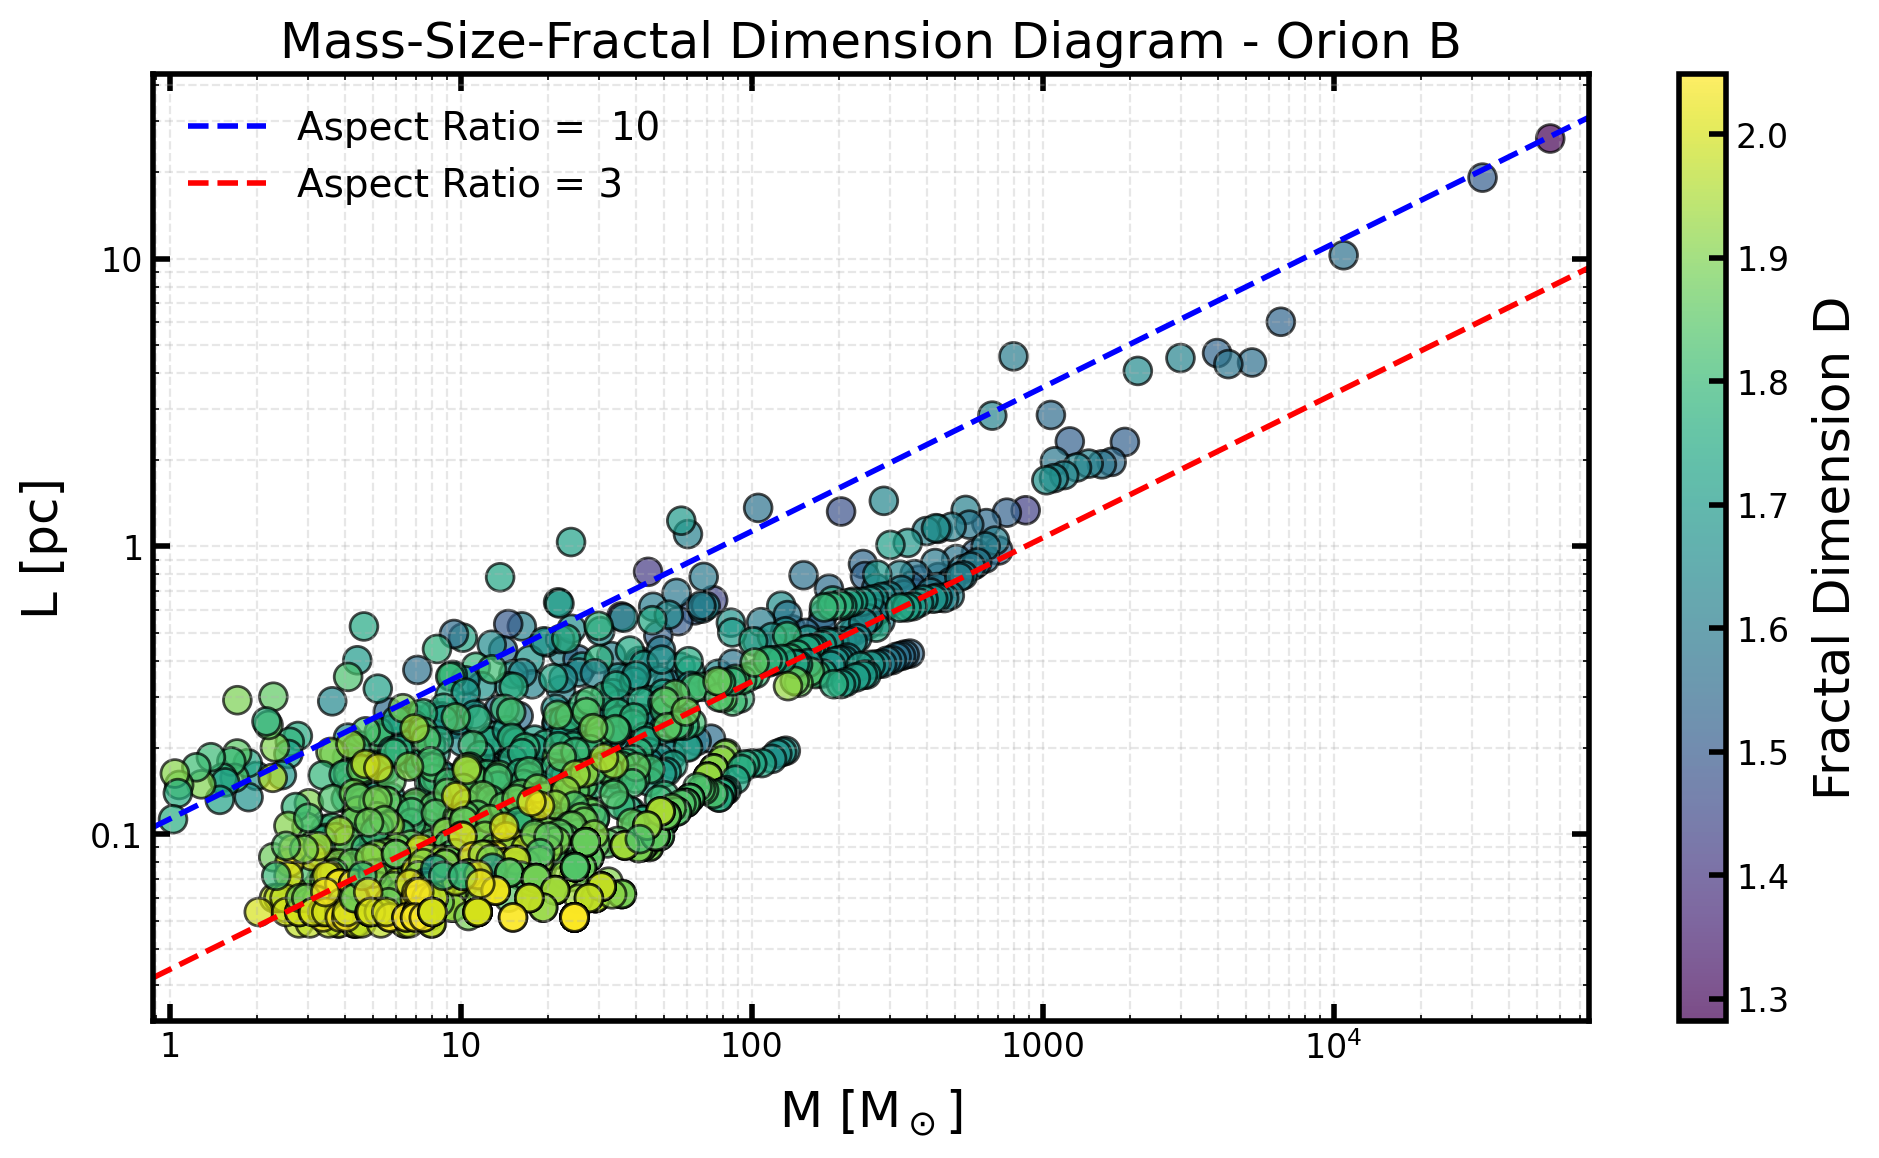
\includegraphics[width=0.6\textwidth]{figures/MSD_Orion_B.png}
    \caption{MSD plane for Orion~B, with color coding and reference scalings.}
    \label{fig:MSD_orion_B}
\end{figure}

\begin{figure}[t]
    \centering
    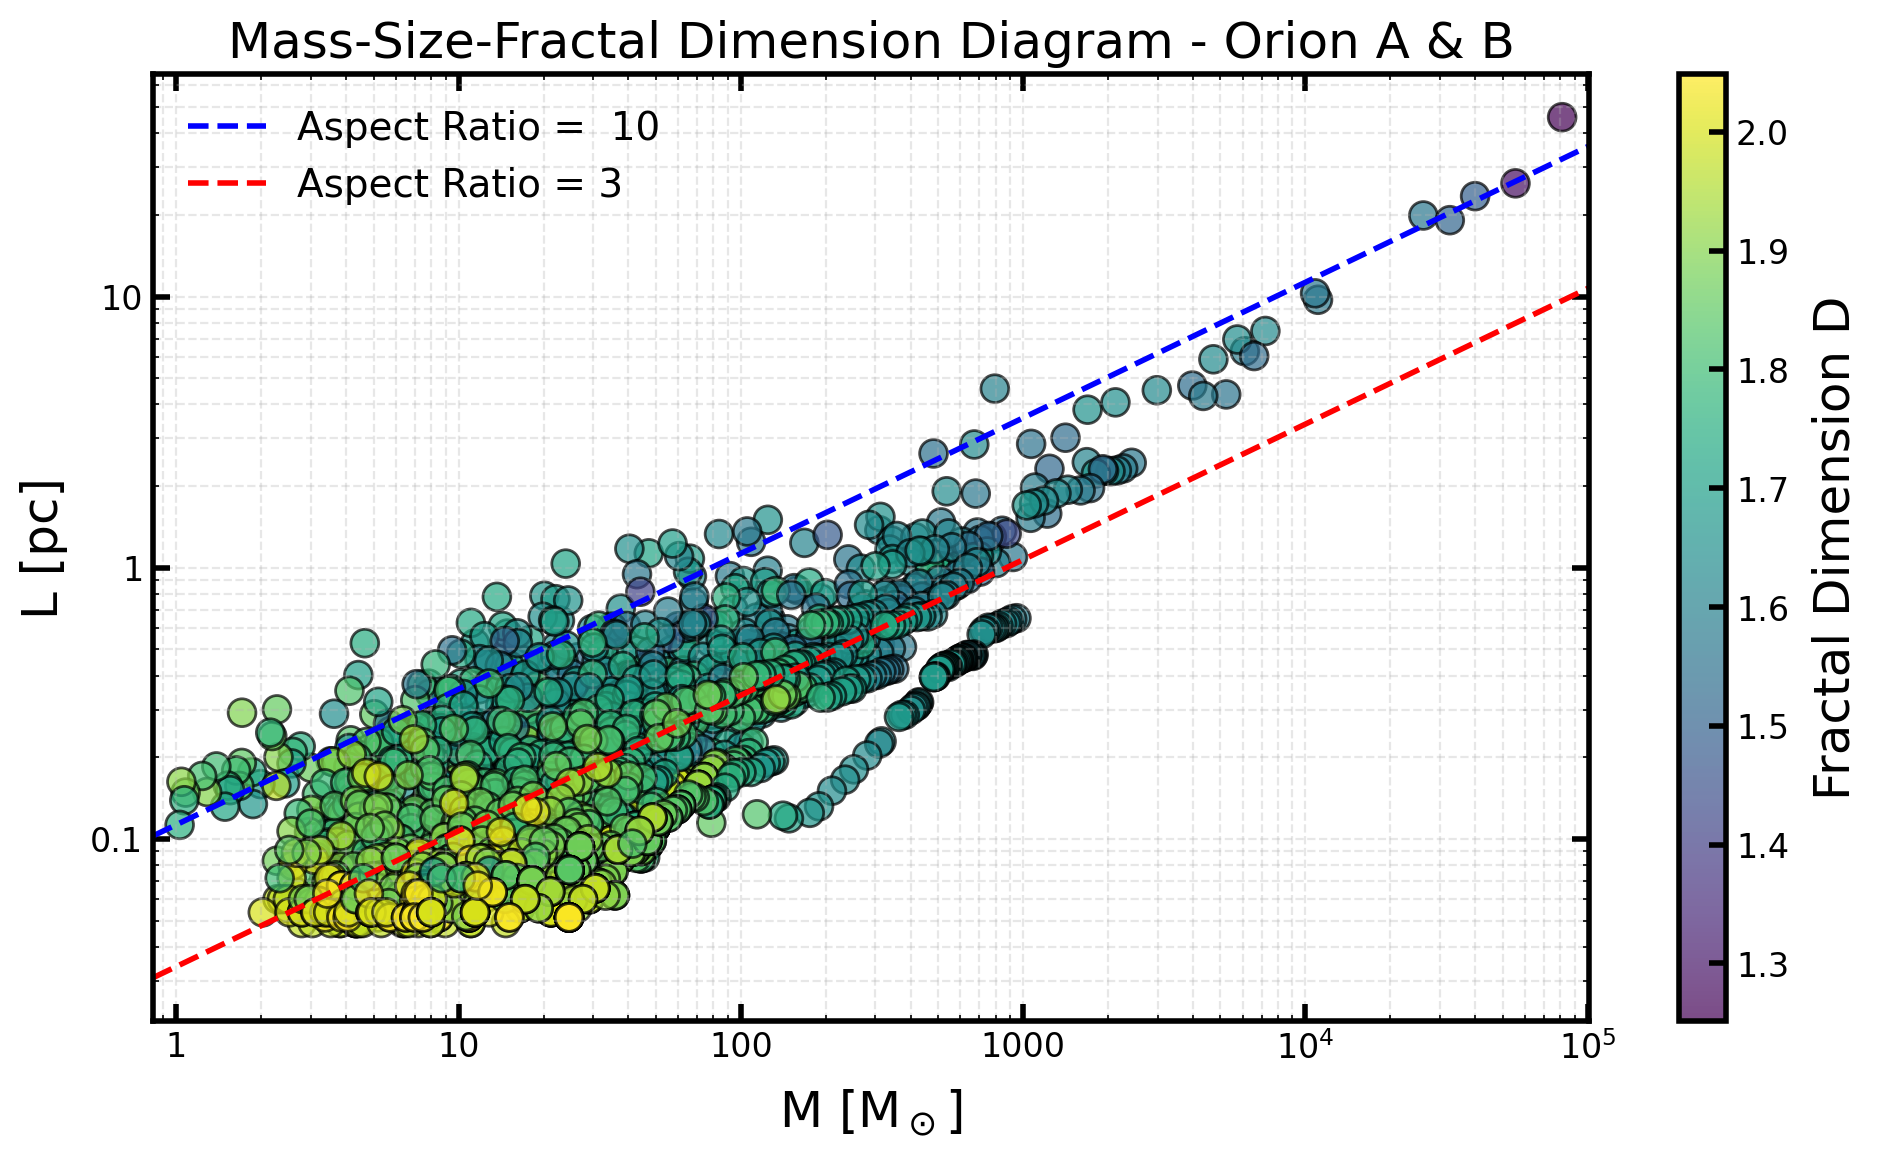
\includegraphics[width=0.6\textwidth]{figures/MSD_Orion_A_B.png}
    \caption{MSD plane for Orion~A and Orion~B combined. The color bar covers the full range of local fractal dimensions across both clouds.}
    \label{fig:MSD_orion_A_B}
\end{figure}

Using this information, we generated spatial maps of the local fractal dimension by assigning to each pixel the value associated with the structure it belongs to.  
If multiple structures overlap, we averaged their values.  
Because of this averaging, the highest values appear slightly reduced compared to the peak values in the previous plots.  
Nevertheless, the maps in Figures~\ref{fig:local_A_map} and~\ref{fig:local_B_map} reinforce the trends already identified in the MSD analysis.

\begin{figure}[t]
    \centering
    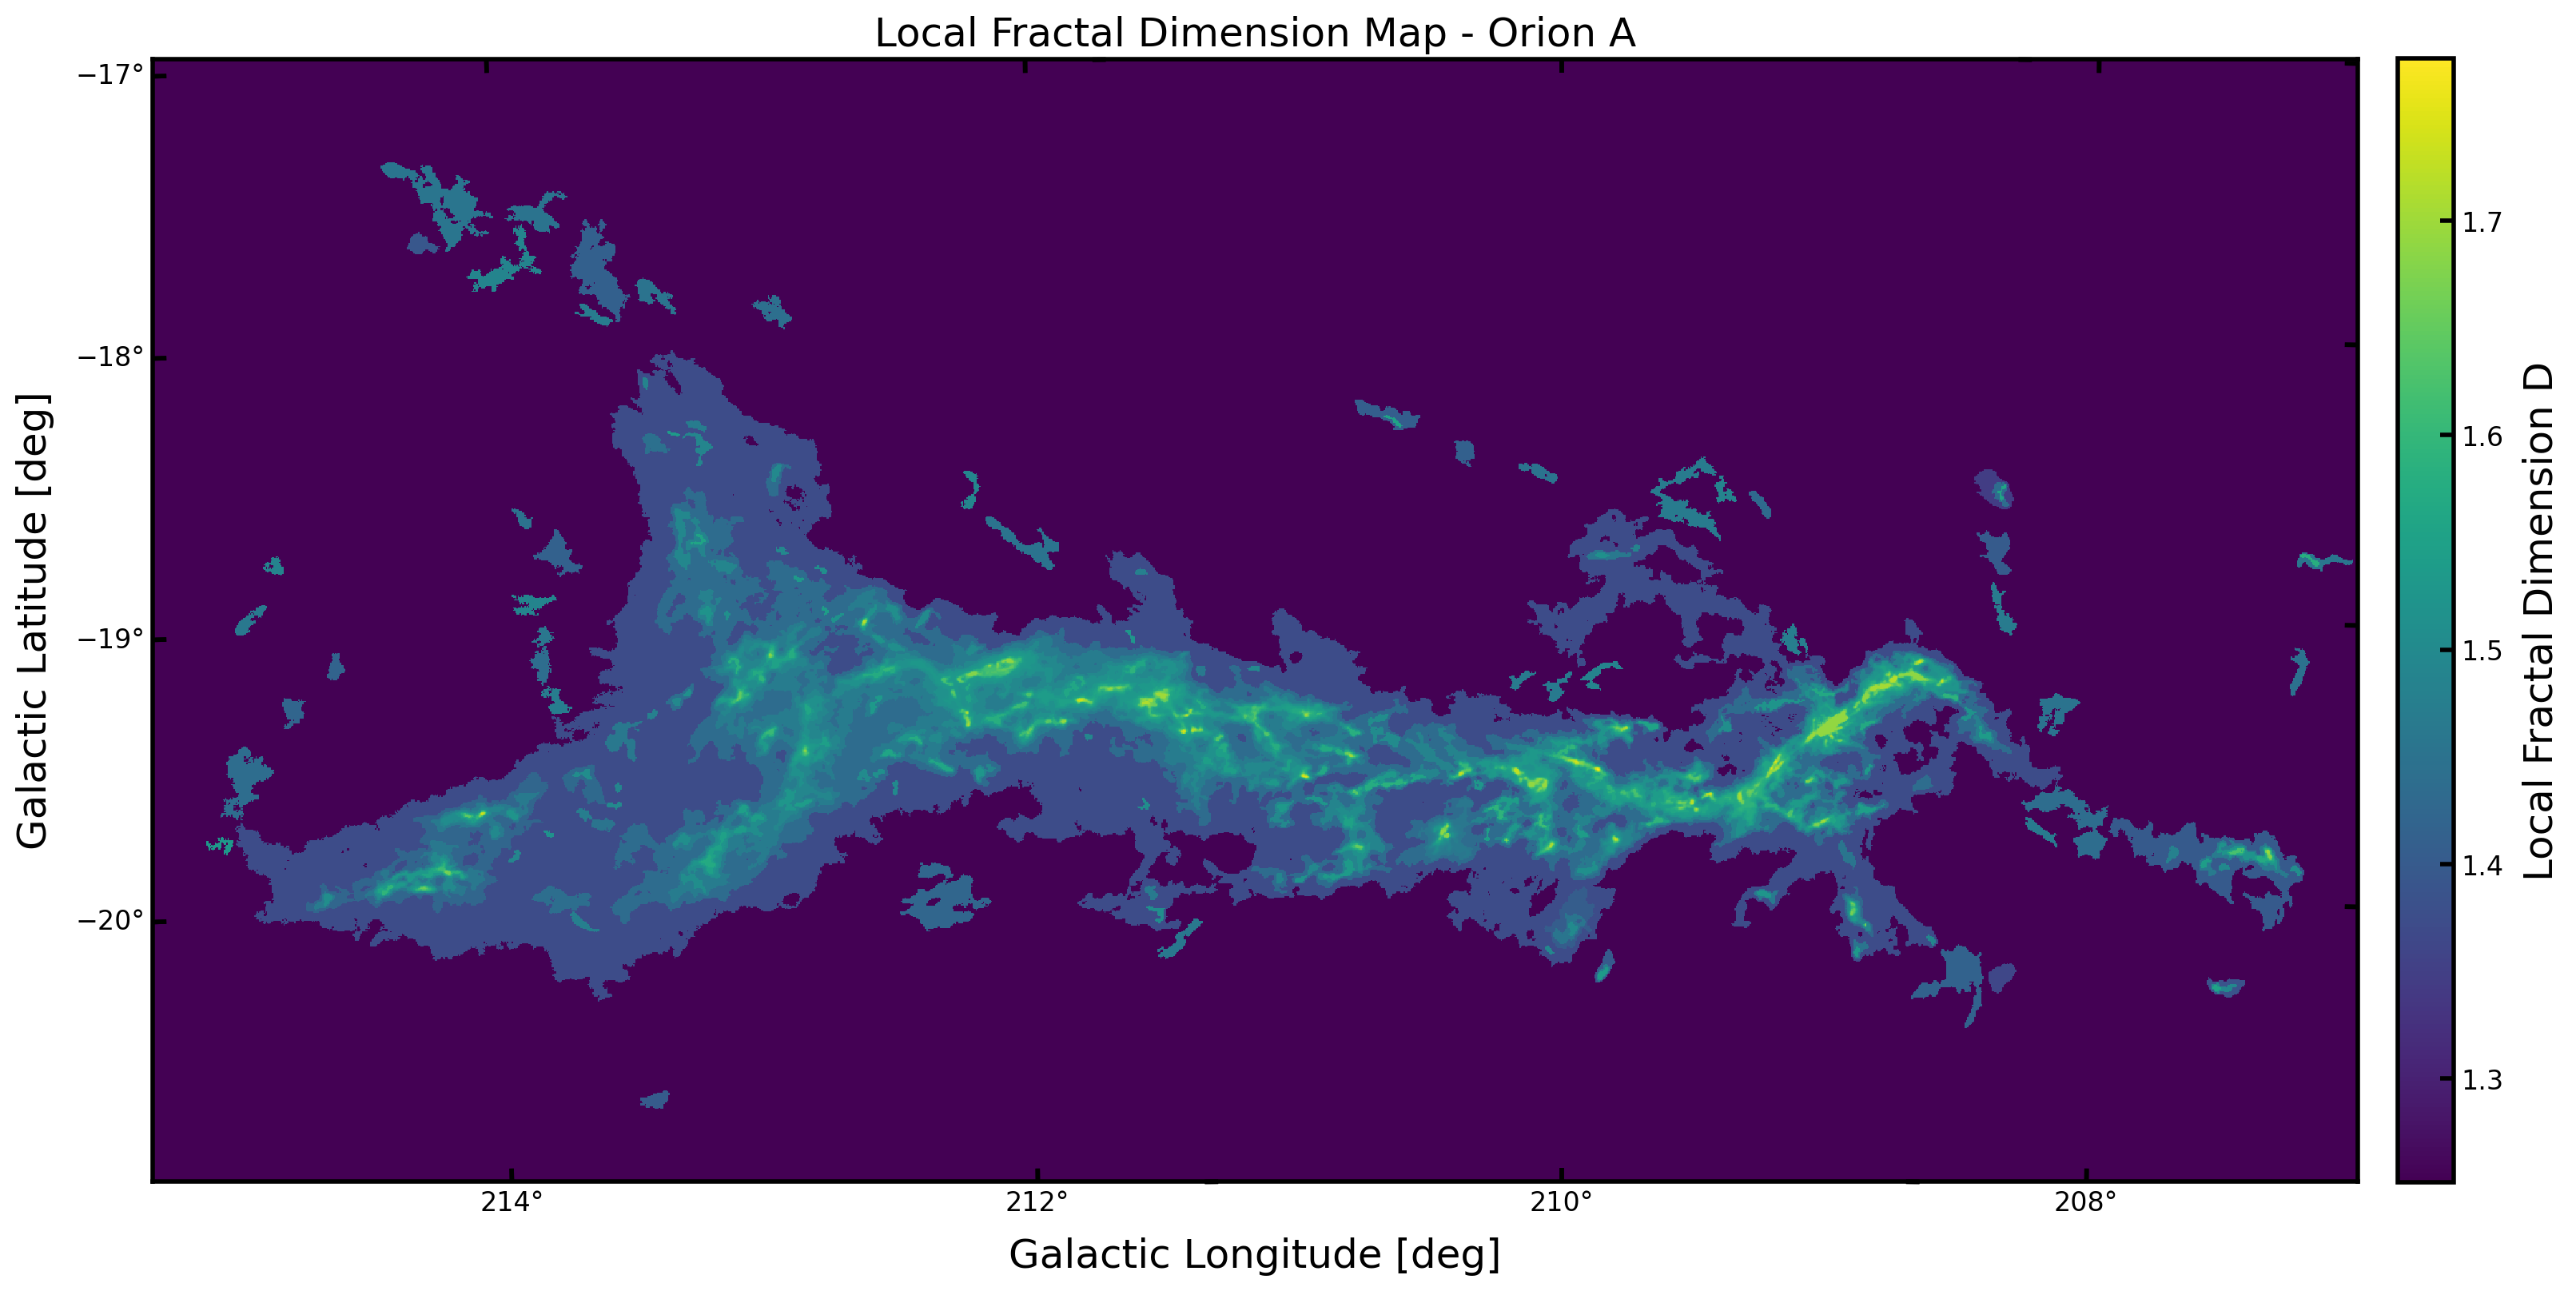
\includegraphics[width=0.75\textwidth]{figures/local_fractal_dimension_map_Orion_A.png}
    \caption{Spatial map of the local fractal dimension for Orion~A. Pixels without assigned structures (NaN) are set to the minimum value of the local fractal dimension.}
    \label{fig:local_A_map}
\end{figure}

% to-do:
% remove the straight lines 
\begin{figure}[t]
    \centering
    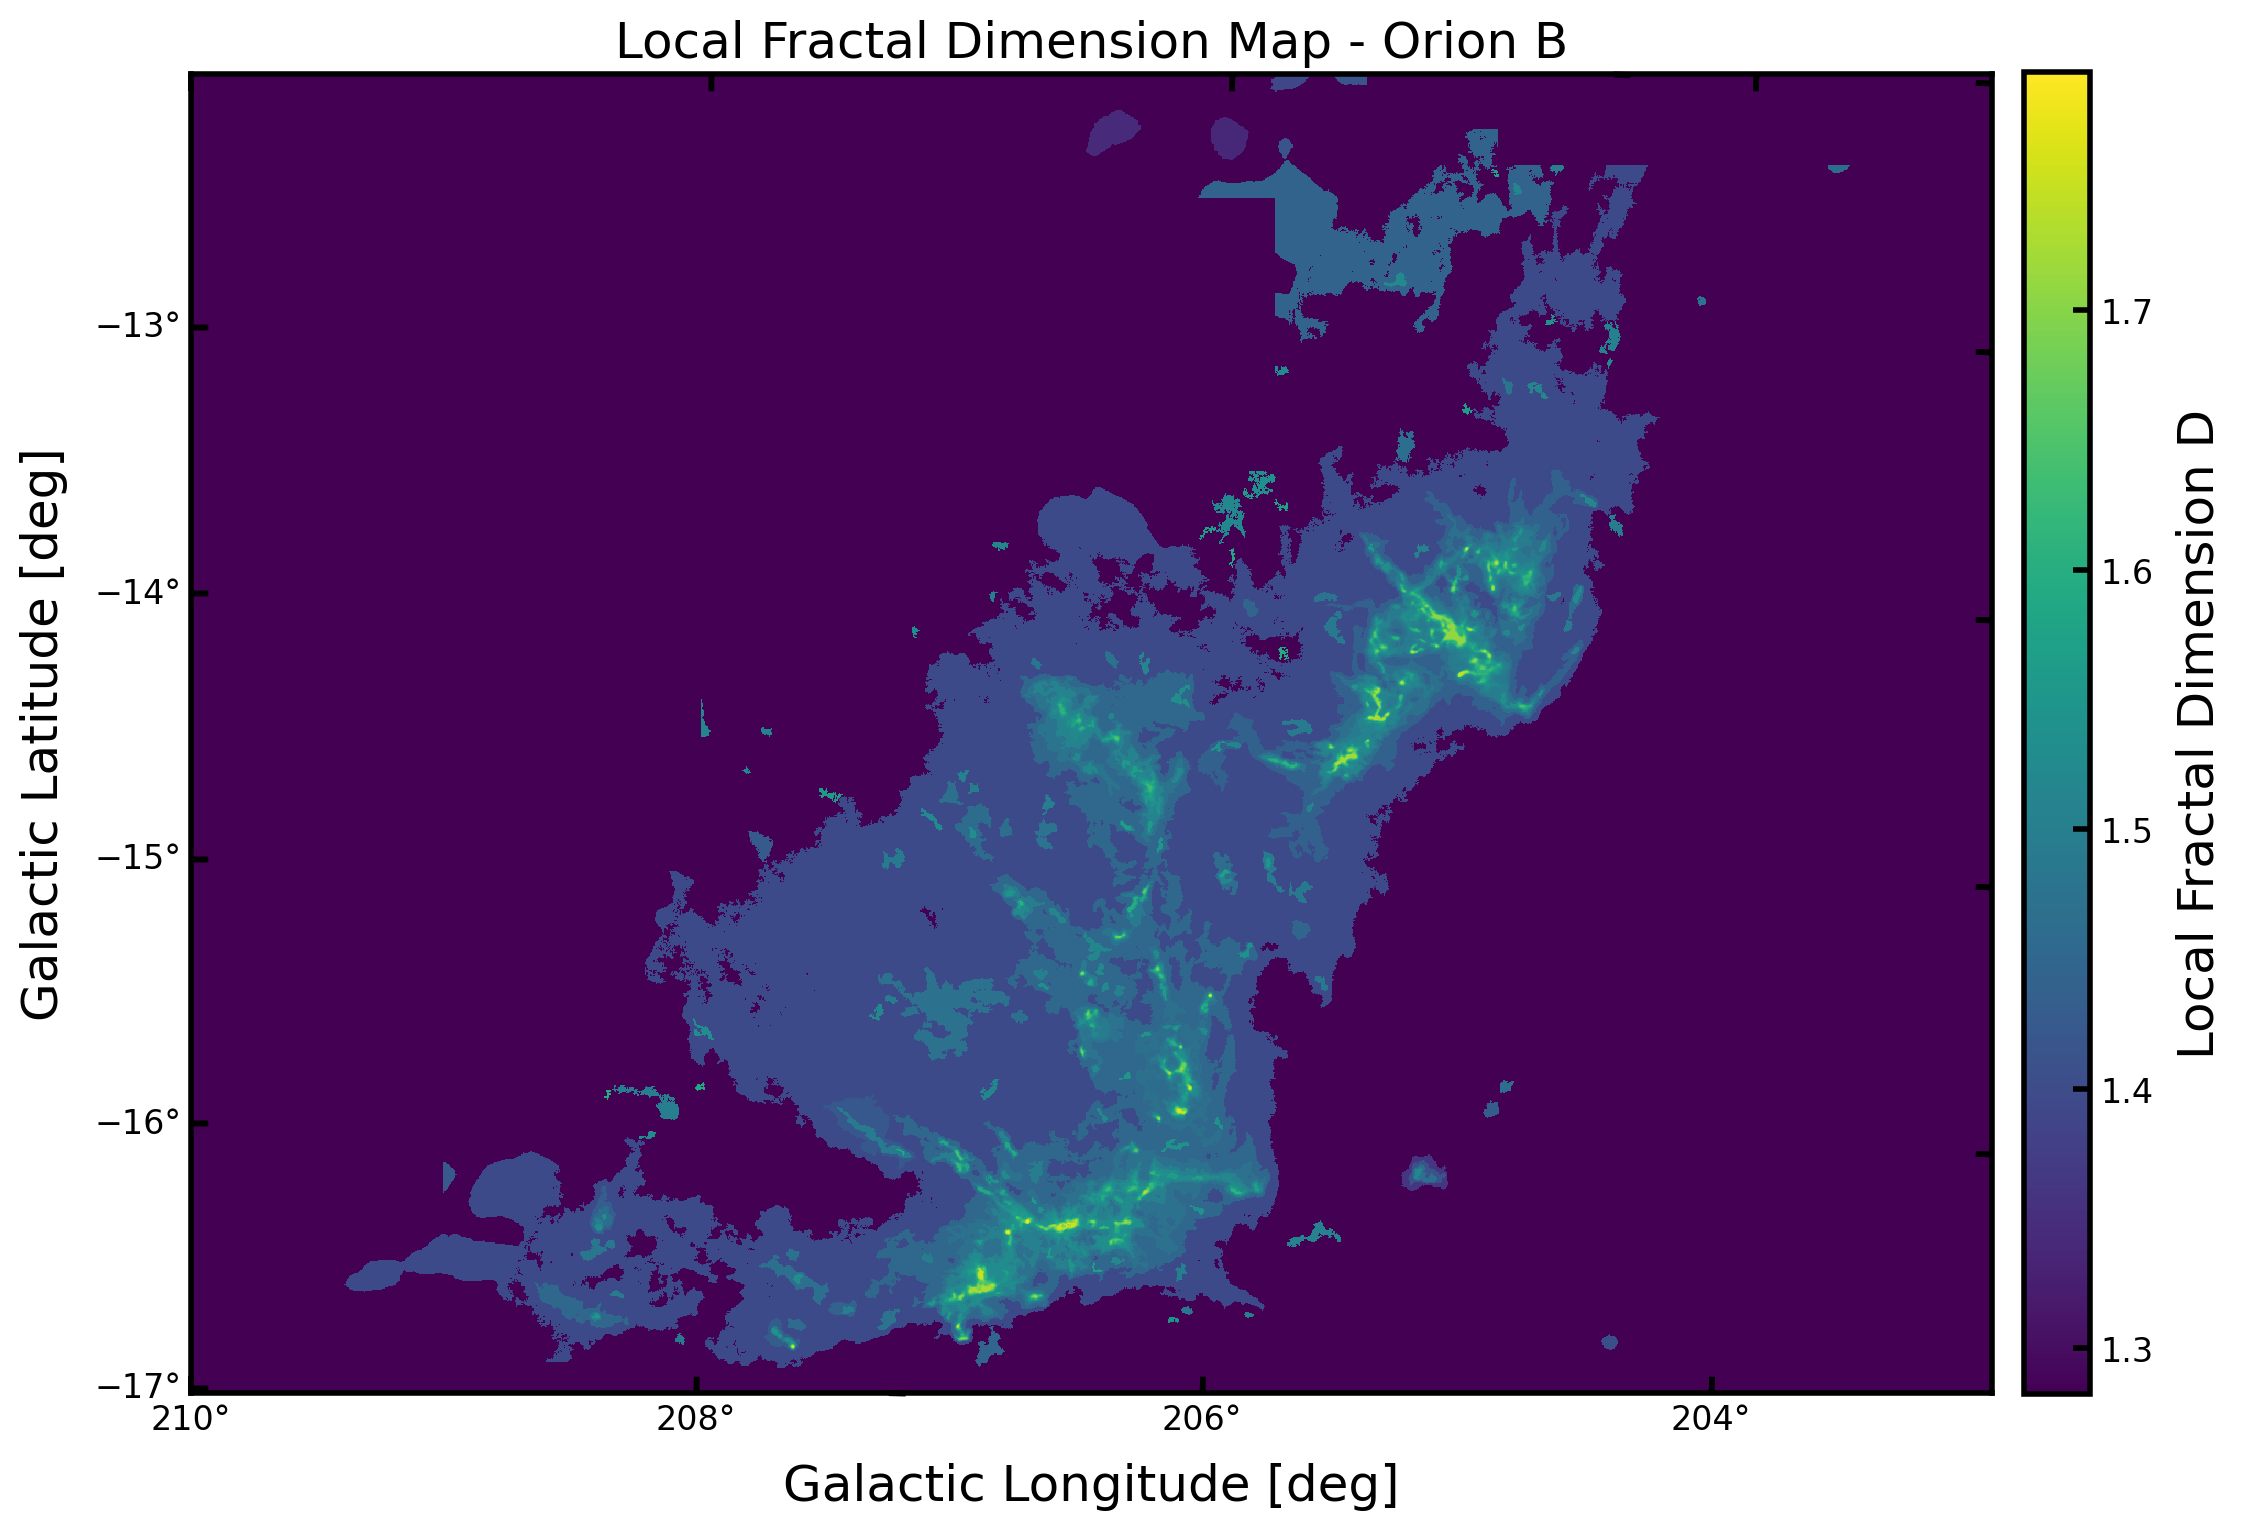
\includegraphics[width=0.6\textwidth]{figures/local_fractal_dimension_map_Orion_B.png}
    \caption{Spatial map of the local fractal dimension for Orion~B. Pixels without assigned structures (NaN) are set to the minimum value of the local fractal dimension.}
    \label{fig:local_B_map}
\end{figure}

An interactive 3D version of the MSD plane is available online at:  
\href{https://simonesped.github.io/MSD_Viz/}{\texttt{MSD 3D Visualizer}}.

Finally, the hierarchical relationships extracted from the dendrogram allow us to track how individual structures break down into substructures.  
This information is visualized in Figures~\ref{fig:MSD_orion_A_lines} and~\ref{fig:MSD_orion_B_lines} in the Appendix, where lines connect each structure to its parent and child structures in the MSD plane.

\section{Connection to Star Formation}

Regions of higher gas density are more conducive to star formation.
To explore this connection, we compared the spatial distribution of the local fractal dimension with the surface density of young stellar objects (YSOs).  
The YSO density maps were obtained by smoothing the distribution of identified YSOs across each region; details of the map construction are provided in the Appendix (Figures \ref{fig:YSOs_density_Map_A}, \ref{fig:YSOs_density_Map_B} for the full sample, Figures \ref{fig:YSOs_density_Map_A_early_stages} and \ref{fig:YSOs_density_Map_B_early_stages}).  
The spatial coverage is naturally limited by the footprint of the available YSO catalog.

We first restricted the analysis to the subset of YSOs classified as early-stage (Class~I and flat-spectrum), which are most likely to be physically associated with ongoing star formation.  
In Orion~A this subset contains 426 objects, while in Orion~B it contains 111.  
Using this subset, the pixel-by-pixel comparison between the YSO density maps and the local fractal dimension yields:
\[
\text{Orion A: Pearson } 0.434, \qquad \text{Spearman } 0.429,
\]
\[
\text{Orion B: Pearson } 0.288, \qquad \text{Spearman } 0.244.
\]

For comparison, we also performed the same analysis using the full YSO sample, without filtering by evolutionary stage.  
The full catalog contains 2818 YSOs in Orion~A and 632 in Orion~B.  
The corresponding correlation coefficients are:
\[
\text{Orion A: Pearson } 0.286, \qquad \text{Spearman } 0.393,
\]
\[
\text{Orion B: Pearson } 0.399, \qquad \text{Spearman } 0.340.
\]

Although the correlations are moderate in both cases, the higher values obtained for the young subset in Orion~A indicate a stronger spatial link between regions of high local fractal dimension and active star formation.  
This supports the interpretation that complex, self-similar structures within the molecular cloud preferentially host the earliest stages of star formation.

% not a lot of pictures here, rather Appendix
\section{Simulations and Uncertainties}

\subsection{Simulations on Global Properties}

\subsubsection{On the Global Fractal Dimension}

To validate the interpretation of the global fractal dimension framework, we performed a series of controlled tests.  
These tests involved applying the fitting routine to mock structures: some were constructed to exhibit a characteristic scale, while others were explicitly scale-free and therefore self-similar.  
As outlined earlier, the method is expected to return a robust and consistent fit only in the absence of a characteristic scale, which would indicate self-similarity.

We first carried out tests on simple geometric figures, in order to confirm the intuition that shapes with simple borders have in this framework a global fractal dimension of 1, and this increase more and more the more complex the boundaries of the shape become. These tests confirmed these expectations.

We then carried out tests on Gaussian Random Fields (GRFs), exploring both GRFs with power-law spectra (scale-free) and GRFs with peaked spectra (dominated by a characteristic scale).  
The simulations consistently confirmed our expectations, showing that the fitting procedure yields more stable and reliable results in the scale-free case, while deviations appear when a characteristic scale is introduced.

We also tested the impact of resolution effects by smoothing the original data with Gaussian kernels of increasing size.  
Even under extreme smoothing, the resulting global fractal dimension varied by no more than -20\,\% relative to the unsmoothed case, indicating that the method is robust within typical observational resolutions. The -20\,\% is also relative to an extreme smoothing case (see Figure \ref{fig:sims_res_global} in the Appendix).

\subsection{Simulations on Local Properties}

\subsubsection{On the Euler Characteristic}

To better understand the expected behavior of the Euler characteristic when applied to real data, we performed dedicated simulations.  
As in the previous tests, the main inputs were Gaussian Random Fields (GRFs), chosen for their well-defined statistical properties and the expectation of a symmetric response.  

The simulations confirmed this expectation: the Euler characteristic exhibits a symmetric profile as a function of the threshold, with a clear maximum in connectivity at the central peak and a gradual decrease on either side.  
This behavior closely resembles a Gaussian bell curve, providing a useful reference pattern for interpreting the results from the actual cloud data.

\subsubsection{On the Local Fractal Dimension}

This section validates the inversion of the perimeter–area (PA) relation and explains how the resulting local fractal dimension should be interpreted in terms of boundary complexity.

We first tested the method on simple, well-understood shapes—straight lines, circles, and Gaussian profiles.  
In these cases it was sometimes necessary to account for the intercept in the original perimeter–area relation (Equation~\ref{eq:perimeter_area}).  
The results were consistent with expectations: lines yielded a dimension of \(D = 2\), simple boxes and circles gave \(D = 1\), and more intricate shapes produced values in between.

We then extended the tests to more complex structures, in particular Gaussian Random Fields (GRFs), to explore how the method behaves in realistic, irregular patterns.  
These experiments revealed a dichotomy that can be described as “sausage vs. hairy caterpillar”:
\begin{itemize}
    \item \textbf{Smooth, compact structures ("sausages")} tend toward \(D(\nu) \approx 2\) in the local PA framework. Their borders are long and coherent with minimal roughness, resulting in a perimeter that scales almost linearly with area.
    \item \textbf{Irregular, space-filling structures ("hairy caterpillars")} tend toward \(D(\nu) \approx 1\). Their boundaries are highly convoluted and expand more slowly with area, leading to a sublinear perimeter–area relationship.
\end{itemize}

A gallery of visual examples illustrating this behavior is provided in the Appendix, and the trends are evident in the observational results (see, for example, Figure~\ref{fig:MSD_orion_A_B}).  
In practice, small and relatively round structures exhibit local fractal dimensions close to 2, whereas larger, more complex structures trend toward 1.

Finally, we examined the effect of resolution on the local fractal dimension using a procedure similar to that employed for the global dimension.  
Smoothing the data with a Gaussian kernel generally reduced the local fractal dimension at most scales.  
At the same time, because the smoothing lowers the highest column-density peaks, the usable column-density range for the analysis becomes narrower.  
This leads to the earlier appearance of artifacts in the PA relation, as documented in the Appendix in Figure \ref{fig:sims_res_local}.

\subsection{Error Estimates}

The uncertainties on the perimeter and area measurements, derived from the simulation procedures described above, are on average approximately 1.6\% for each quantity.  
These uncertainties arise primarily from pixelation effects and the finite resolution of the column–density maps.

An example of the resulting error distributions from a representative simulation is shown in Figure~\ref{fig:uncertainties} in the Appendix.  
The narrow spread around the mean demonstrates that the uncertainty estimates are robust, and that systematic errors remain small compared to the overall dynamic range of the measurements.

\subsection{Comparison with Alternative Methods}

A clear anti-correlation is found when comparing our results with those obtained using the box-counting method, both for the global and the local estimates of the fractal dimension.  
This systematic offset highlights an important scaling dependence: different techniques for quantifying fractal characteristics do not yield directly comparable numerical values.  
Such differences should therefore be carefully considered when interpreting results across studies that adopt different methodological frameworks.

    \chapter{Discussion}

% Start with the big picture.
Our analysis of the Orion A and Orion B molecular clouds reveals a complex interplay between morphology, topology, and star formation activity. 
By combining perimeter–area scaling, Euler characteristic profiles, and mass–size relations, we obtain a consistent picture of how structural complexity varies across column densities and how these variations relate to the presence of young stellar objects.

% Synthesize the fractal dimension results (global and local).
The global fractal dimension is based on the idea that if a structure is self‑similar—i.e., lacks a characteristic scale—its perimeter and area should follow a power‑law scaling, appearing as a straight line in a log–log diagram.  
Turbulence is known to play a key role in organizing structure within molecular clouds, and the perimeter–area method provides a way to quantify how much this self‑similar behavior influences the observed morphology.

Our global perimeter–area analysis reveals distinct structural regimes within Orion~A, with a clear change in slope that reflects different levels of complexity at low and high column densities.  
In contrast, Orion~B maintains a more uniform fractal signature.  
This contrast already begins to suggest that Orion~A and Orion~B are governed by different physical conditions.

For Orion~A, a double fit is required, indicating a change in the underlying physics. The double fit can be seen in Figure \ref{fig:orion_A_global_double_fit}. 
This transition occurs at a column density of \(N = 1.23 \times 10^{22}\,\mathrm{cm}^{-2}\), marking a physically significant scale.  
At this threshold, the structural properties of Orion~A shift, coinciding with the onset of active star formation and the emergence of dense cores \cite{lada2010star}.  
The concurrent changes in fractal dimension and topology at this scale suggest a direct link between the cloud’s morphology and the physical processes driving star formation.

Without applying the double fit, the global fractal dimension is \(D = 1.35 \pm 0.01\). The single fit for Orion A can be seen in Figure \ref{fig:orion_A_global}. 
This value is in good agreement with previously reported fractal dimensions for molecular clouds derived with alternative methods \cite{elmegreen1996fractal}, where typical values are around \(D \sim 1.3\).  
Numerical simulations based on two‑dimensional compressible turbulence in a self‑gravitating ISM also reproduce similar values \cite{1994fns..book..515Y}.  
Note that many studies report the three‑dimensional fractal dimension, which is related to the two‑dimensional value by adding unity.

When the data are separated into two regimes, we obtain \(D = 1.65 \pm 0.01\) at higher column densities and \(D = 0.97 \pm 0.03\) at lower column densities.  
Although a fractal dimension smaller than 1 is not expected in theory, this result is likely influenced by the limited number of data points contributing to the low‑density fit.  
Even so, the trend is informative: a fractal dimension approaching 1 indicates smoother, simpler boundaries, whereas higher column densities exhibit more complex, space‑filling structures.

% to-do: do we see this visually?
With these types of methods, it is important to also consider if our conclusion match what we actually see in the cloud. To this end, we see in the Gallery that: 

Taken together, these results suggest that the processes driving self‑similarity—such as turbulence—become less dominant once dense cores emerge.  
Beyond this threshold, the cloud’s structure deviates from scale‑free behavior, reflecting the impact of star formation on its morphology.

In Orion~B, by contrast, no such break is required.  
This outcome is broadly consistent with expectations, as Orion~B is known to be a more turbulent molecular cloud.  
In such an environment, scale‑free behavior dominates across the column‑density range analyzed, as reflected in the high quality of the single global fractal dimension fit (Figure \ref{fig:orion_B_global}).  
The emergence of cores does not appear to disrupt the hierarchical structuring.  
Together, these findings provide the first elements of a coherent picture described by the Minkowski functionals.

% to-do:do we see this visually?
Again, we need to ask ourselves if visually these conclusions make sense.

It is also instructive to compare these results with measurements obtained for other molecular clouds.  
Studies applying perimeter–area methods or similar techniques have typically found global fractal dimensions in the range \(D \sim 1.2{-}1.4\) for nearby star‑forming regions.  
For example, \cite{falgarone1991hierarchical} reported \(D \approx 1.36\) for CO maps of Perseus and Ophiuchus, while \cite{sanchez2005fractal} found values between 1.25 and 1.35 for a sample of Galactic molecular clouds.  
These values are broadly consistent with the single‑fit results for Orion~A (\(D = 1.35 \pm 0.01\)) and Orion~B (\(D = 1.40 \pm 0.01\)), reinforcing the interpretation that the large‑scale morphology of these clouds is comparable to that of other regions in the Milky Way.

What is less commonly reported, however, is the clear break we observe in Orion~A at \(N = 1.23 \times 10^{22}\,\mathrm{cm}^{-2}\).

Naturally, this method has limitations.  
Numerical errors can arise when calculating perimeters and areas for very small structures at high column densities.  
Straight contours, resulting from limited observational resolution, should also be avoided, as they can distort the scaling relationships on which the method relies.

The local fractal dimension builds on the perimeter–area relation, but in this case the relation is inverted to obtain a proxy for the boundary complexity of individual structures.  
This measure offers a more nuanced view than the global approach, capturing how structural complexity evolves with column density on a local scale.

The local fractal dimension calculated at each column‑density threshold shows a consistent trend toward \(D \approx 2\) at higher thresholds for both Orion~A and Orion~B (Figure \ref{fig:local_Orion_A_B}).  
This behavior appears to arise not from the increasing complexity of individual structures, but rather from the growing, interconnected network of cores, fibers, and filaments that emerge as the cloud fragments at higher column densities.
The average local fractal dimension for both Orion~A and Orion~B is approximately 1.7, which remains within the expected range for molecular clouds. This value suggests that, on average, the boundaries of structures in both regions are moderately complex—more intricate than simple geometric shapes, but not fully space-filling. Such averages are consistent with previous studies and support the interpretation that turbulence and hierarchical fragmentation are key drivers of cloud morphology at these scales.

% to-do: do we see this visually?
% to-do: do the peaks represent something?
Some visual examples are helpful to illustrate this behavior (see Gallery).  
Prominent peaks in the local fractal dimension can be associated to..

Because this approach is less commonly used in studies of molecular clouds, direct observational comparisons in the literature are limited.  
Nevertheless, the trends we identify are consistent with the overall picture painted by the global fractal dimension and align well with our physical understanding of these regions.

The closest analytical work on this topic employs a related framework, the mass–size scaling relation \cite{beattie2019relation}.  
Since mass can be treated as a proxy for area, and size as a proxy for perimeter, this method is conceptually similar to the perimeter–area scaling relation used here.  
In their simulations, they report similar trends in the inferred fractal dimension as a function of Mach number (Figure \ref{fig:beattie_fractal_dimension}).
This comparison demonstrates that the results from our method are supported by independent simulation-based studies and further emphasizes the sensitivity of fractal measures to the turbulent state of the cloud. The uncertainties associated are also similar in magnitude, proving also that our approach is reasonable.

\begin{figure}[t]
    \centering
    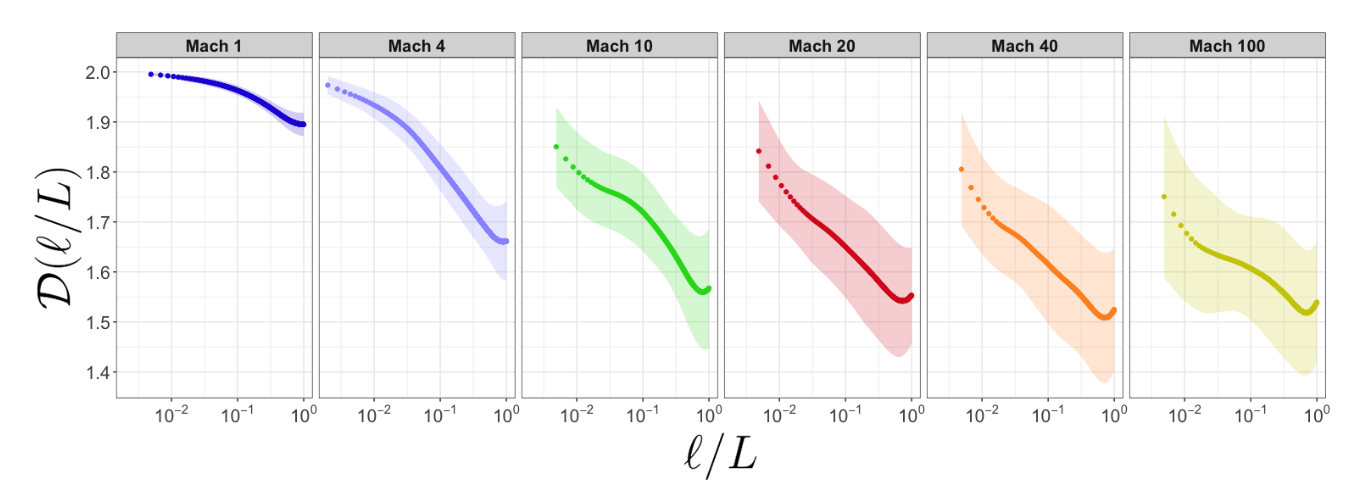
\includegraphics[width=0.8\textwidth]{figures/beattie_fractal_dimension.png}
    \caption{Fractal dimension derived from the mass–size relation as a function of Mach number \cite{beattie2019relation}.  
    Note that the x-axis is inverted relative to the representation used in our plots above.}
    \label{fig:beattie_fractal_dimension}
\end{figure}

As with the global method, certain limitations must be considered.  
Straight edges introduced by limited angular resolution at low column densities, as well as very small structures at the highest column densities, can affect the measurements.  
For these reasons, the usable column‑density range is narrower than the full range provided by the maps.

% Integrate topological insights (Euler characteristic).
Furthermore, the Euler characteristic highlights clear differences between Orion~A and Orion~B.  
Orion~A exhibits a profile that closely resembles the behavior expected from Gaussian Random Field simulations, with a well-defined peak at approximately \(1.64 \times 10^{22}\,\mathrm{cm}^{-2}\).  
This threshold is significant, echoing the transition seen in the global fractal dimension analysis, and marks the emergence of dense cores within the cloud.

In contrast, Orion~B shows no such pronounced peak, instead displaying a more gradual, almost linear decrease.  
If Orion~B is indeed more strongly influenced by turbulence, this behavior is consistent with a more scale-free, less clustered structure, where the appearance of dense cores is more gradual and widely distributed.  
The topological analysis therefore reinforces the notion that turbulence governs the structural evolution of Orion~B, while Orion~A undergoes distinct transitions closely tied to star-formation thresholds.

% explain visually some more also connected to the stuff above
Visual examples of the changes in the Euler characteristic for Orion~A and Orion~B are provided in Figures~\ref{fig:Euler_Orion_A} and~\ref{fig:Euler_Orion_B}.  
These figures illustrate how the degree of connectivity and fragmentation evolves as a function of column density.  

In Orion~A, the sharp peak in the Euler characteristic corresponds to a rapid transition from a regime dominated by isolated structures to one in which these structures merge into a more interconnected network.  
The example cutouts in Figure~\ref{fig:Euler_Orion_A} highlight this process: at low column densities, the cloud consists of many disconnected regions, whereas at higher thresholds these regions coalesce into larger, more complex entities.

In contrast, Figure~\ref{fig:Euler_Orion_B} for Orion~B shows a more gradual evolution.  
Here, the Euler characteristic decreases smoothly, indicating that fragmentation and merging occur over a broader range of column densities.  
The visual examples confirm that Orion~B maintains a predominantly filamentary and interconnected morphology across scales, consistent with its interpretation as a more turbulent, scale‑free environment.

Together, these visualizations reinforce the quantitative findings and provide intuitive insight into how topology and morphology change across different physical regimes in the two clouds.

\begin{figure}[t]
    \centering
    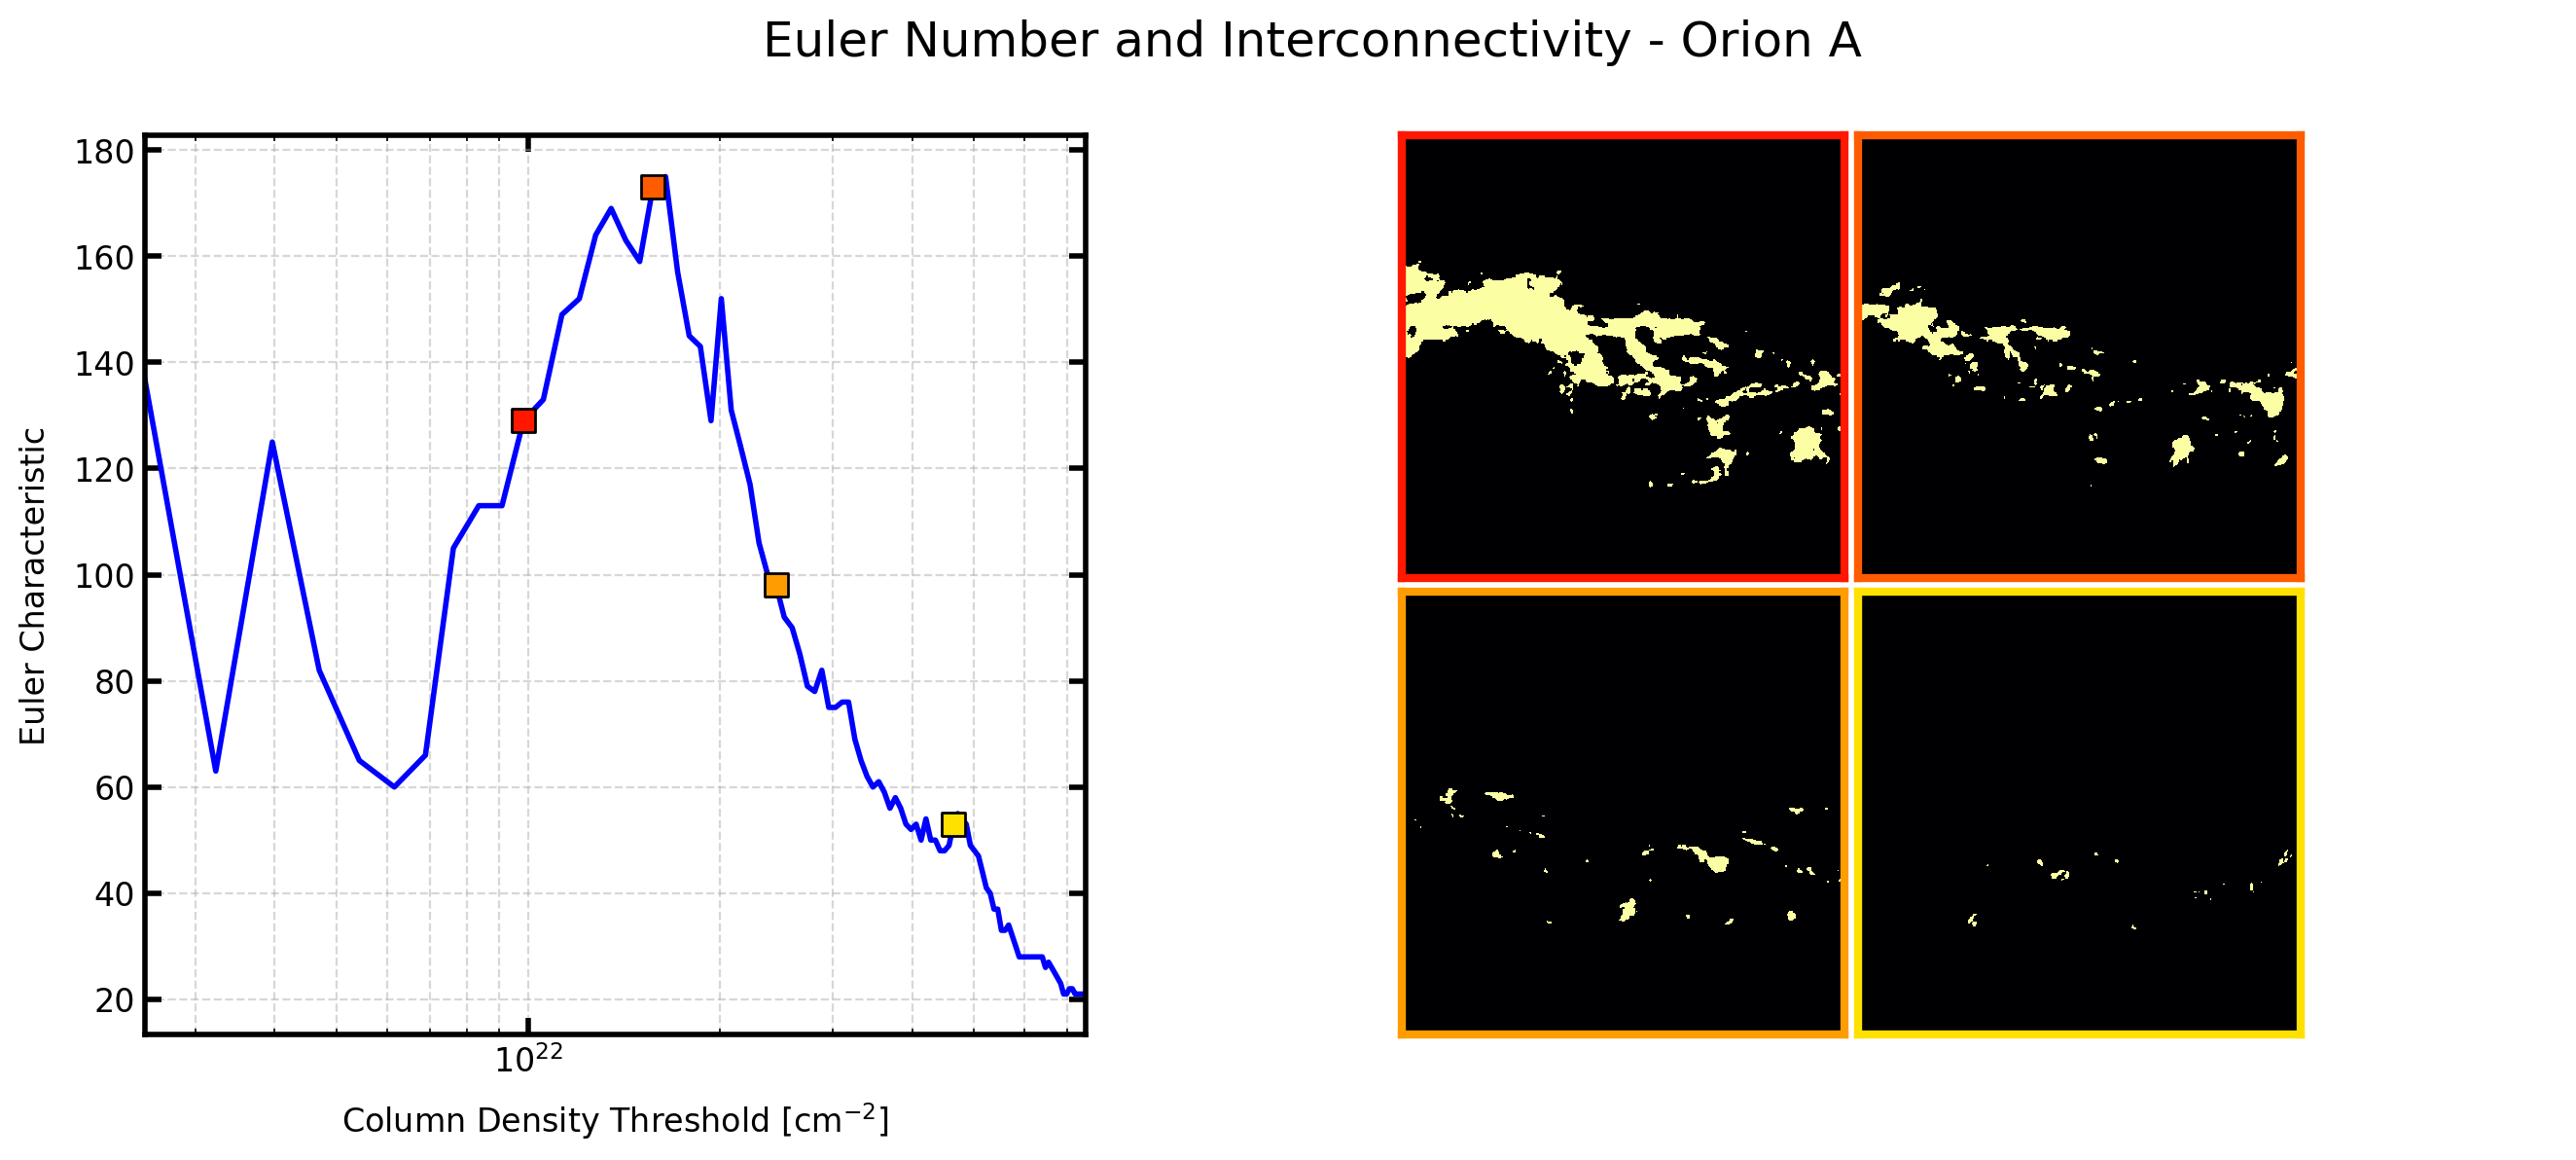
\includegraphics[width=0.8\textwidth]{figures/euler_Orion_A.png}
    \caption{Euler characteristic as a function of column density (left). The right panels show the same zoomed-in area of the cloud at the thresholds indicated by the colored boxes on the graph (Orion A).}
    \label{fig:Euler_Orion_A}
\end{figure}

\begin{figure}[t]
    \centering
    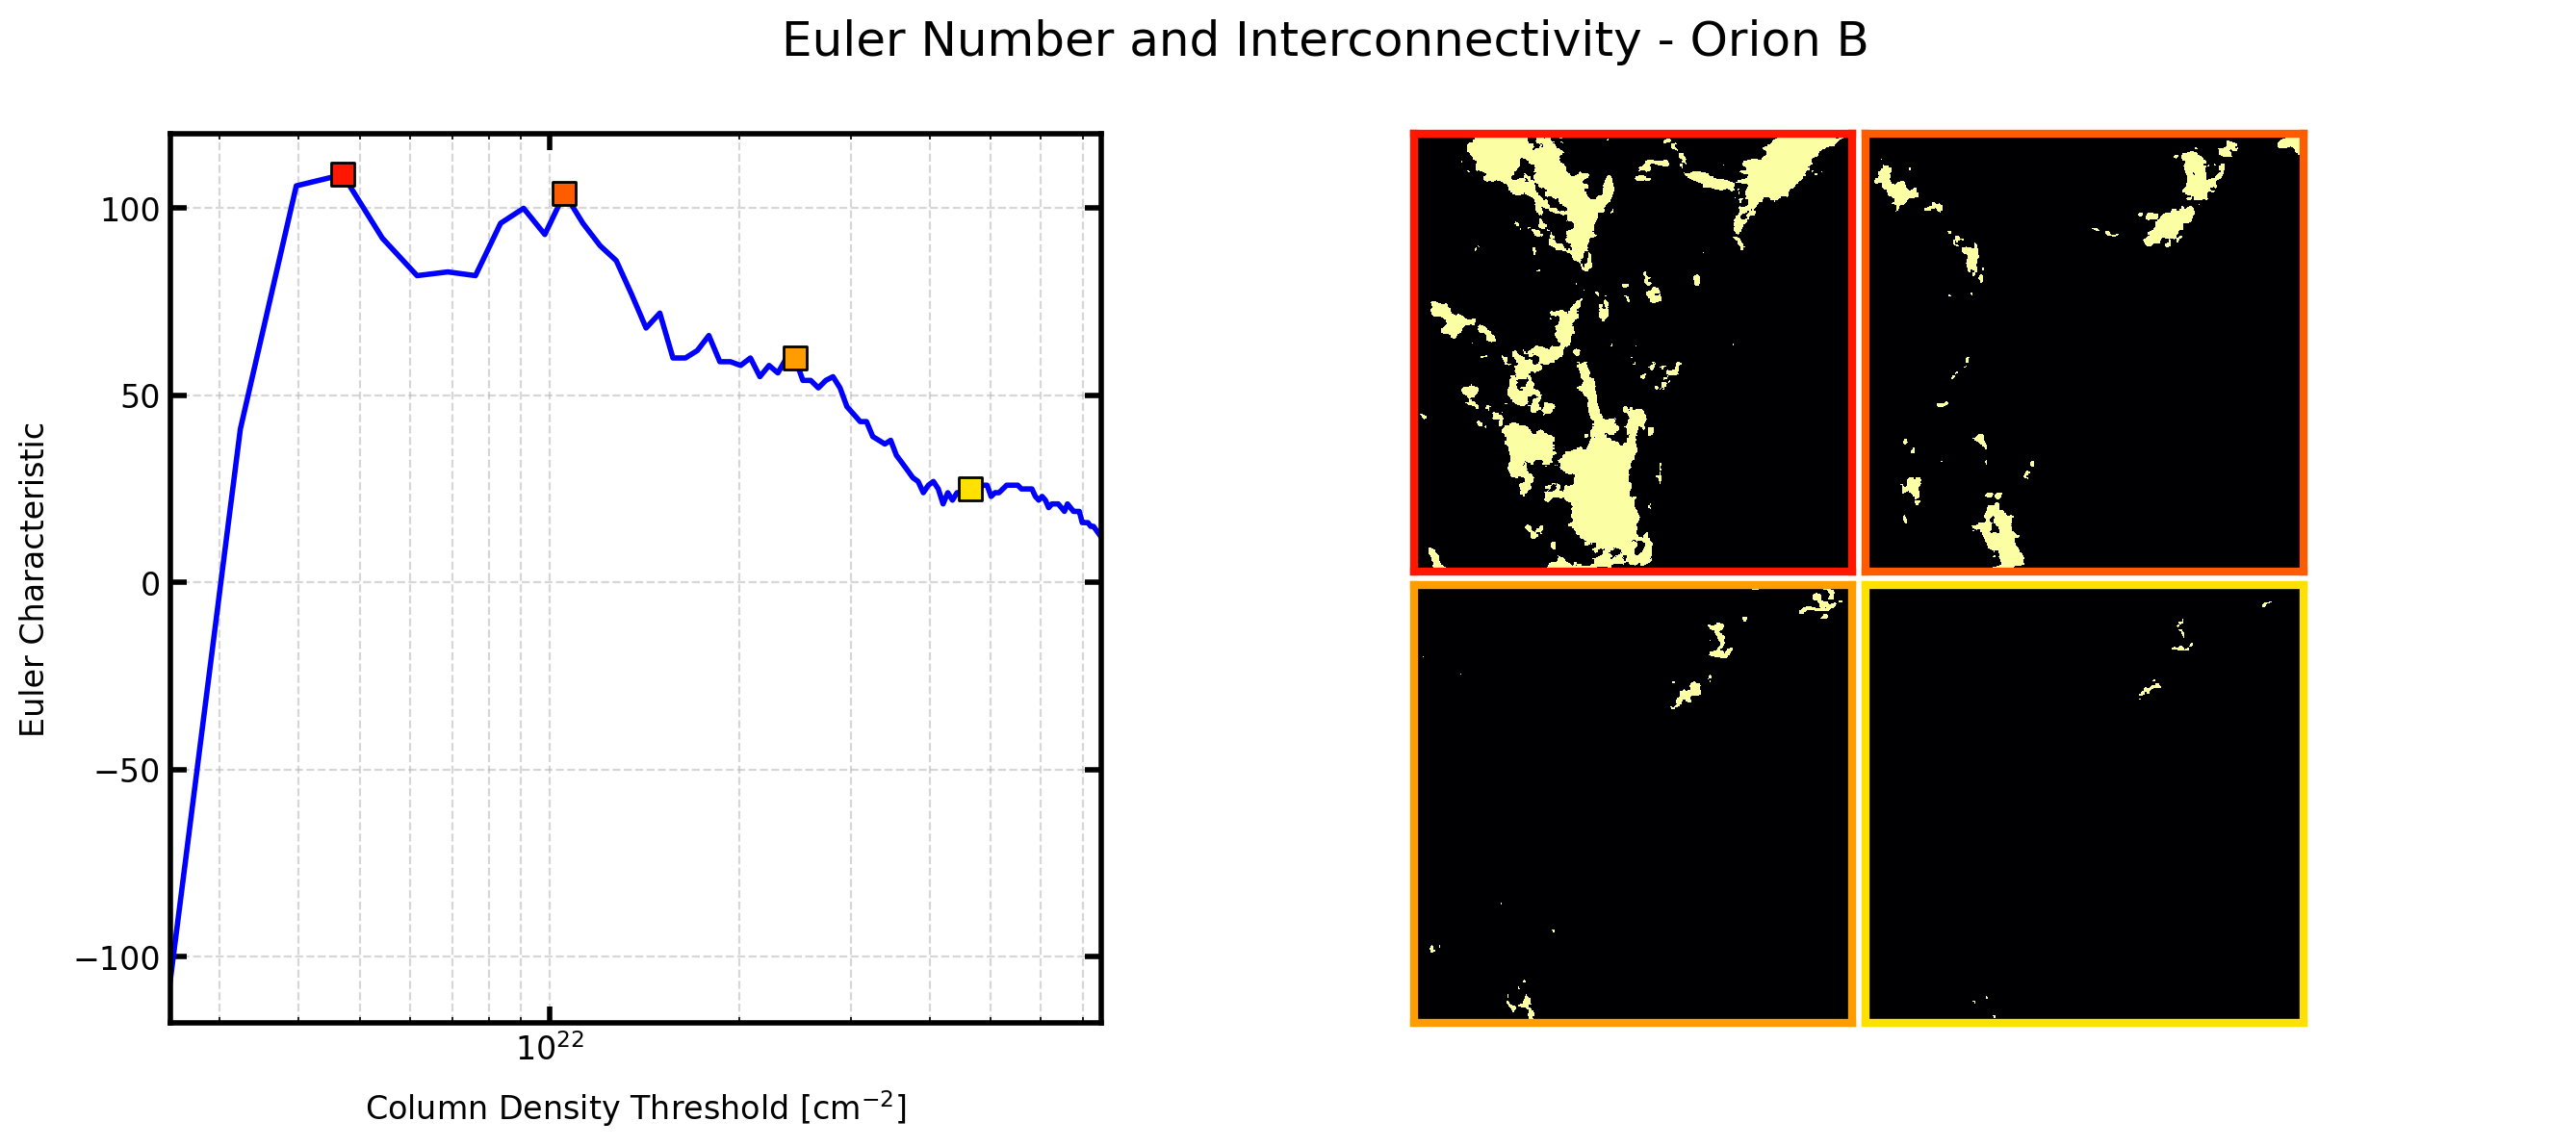
\includegraphics[width=0.8\textwidth]{figures/euler_Orion_B.png}
    \caption{Euler characteristic as a function of column density (left). The right panels show the same zoomed-in area of the cloud at the thresholds indicated by the colored boxes on the graph (Orion B).}
    \label{fig:Euler_Orion_B}
\end{figure}

% Bring in the MSD plane and individual-structure analysis.
The next step in our analysis was to examine individual structures in the context of the local fractal dimension.  
Using the hierarchical segmentation provided by the dendrogram, we tracked the properties and positions of individual components at each column-density threshold.

As an initial step, we analyzed how the local fractal dimension of these structures varies with column density.  
We found that the ensemble of structures broadly follows the trend observed for the entire cloud, but with a shallower dependence and greater scatter (Figures~\ref{fig:local_A_single_structures} and~\ref{fig:local_B_single_structures}).  

These results raise interesting questions.  
While the ensemble as a whole tends toward \(D \approx 2\) (indicating increasing boundary complexity), one might expect that individual structures would appear smoother and simpler at higher column densities, rather than more intricate.  
This apparent tension motivates a closer look at how structure fragmentation and connectivity influence the derived fractal dimension.

Connecting the fractal dimension with mass and size properties further confirmed this puzzling picture: the smaller and lighther (core-like) the structures, the more they tend towards higher local fractal dimension (Figures \ref{fig:MSD_orion_A}, \ref{fig:MSD_orion_B}, \ref{fig:MSD_orion_A_B}).

Visually this can also be confirmed by looking at structures and their fractal dimension here:

% comparison with other methods
In light of these findings, it is instructive to compare our approach with more historically used methods for estimating fractal dimensions in molecular clouds.  
Classical analyses, such as those presented in \cite{elmegreen1996fractal}, often relied on a scale-counting relation of the form
\[
N(\lambda > L) \propto L^{-D},
\]
where \(N\) is the number of self‑similar structures larger than a given scale \(L\), and \(D\) is the inferred fractal dimension.  
While this method provides a useful first‑order characterization of cloud hierarchy, it is inherently limited to counting structures across scales and does not directly incorporate information about their shapes, perimeters, or connectivity.

By contrast, the perimeter–area approach used in this work captures not only the size distribution of structures but also the complexity of their boundaries and how that complexity evolves with column density.  
When combined with topological diagnostics such as the Euler characteristic and hierarchical segmentation via dendrograms, this method offers a more nuanced view of how morphology and topology change across different physical regimes.  
Rather than yielding a single, scale‑averaged fractal dimension, our approach reveals distinct regimes within the same cloud (e.g., Orion~A) and connects those regimes to physically meaningful transitions such as the emergence of dense cores and the onset of star formation.

In summary, while historical methods such as the \( N(\lambda > L) \) scaling have been invaluable in establishing the fractal nature of molecular clouds, the combined perimeter–area and topological analysis employed here provides a more detailed, physically interpretable framework that links structural complexity directly to the underlying star‑forming processes.

% Connect to star formation.
% which of the two is forming more stars?
Finally, we decided to explore a possible connection between local structural complexity and star formation activity. To do this, we used the YSO catalogue from \cite{megeath2012catalogue}, extracting a sample of young stellar objects (YSOs) from which we computed a YSO density map. This density map was then correlated with our previously derived local fractal dimension maps (Figures~\ref{fig:local_A_map} and~\ref{fig:local_B_map}). We first analyzed only early-stage YSOs and then repeated the analysis for the full YSO sample for completeness and comparison.

The correlation results, expressed in terms of both Pearson and Spearman coefficients, revealed distinct trends for the Orion~A and Orion~B clouds. In Orion~A, we found a stronger correlation when using the early-stage YSO sample (Pearson: 0.434, Spearman: 0.429) compared to the full sample (Pearson: 0.286, Spearman: 0.393). In contrast, Orion~B showed the opposite behavior, with a weaker correlation for the early-stage sample (Pearson: 0.288, Spearman: 0.244) and a stronger correlation for the full sample (Pearson: 0.399, Spearman: 0.340).

These results hint at possible environmental differences between the two regions.  
In Orion~A, the stronger correlation for early-stage YSOs suggests that the emergence of complex, fragmented structures is closely tied to the onset of star formation.  
Conversely, the weaker or more distributed trend in Orion~B may reflect a more turbulent, less clustered environment where star formation proceeds in a less organized manner, less dependent on localized structural complexity.  
This interpretation is consistent with long-standing observational evidence: Orion~A hosts a significantly higher density of protostars and young stellar objects, including the Orion Nebula Cluster and the Integral Shaped Filament, and is overall far more active in star formation than Orion~B \cite{megeath2012catalogue}.  
The contrasting correlations therefore align naturally with the known difference in star-forming activity between the two regions.

It is important to note, however, that the method is currently limited by the relatively small number of YSOs in the early-stage catalogue and the restricted spatial coverage of the YSO density maps. These limitations make it difficult to draw firm conclusions. Nevertheless, if future studies with larger and more complete datasets confirm these patterns, they would provide valuable evidence for fundamental differences in the star formation environments of Orion~A and Orion~B, and demonstrate the potential of fractal and topological analyses to shed light on the physical conditions governing star formation in molecular clouds.

% End with a synthesis.
Taken together, our analysis provides a cohesive view of the structural and physical differences between Orion~A and Orion~B.  
The combination of global and local fractal dimension measurements, topological diagnostics through the Euler characteristic, and the hierarchical insights from the MSD analysis reveals that both clouds exhibit scale‑dependent behavior, but in distinct ways.  
Orion~A shows clear structural transitions—evident in the change of slope in the global perimeter–area relation and the sharp features in the Euler characteristic—marking the emergence of dense cores and a close connection between increasing morphological complexity and active star formation.  
In contrast, Orion~B maintains a more uniform, filamentary character and exhibits weaker correlations with local complexity, consistent with a more turbulent, scale‑free environment where star formation proceeds in a more distributed manner.  

These findings reinforce the idea that turbulence and self‑similarity dominate cloud structure on large scales, but that localized physical processes such as core formation can imprint strong deviations from scale‑free behavior.  
By integrating fractal analysis with topological measures and comparisons to simulations, this study demonstrates how a multi‑faceted approach can link the morphology of molecular clouds directly to their star‑forming activity, offering a richer and more physically grounded picture than classical methods alone.
    \chapter{Conclusion}

Summary Intensions

Summary Methods

Summary Results and Discussion

outlook! (very important) 

Improvements
-> better/other estimates for uncertainties
-> less limited methods for the connection to star formation through YSO density
-> extend the method to more structures
-> extend testing to more cases?
    
	%add your sources in the bib file and change the style here
    \bibliographystyle{alpha}
	\bibliography{bibliography}
	
	\printglossary[type=\acronymtype]
    \printglossary

    \cleardoublepage{}
	\pagebreak
	
	%add your end matter here
	\appendix{}

	\chapter{Appendix}

This first appendix contains extra graphs and results that mainly compliment the results section. 
\section{Fractal Dimension}
% Dendrograms (maybe)

This section shows more plots regarding the local fractal dimension and the evolution of structures on the Mass-Size-Fractal Dimension graph.
% to-do
% likely to redo, very messy
\begin{figure}[h]
    \centering
    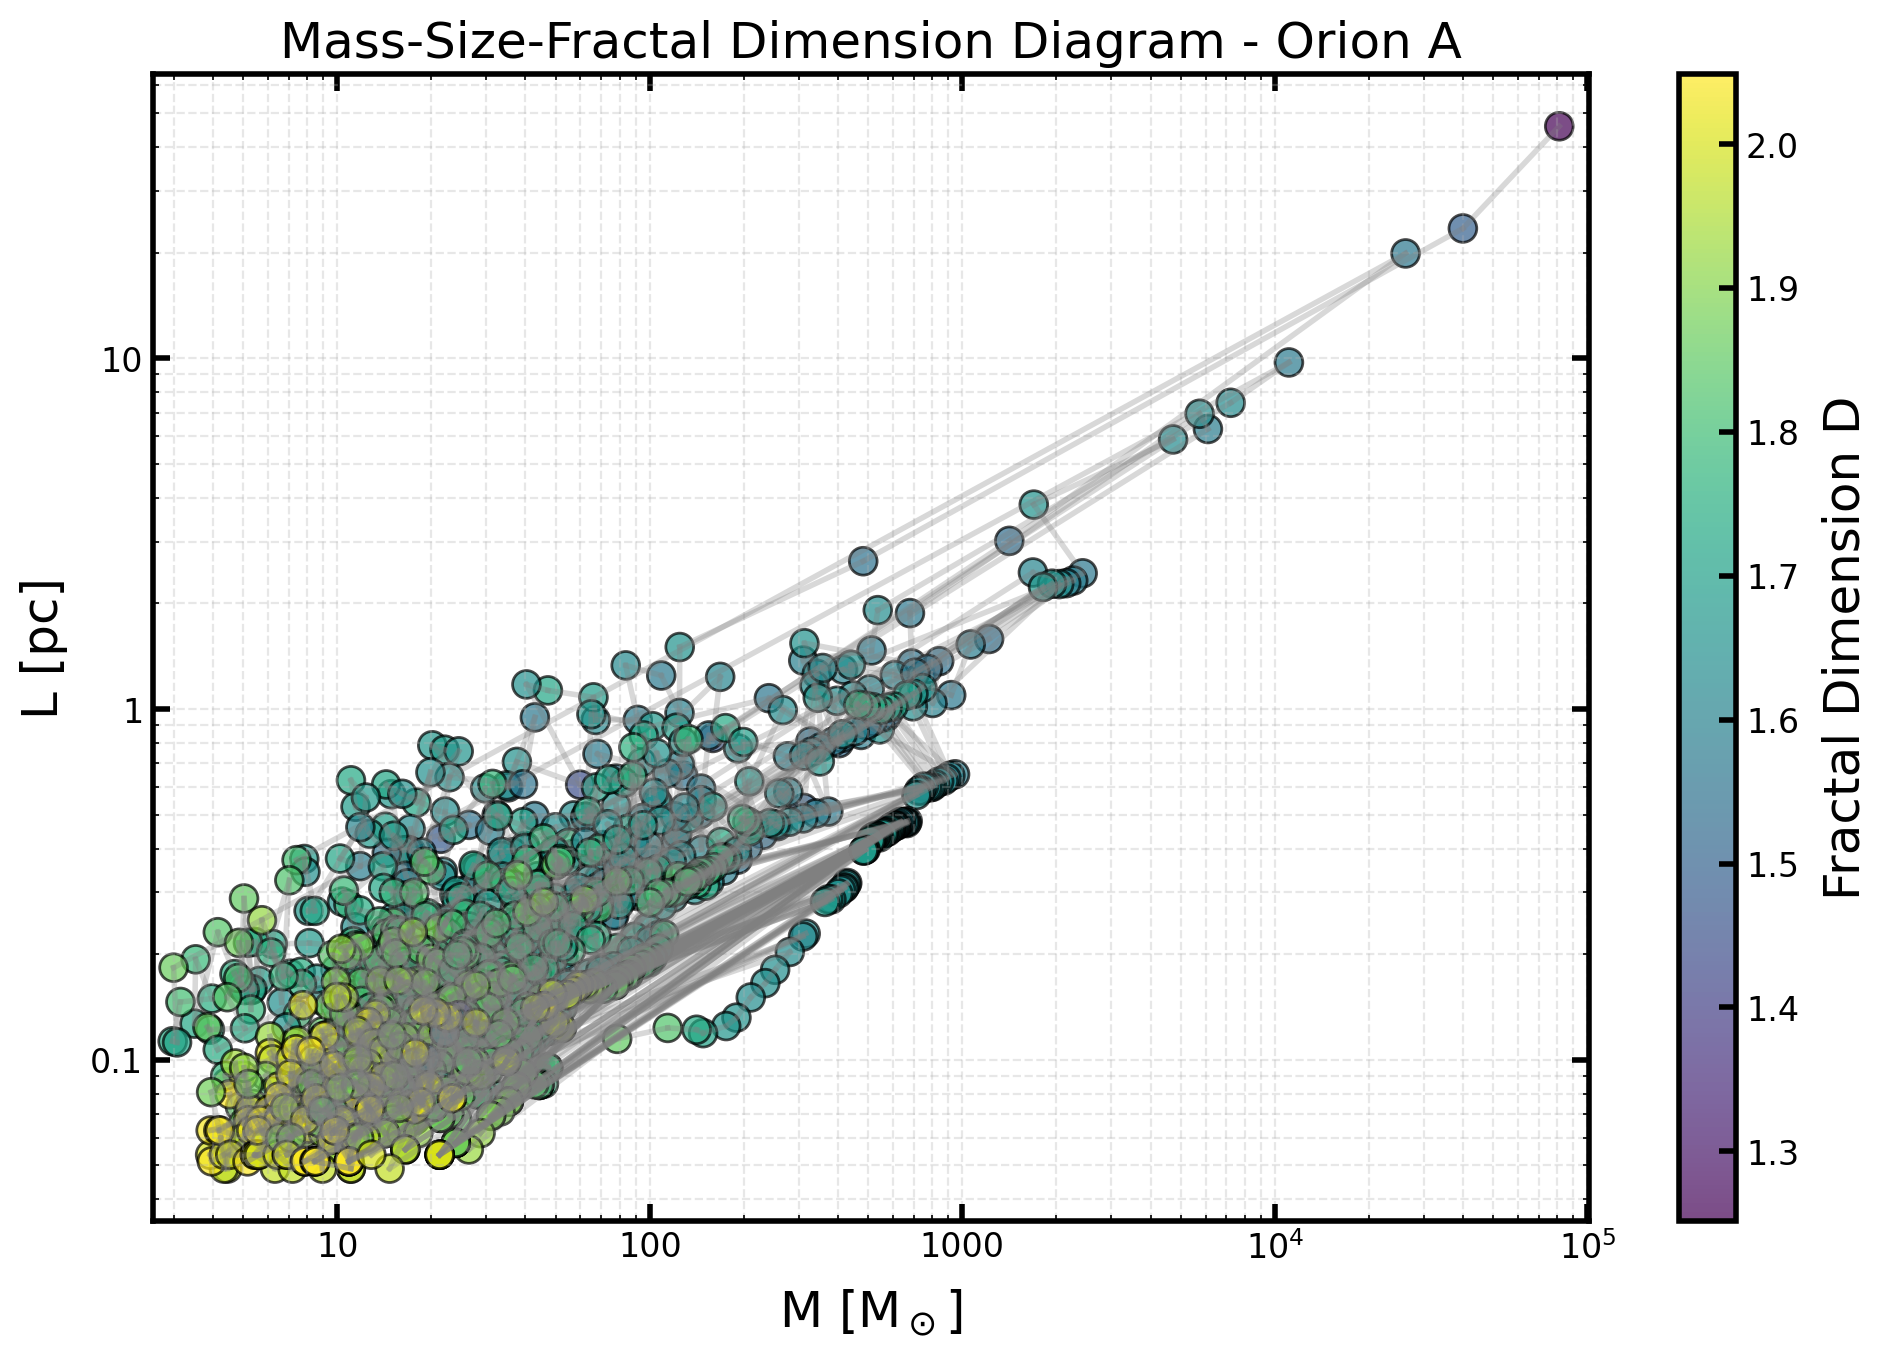
\includegraphics[width=0.5\textwidth]{figures/MSD_Orion_A_with_lines.png}
    \caption{MSD plane for Orion~A with dendrogram connections overplotted. Lines trace parent-child relationships between structures.}
    \label{fig:MSD_orion_A_lines}
\end{figure}

\begin{figure}[h]
    \centering
    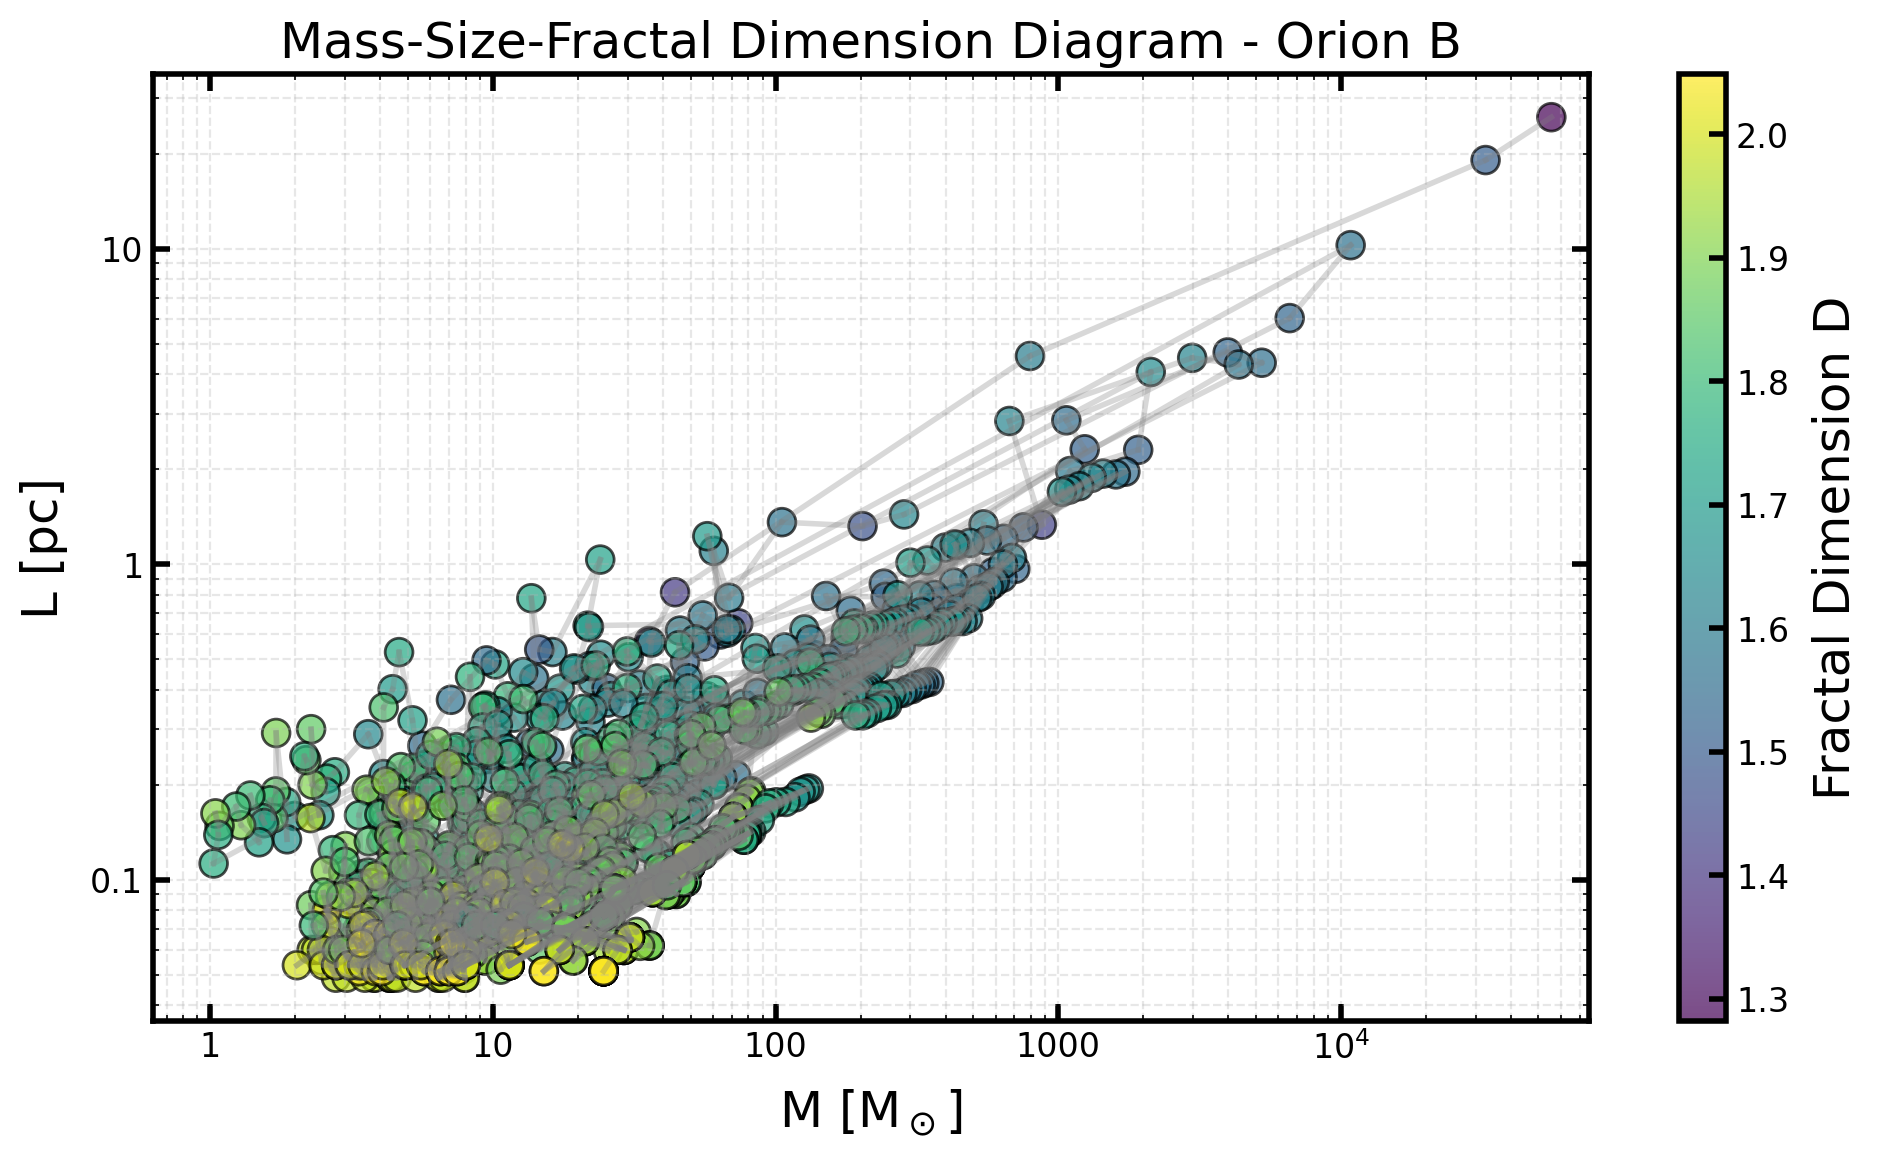
\includegraphics[width=0.5\textwidth]{figures/MSD_Orion_B_with_lines.png}
    \caption{MSD plane for Orion~B with dendrogram connections overplotted.}
    \label{fig:MSD_orion_B_lines}
\end{figure}

\section{YSO Density Maps}

This section of the appendix provides the YSO density maps used in the correlation analysis discussed in the main text.  

\subsection{Class I/flat-spectrum sources}

The following maps show the surface density of early‑stage YSOs (Class~I and flat‑spectrum) for Orion~A and Orion~B.  
These objects are most closely associated with ongoing star formation and are used in the analysis to trace regions of active star‑forming activity.

\begin{figure}[h]
    \centering
    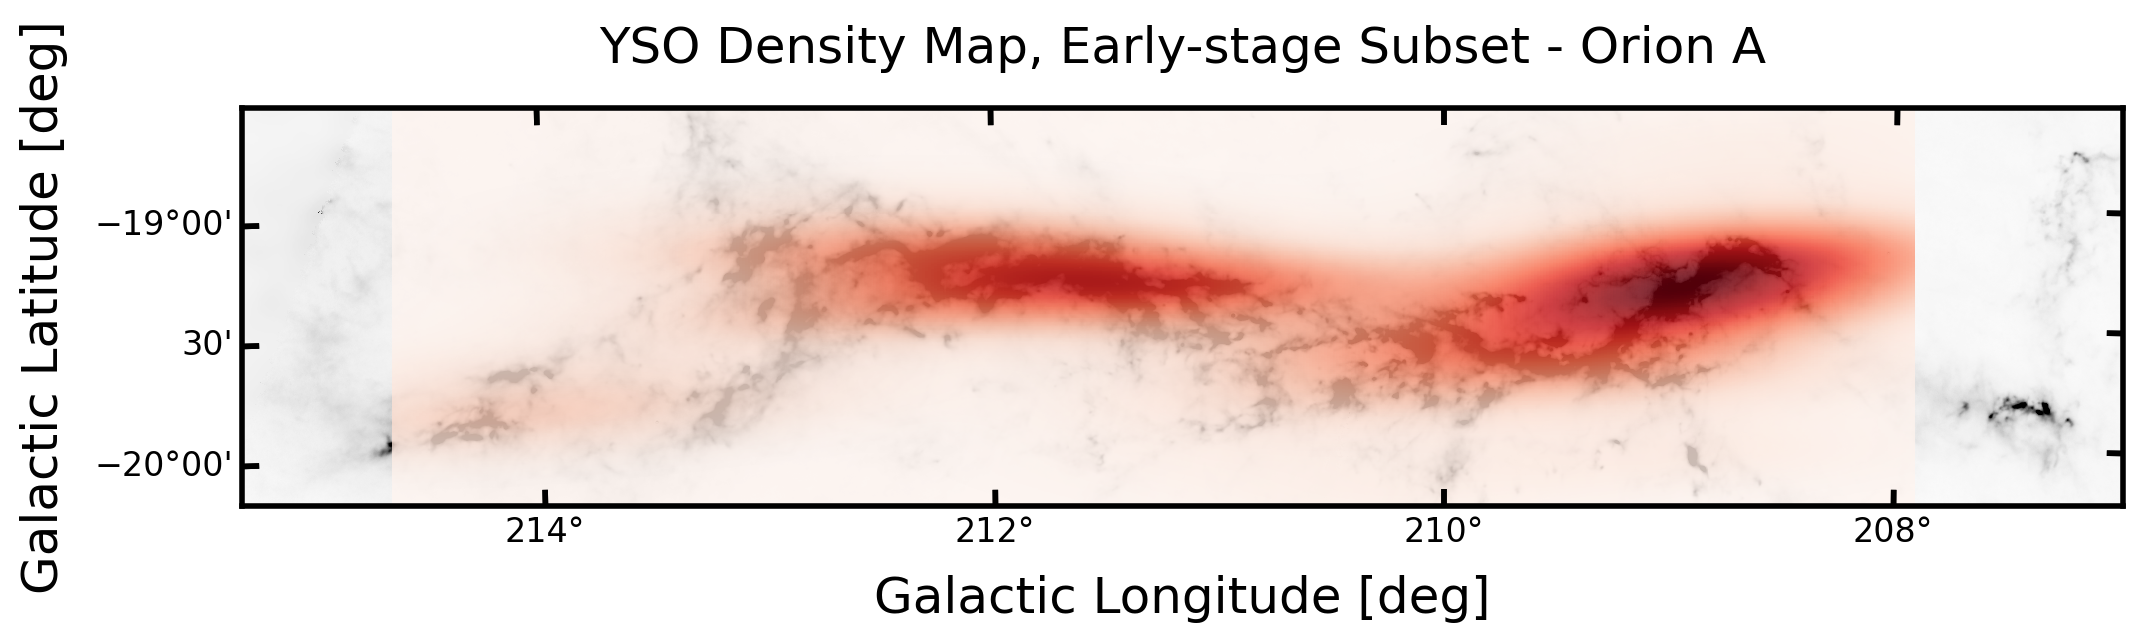
\includegraphics[width=0.75\textwidth]{figures/YSOs_early_stage_density_Orion_A.png}
    \caption{YSO density map for Orion~A, overlaid on the column-density map. The coverage is limited by the extent of the YSO catalog, so some regions are not sampled.}
    \label{fig:YSOs_density_Map_A_early_stages}
\end{figure}

\begin{figure}[h]
    \centering
    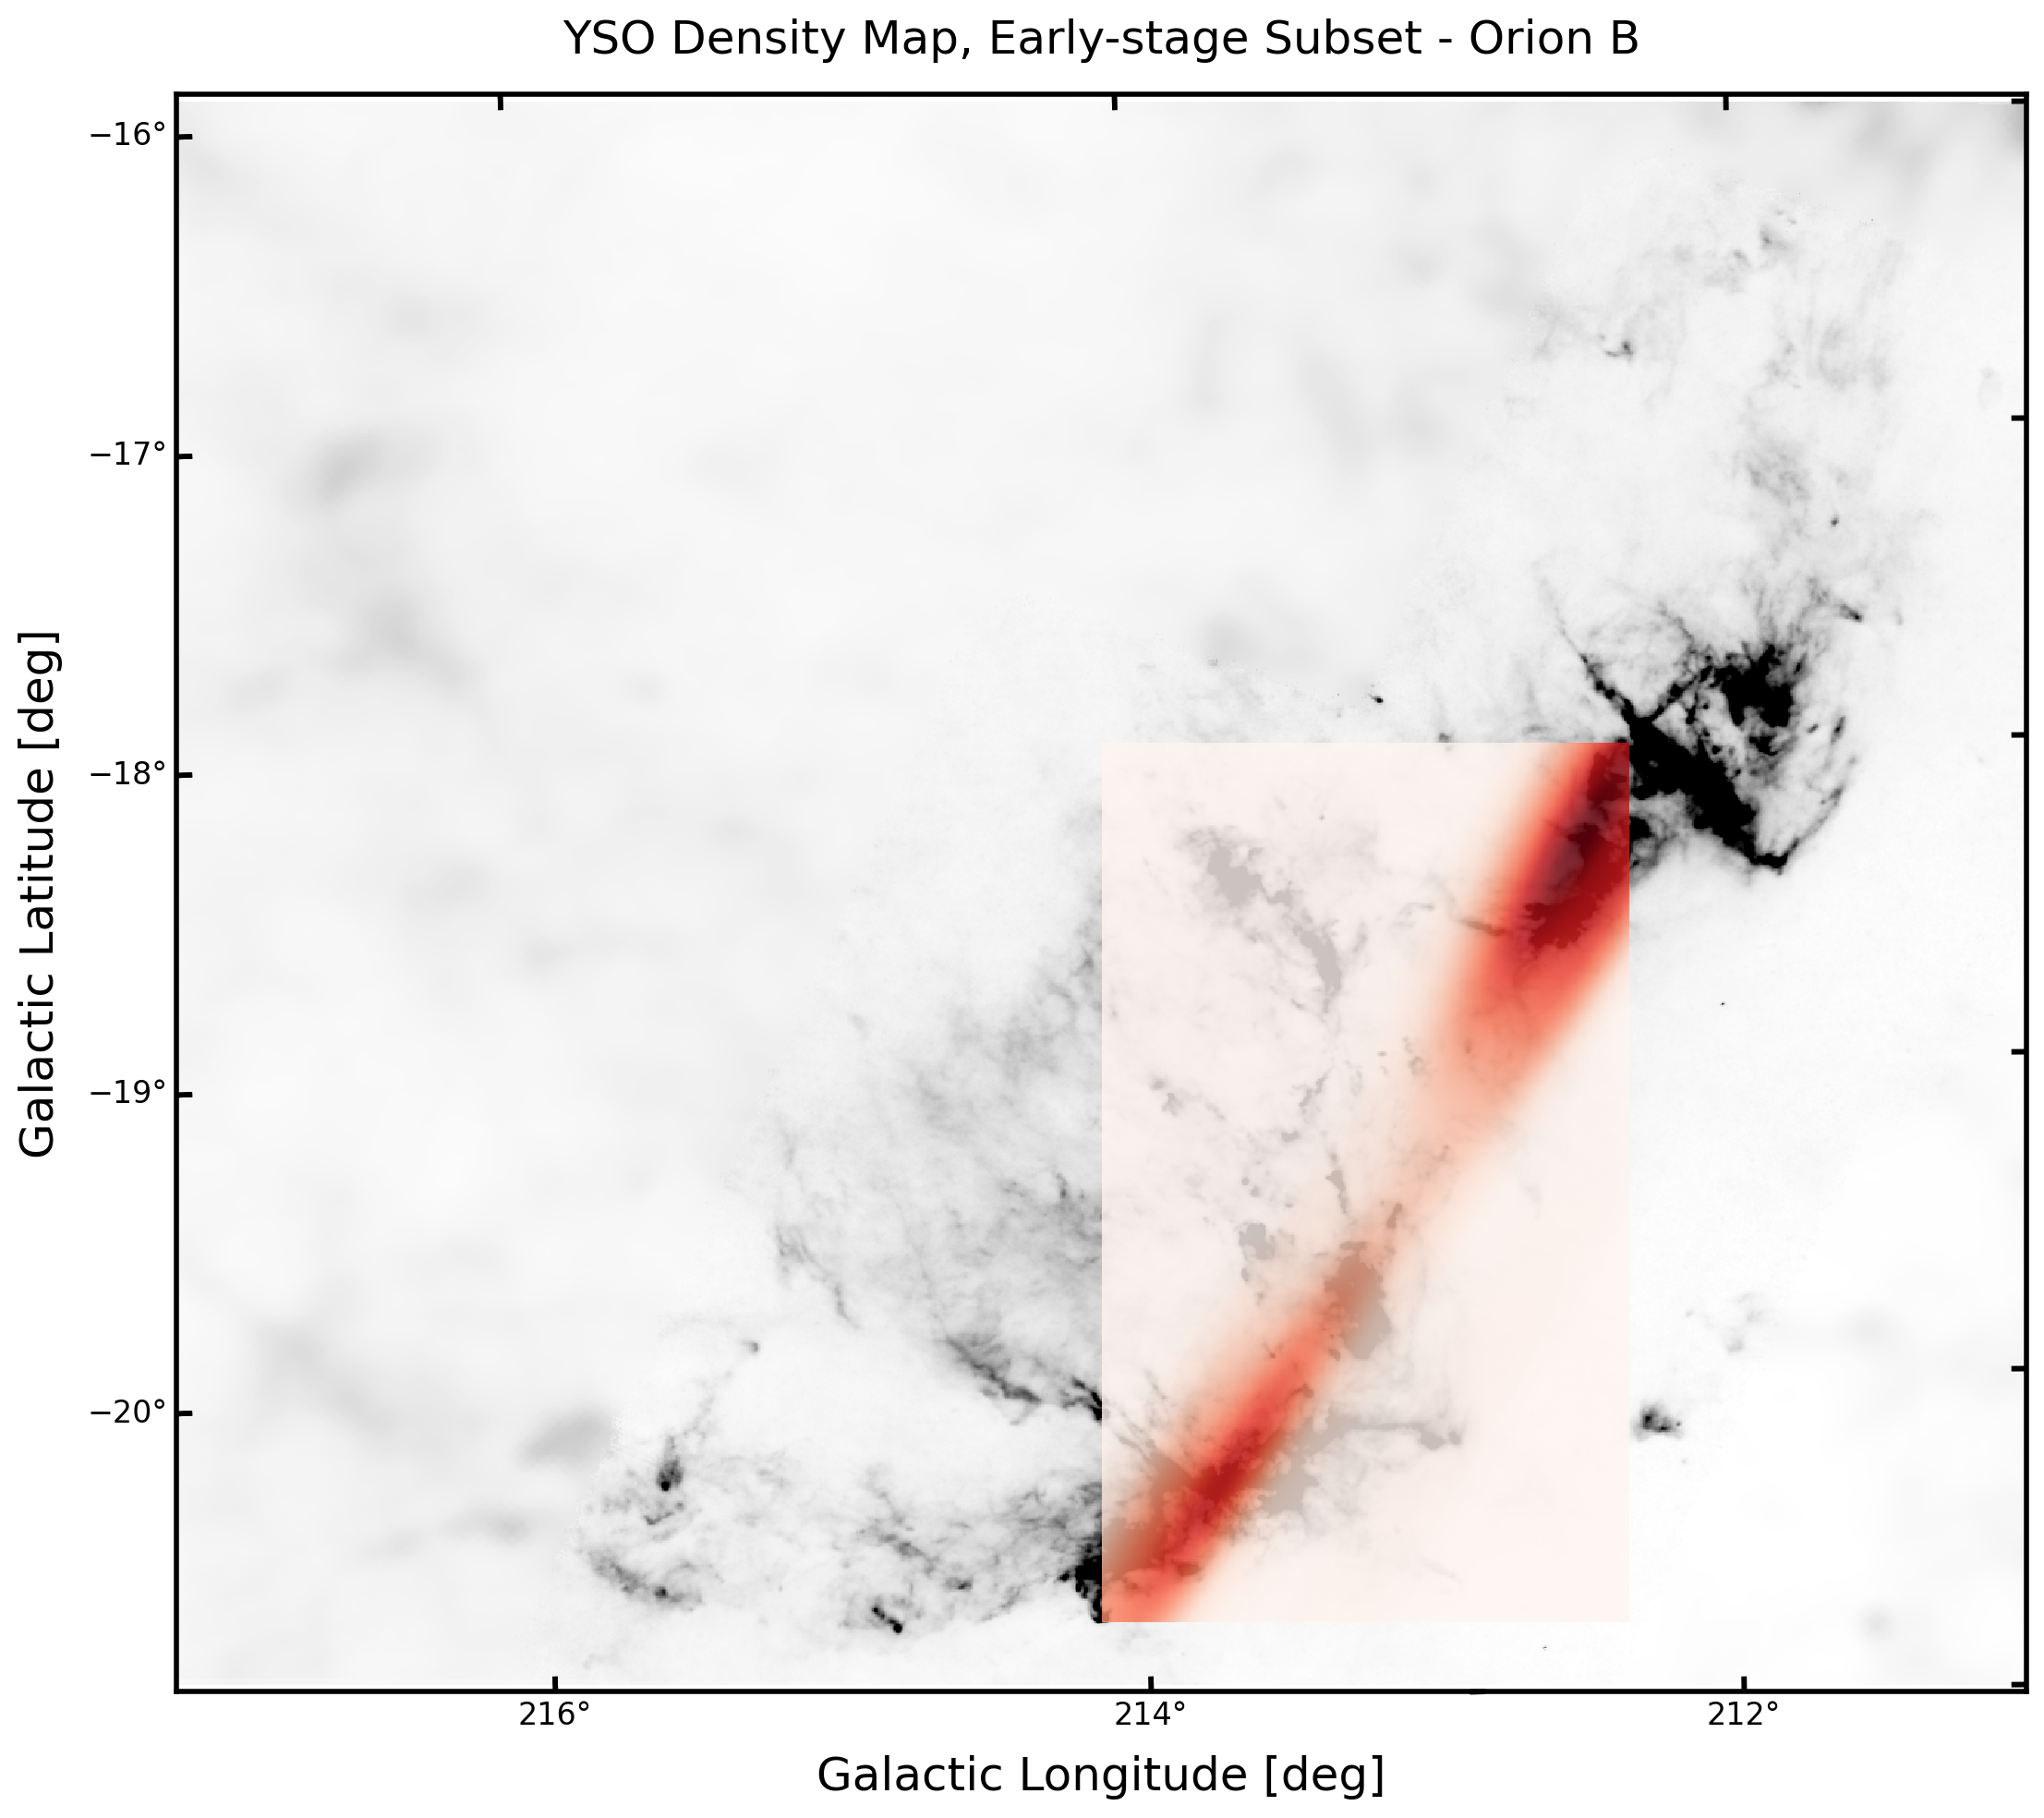
\includegraphics[width=0.5\textwidth]{figures/YSOs_early_stage_density_Orion_B.png}
    \caption{YSO density map for Orion~A, overlaid on the column-density map. The coverage is limited by the extent of the YSO catalog, so some regions are not sampled.}
    \label{fig:YSOs_density_Map_B_early_stages}
\end{figure}

\subsection{Full Sample}

The next set of maps shows the surface density for the full YSO sample, including more evolved Class~II sources.  
These maps provide a broader view of the stellar content but include stars that may have migrated from their birth sites, resulting in a more diffuse distribution.

\begin{figure}[h]
    \centering
    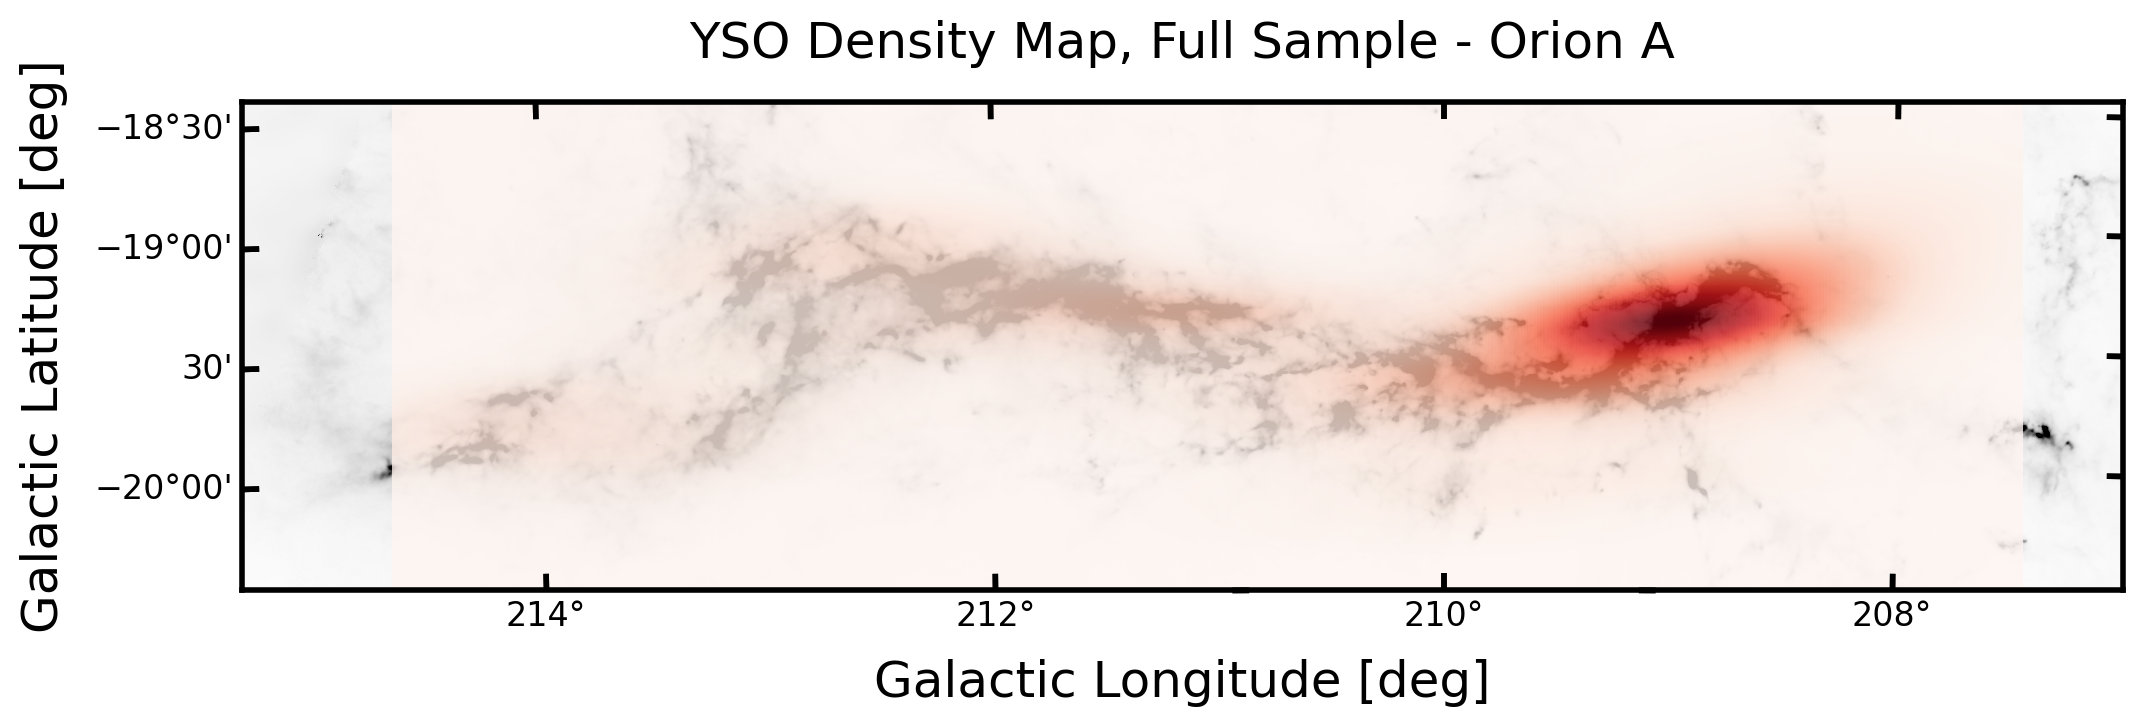
\includegraphics[width=0.75\textwidth]{figures/YSOs_density_Orion_A.png}
    \caption{YSO density map for Orion~A, overlaid on the column-density map. The coverage is limited by the extent of the YSO catalog, so some regions are not sampled.}
    \label{fig:YSOs_density_Map_A}
\end{figure}

\begin{figure}[h]
    \centering
    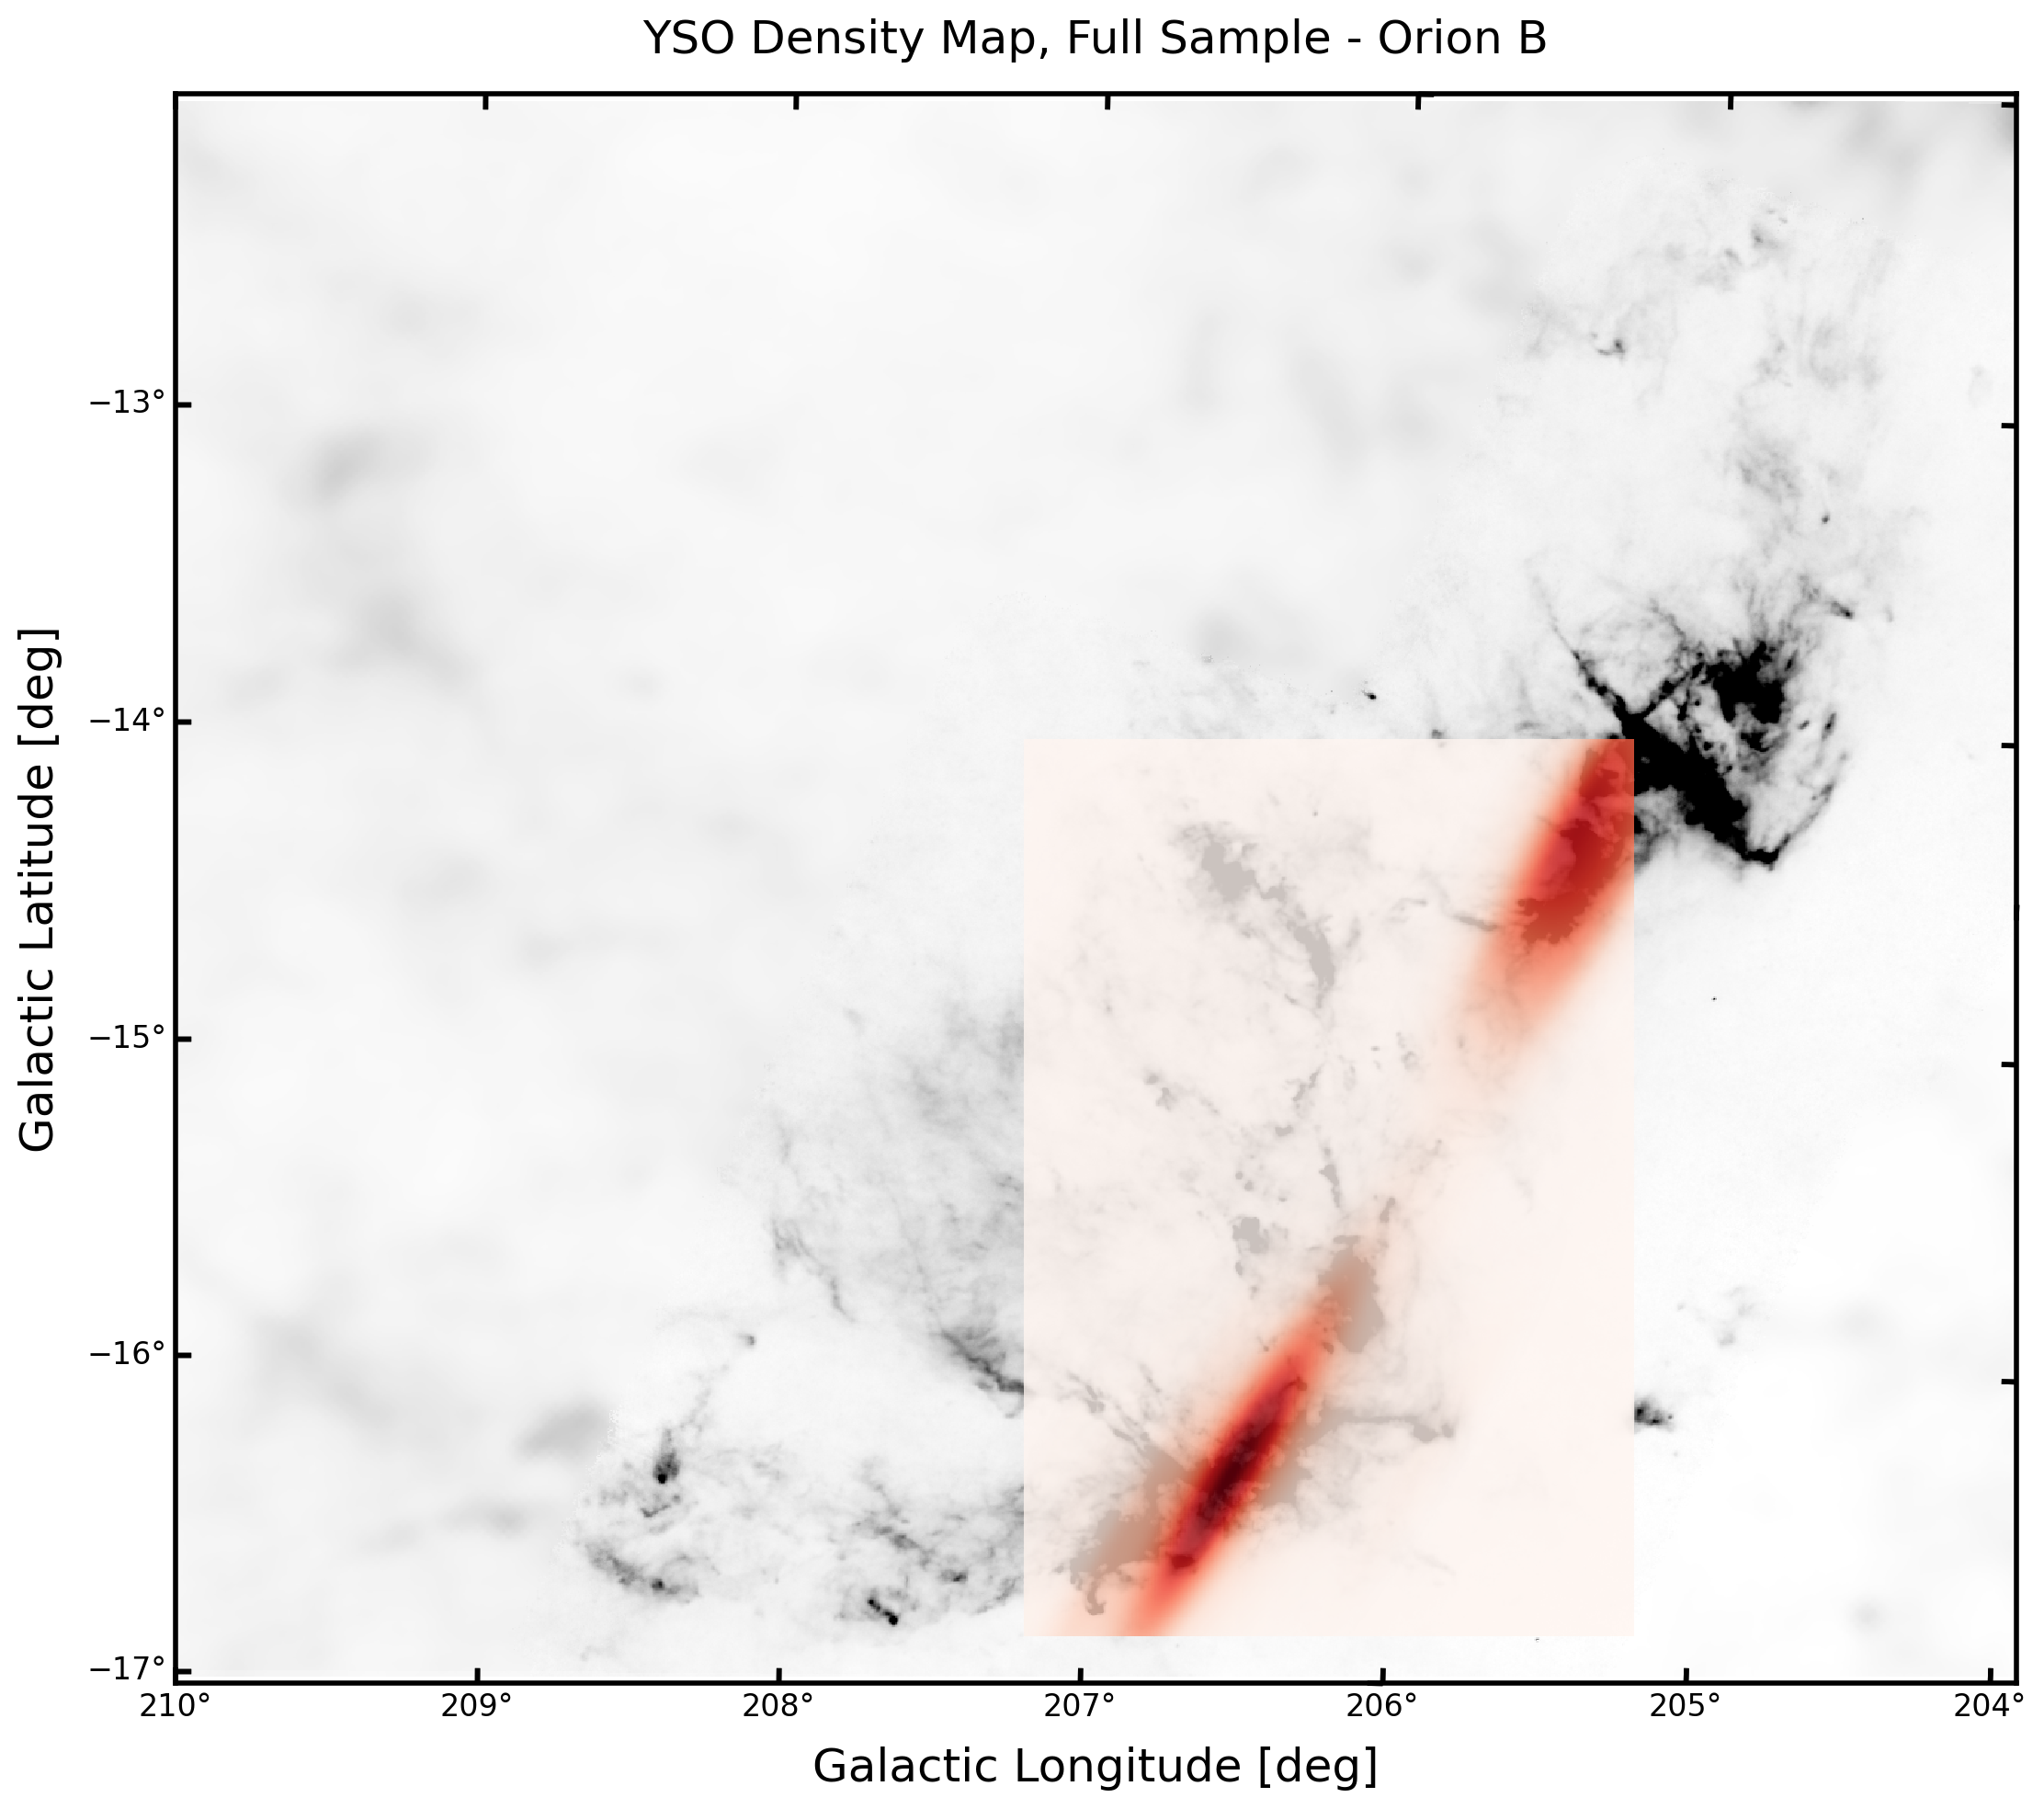
\includegraphics[width=0.5\textwidth]{figures/YSOs_density_Orion_B.png}
    \caption{YSO density map for Orion~A, overlaid on the column-density map. The coverage is limited by the extent of the YSO catalog, so some regions are not sampled.}
    \label{fig:YSOs_density_Map_B}
\end{figure}

\section{Simulations}

This section of the appendix provides more context to the results of the simulations and calculation of the uncertainties.

\subsection{Global Fractal Dimension}
% simulations global fractal dimension: D = 1 for simple shapes, gets higher the more complex it becomes 
% simulations global fractal dimension: GRF (scale free vs with scale) example
% simulations global fractal dimension: resolution effects

\subsection{Local Fractal Dimension}
% simulations local fractal dimension: resolution effects

\subsection{Euler Characteristic}

\subsection{Uncertainties}

\begin{figure}[h]
    \centering
    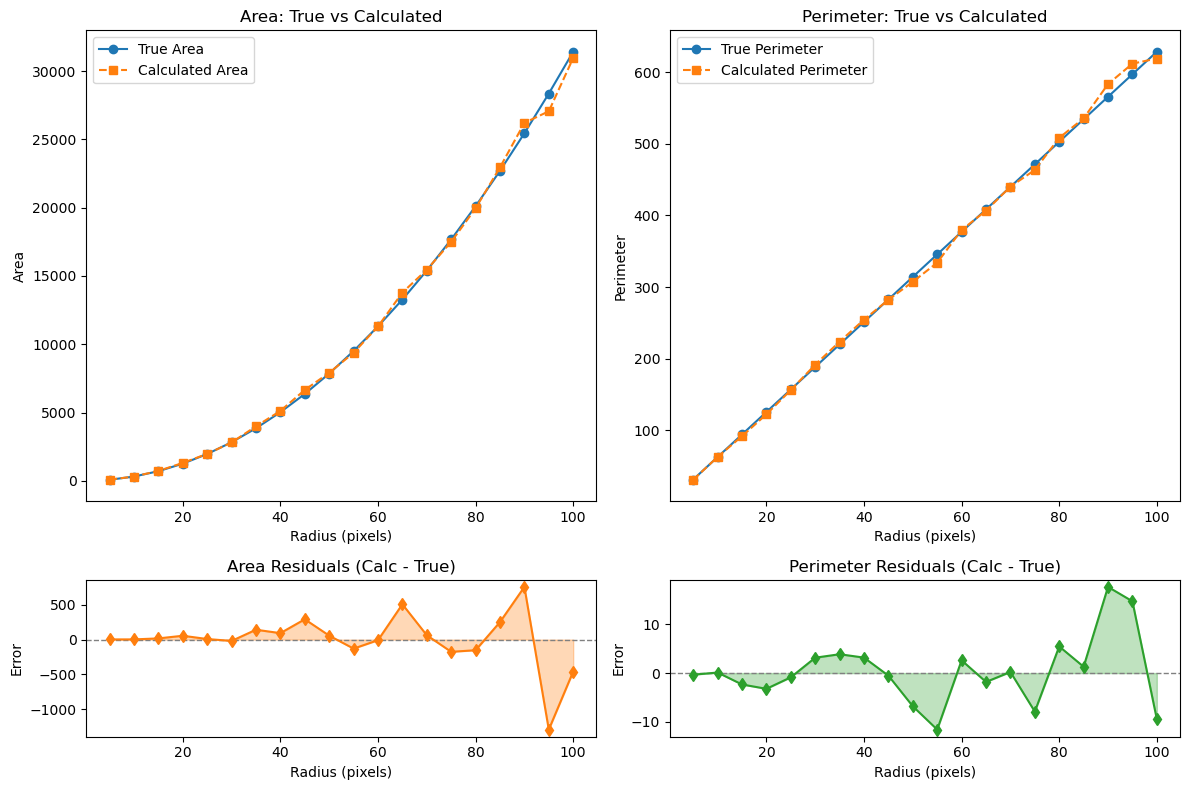
\includegraphics[width=0.75\textwidth]{figures/perimeter_area_uncertainties.png}
    \caption{Example of the uncertainty distributions in the measurements of perimeter and area from simulated structures (arbitrary units).}
    \label{fig:uncertainties}
\end{figure}

	
	
	
\end{document}